%-----------------------------------------------------------------------
%
% File Name: thesis.tex
%
% Author: Swetha Bhagwat
%
% Revision: $Id$
%
%-----------------------------------------------------------------------

% document class and packages
\documentclass[12pt,notitlepage]{report}
\usepackage{bibunits}
\usepackage{suthesis}
\usepackage{graphicx}
\usepackage{color}
\usepackage{amsmath}
\usepackage{amssymb}
\usepackage{amsfonts}
\usepackage[bookmarksnumbered, bookmarksopen, breaklinks, colorlinks, linkcolor=blue, citecolor=magenta]{hyperref}
\usepackage{subfig}
\usepackage{tabularx}
\usepackage{adjustbox}
%\usepackage{caption}
%\usepackage{rotating}
%\usepackage{tensor}

\usepackage{booktabs}

\usepackage{minted}
%%%%%%%%%FROM KERRNESS%%%%%%%%%%%%

\usepackage{graphics}
\usepackage[caption=false]{subfig}
\usepackage{float}
\usepackage{amsmath}
\usepackage{amssymb}
\usepackage[normalem]{ulem} %for \sout
\usepackage[mathscr]{euscript}
\usepackage{acronym}
\usepackage[dvipsnames]{xcolor}
%\usepackage{float}
\floatstyle{boxed}
\usepackage{lipsum}
\usepackage[section]{placeins}
\usepackage{mathtools}
\usepackage{multirow}
\usepackage{graphicx}
\usepackage{xspace}
\usepackage{tikz}
\usepackage{rotating}
\usepackage{microtype}
\usetikzlibrary{shapes,arrows}
\usetikzlibrary{matrix}
\usetikzlibrary{er,positioning}
\DeclareMathAlphabet\mathpazo{OML}{zplm}{m}{it}
%\usepackage[dvipsnames]{xcolor}
%% RCS Id macro \rcsid
\def\thercsid{\relax}
\def\rcsid#1{\def\next##1#1{\def\thercsid{##1}}\next}
\rcsid$Id: QNM.tex,v  Doc No. $
\renewcommand{\today}{\number\day\space\ifcase\month\or
January\or February\or March\or April\or May\or June\or
July\or August\or September\or October\or November\or December\fi
\space\number\year}

\usepackage[colorlinks, pdfborder={0 0 0}, plainpages=false]{hyperref}
\usepackage{graphicx}
\usepackage[caption=false]{subfig}
\captionsetup[subfigure]{labelformat=brace}
\usepackage{xspace}

\usepackage{mathrsfs}






\pdfoutput=1
\DeclareGraphicsExtensions{.pdf,.png}

\hbadness=10000

% new command definitions
\newcommand{\half}{\frac{1}{2}}
\newcommand{\ospsd}{\ensuremath{S_n\left(\left|f_{k}\right|\right)}}

% journal definitions
\newcommand{\apj}{{\it Astrophysical J.}}
\newcommand{\apjl}{{\it Astrophysical J.}}
\newcommand{\aap}{{\it Astron. and Astrophys.}}
\newcommand{\cmp}{{\it Commun. Math. Phys.}}
\newcommand{\grg}{{\it Gen. Rel. Grav.}}
\newcommand{\cqg}{{\it Class. Quant. Grav.}}
\newcommand{\lr}{{\it Living Reviews in Relativity}}
\newcommand{\mnras}{{\it Mon. Not. Roy. Astr. Soc.}}
\newcommand{\pr}{{\it Phys. Rev.}}
\newcommand{\prl}{{\it Phys. Rev. Lett.}}
\newcommand{\prd}{{\it Phys. Rev. D}}
\newcommand{\pra}{{\it Phys. Rev. A}}
\newcommand{\prsl}{{\it Proc. R. Soc. Lond. A}}
\newcommand{\ptrsl}{{\it Phil. Trans. Roy. Soc. London}}
\newcommand{\rmp}{{\it Rev. Mod. Phys.}}

\newcommand{\tcr}{\textcolor{red}}
\newcommand{\tcb}{\textcolor{blue}}
\newcommand{\tcm}{\textcolor{magenta}}
\newcommand{\tcg}{\textcolor{green}}
\newcommand{\tcp}{\textcolor{purple}}




\newcommand{\Msun}{\ensuremath{\mathrm{M}_\odot}}


\begin{document}
\title{Towards probing the strong field gravity using Binary Black-hole ringdowns}
\author{Swetha Bhagwat}
\majorprof{Duncan A. Brown}
\previousdegree{}{B.S-M.S, Indian Institute of Science Education and Research (IISER), Pune}
%\previousdegree{M.S. Syracuse University, Syracuse, NY, 2013}{}
\submitdate{June 2018}
\degree{Doctor of Philosophy}
\program{Physics}
\copyrightyear{2018}
\majordept{Physics}
\atitlep
\clearpage
\havededicationtrue
\dedication{dedication}
\haveminorfalse
\copyrighttrue
\doctoratetrue
\figurespagetrue
\tablespagetrue
\electronicsubmitfalse

\Abstract{
In this thesis, we explore the tools necessary to probe the strong-field gravity using a binary black hole ringdown. When two black holes merge, they form a single distorted black hole that then radiates gravitational waves and settles into a final stable Kerr state. The signal produced during this process is called the ringdown and can be modelled as perturbations on the space-time of the final Kerr black hole. Ringdowns contain information about the strong field dynamics close to the black holes and thus, can be used to test our understanding of gravity. There are three specific questions that we explore in this thesis: First, at what point after the merger of two black holes can one use a perturbative description to model the space-time? This tells where in the gravitational wave signal of a binary black hole merger can one start a ringdown-based test. Second, how likely are we to realistically find a signal that allows us to perform a ringdown-based test given the current and future gravitational wave observatories. And finally,  how should the data analysis be carried out in order to extract information from the ringdown of an observed GW signal? 
}

%\Acknowledgments{
%% $Id$

As a member of the LIGO Scientific Collaboration, I have been fortunate to
have benefited through advice from and discussions with many people. It would
not be possible to thank everyone who I have worked with over the past five
years without making the acknowlegements longest chapter in this dissertation,
so I shall only attempt to thank those who I have interacted with the most and
hope that the others forgive me.

First and foremost, I would like to thank Patrick Brady. I am fortunate to
have an advsior whose as big a drunk as I am.

I would also like to thank Jolien Creighton for his help and enthusiasm over
the past five years. It has been fun working with Jolien and I have learnt a
great deal from him through his patient explanations.

I am greatful to Bruce Allen for suggesting the search for binary inspiral as
a research topic and his assitance with the scientific and computational
obstacles along the way. Thanks also to Gabriela Gonz\'{a}lez for patiently
anserwing my many stupid questions about the LIGO interferometers helping me
understand the data that I have been analyzing.

I would like to thank the members of my committee: Daniel Agterberg, John
Friedman and Leonard Parker for their careful reading of this dissertation and
helpful suggestions for its improvement.

I also would like to thank Warren Anderson, Teviet Creighton, Stephen
Fairhurst, Scott Koranda, Eirini Messaritaki, Ben Owen, Xavier Siemens and
Alan Wiseman for help, advice and pints of beer. I am also indebted to Axel's
for many useful discussions.

Thanks to Steve Nelson, Wyatt Osato and Quiana Robinson for their help in the
preparation of this this and, of course, to Sue Arthur for making everything
run smoothly.

I could not have come this far without the constant love and support of my
parents, to whom this thesis is dedicated. Finally, I would like to thank
Emily Dobbins for all the love and understanding over the past two years.
}

\beforepreface

%\prefacesection{Preface}
%Need to write the Preface

\afterpreface

%\Chapter{Introduction}
%\label{ch:introduction}
%In 1915, Albert Einstein published his theory of general relativity, a 
geometric theory of gravitation that sought to expand upon Newtonian 
mechanics and provide a complete description of gravity and its 
relationship with space and time. Einstein theorized that space 
and time were deeply related and existed together as a manifold 
called spacetime. Matter with energy and momentum 
existing in this manifold would create 
curvature in spacetime. Gravitational forces were the result of 
matter following geodesic curves in spacetime. This concept can 
be summarized in the Einstein field equation, which is presented 
as,
\begin{equation}
G_{\mu\nu} = 8\pi T_{\mu\nu}
\label{eq:EFE}
\end{equation}
where $G_{\mu\nu}$ is the Einstein tensor, which describes the 
curvature of spacetime, $T_{\mu\nu}$ is the 
stres-energy tensor, which describes the energy and momentum in 
spacetime, and  $G=c=1$. The Einstein tensor is defined as,
\begin{equation}
G_{\mu\nu} = R_{\mu\nu} - \frac{1}{2}Rg_{\mu\nu}
\end{equation}
where $R_{\mu\nu}$ is the Ricci curvature tensor and $g_{\mu\nu}$ is 
the metric tensor for the manifold.

An interesting result that arises from this formalism is the 
existence of gravitational waves, which are perturbations in 
spacetime caused by certain types of time-varying mass distributions. 
To describe gravitational waves, we consider 
a Minkowski metric with a small perturbation. The Minkowski metric 
is a flat spacetime metric defined as
\begin{equation}
\eta_{\mu\nu} = 
  \begin{pmatrix}
   -1 & 0 & 0 & 0 \\
    0 & 1 & 0 & 0 \\
    0 & 0 & 1 & 0 \\
    0 & 0 & 0 & 1
  \end{pmatrix}
\end{equation}
where $\mu = 0$ corresponds to the time coordinate and $\mu = {1,2,3}$ 
correspond to the spatial coordinates. In examples, we will use the coordinate 
convention $(x^0,x^1,x^2,x^3) = (ct,x,y,z)$. 
The full spacetime metric, $g_{\mu\nu}$, is then constructed as a 
linear perturbation on the Minkowski metric,
\begin{equation}
g_{\mu\nu} = \eta_{\mu\nu} + h_{\mu\nu}
\end{equation}
where $h_{\mu\nu}$ is the metric perturbation and $|h_{\mu\nu}| \ll 1$.
From here, we follow the convention of Saulson \cite{Saulson:1994} to arrive at the general 
form of a gravitational wave.
At this point it is very useful to move into the transverse traceless 
gauge where coordinates on the manifold are defined by the geodesic 
motion of freely-falling test masses. In this gauge, the weak field 
vacuum solution of the Einstein field equation becomes a wave equation: 
\begin{equation}
\square h_{\mu\nu} = 0.
\end{equation}
The solutions to this differential equation will be plane waves of 
the form
\begin{equation}
h_{\mu\nu} = C_{\mu\nu}e^{i(2\pi ft - \vec{k}\cdot\vec{x})}
\end{equation}
where $C_{\mu\nu}$ is the wave amplitude, $f$ is the frequency, 
and $\vec{k}$ is the wave vector which indicates the direction of 
propagation \cite{Carroll}.

For example, consider the case of a gravitational 
wave propogating along the $\hat{z}$-axis.
When the conditions of the transverse traceless gauge are applied, 
the resulting form of $h_{\mu\nu}$ is 
\begin{equation}
h_{\mu\nu} = 
  \begin{pmatrix}
    0 & 0 & 0 & 0 \\
    0 & h_+ & h_x & 0 \\
    0 & h_x & -h_+ & 0 \\
    0 & 0 & 0 & 0
  \end{pmatrix}
\end{equation}
where the diagonal and off-diagonal terms represent two polarizations 
of the resulting gravitational wave, called "h-plus" and "h-cross" 
respectively.
We can see the effects of this perturbation by observing the  
spacetime interval on the manifold. The spacetime interval is defined as 
\begin{equation}
ds^2 = dx^\mu g_{\mu\nu}dx^\nu.
\end{equation}
Substituting in our perturbed metric for $g_{\mu\nu}$, we find that 
the spacetime interval can be broken up into a standard Minkowski line 
element and a perturbation due to $h_{\mu\nu}$.
\begin{equation}
ds^2 = dx^\mu (\eta_{\mu\nu} + h_{\mu\nu})dx^\nu \\
\end{equation}
\begin{equation}
ds^2 = dx^\mu \eta_{\mu\nu} dx^\nu + dx^\mu h_{\mu\nu}dx^\nu
\label{eq:spacetime}
\end{equation}

As an example, we present the case of a plus-polarized gravitational wave 
propagating in the $\hat{z}$ direction and observe the effect of the perturbation 
on the spacetime interval. The perturbation will have the form 
\begin{equation}
h_{\mu\nu} = 
  \begin{pmatrix}
    0 & 0 & 0 & 0 \\
    0 & h_+ & 0 & 0 \\
    0 & 0 & -h_+ & 0 \\
    0 & 0 & 0 & 0
  \end{pmatrix}
\end{equation}
Using the coordinate convention of $(ct,x,y,z)$, the unperturbed
spacetime interval is given as: 
\begin{equation}
ds^2 = -c^2 dt^2 + dx^2 + dy^2 + dz^2.
\end{equation}
Since the perturbation is spatially transverse to the direction of 
propagation, the ct- and z-coordinates will not be modulated by the 
gravitational wave. The x- and y-coordinates will be modulated  
according to equation \ref{eq:spacetime}. The resulting spacetime 
interval is
\begin{equation}
ds^2 = -c^2 dt^2 + (1 + h_+)dx^2 + (1 - h_+)dy^2 + dz^2.
\end{equation}
This shows that a gravitational wave propogating along the $\hat{z}$-axis 
will differentially stretch and squeeze spacetime in the transverse 
axes. The exact form of $h_+$ will depend on the source of the 
gravitational waves. A visualization of this stretching and squeezing 
is shown in Figure \ref{fig:polarizations}\cite{Polarization}. The cross polarization  
stretches and squeezes at a 45 degree angle relative to the plus 
polarization.

\begin{figure}[ht!]
\includegraphics[width=\textwidth]{figures/introduction/polarisations2}
\caption[Plus and cross polarizations]{Plus and cross polarizations %
         of a gravitational wave.}
\label{fig:polarizations}
\end{figure}

The Advanced LIGO interferometers are designed to be sensitive 
to this differential stretching and squeezing by constructing orthogonal 
optical cavities. A gravitational wave passing through an aLIGO interferometer 
will differentially 
modulate the lengths of the optical cavities, creating an interference 
pattern at the output of the instrument that can be searched for 
gravitational wave signals. The layout and gravitational wave readout scheme 
of the interferometers is discussed below.

\section{The Advanced LIGO Interferometers}\label{sec:aligo}

The Advanced LIGO (aLIGO) interferometers are a pair of dual-recycled Michelson interferometers 
that employ 4km long Fabry-Perot cavities in their arms to increase the interaction time with a 
gravitational wave signal. 
Figure \ref{fig:aligo} shows a simplified layout of an aLIGO interferometer. 

\begin{figure}[ht!]
\includegraphics[width=\textwidth]{figures/introduction/ALIGO_layout}
\caption[Layout of Advanced LIGO]{Layout of Advanced LIGO}
\label{fig:aligo}
\end{figure}

At the input to an aLIGO interferometer is a solid-state Nd:YAG laser that provides laser light 
at a wavelength of 1064 nm. Not included in Figure \ref{fig:aligo} are frequency and 
intensity stabilization control loops designed to provide as stable a laser source as 
possible for the experiment. This stabilized laser is called the pre-stabilized laser 
(PSL). The laser light is passed through a series of 
electro-optic modulators (EOM) where radio-frequency (RF) sidebands are generated 
and imparted onto the light. These RF sidebands are used to control auxiliary optical 
degrees of freedom in the interferometer. The beam is then passed through the 
input mode cleaner (IMC), which rejects higher order spatial modes of the beam 
and transmits a circular TEM00 mode to be used in the instrument.

Once the beam has been stabilized in frequency and intensity and the higher order 
optical modes have been stripped away, it is transmitted through the power 
recycling mirror and enters the vertex of the interferometer. In the vertex, 
the beam is split 50/50 by the beamsplitter. Half of the light is directed toward  
the input test mass (ITM) of the X-arm and half of the light is directed  
toward the ITM of the Y-arm. As mentioned previously, the aLIGO arms are not 
single bounce cavities; they are comprised of Fabry-Perot cavities that allow the 
light to circulate in the arm cavities multiple times. The light is stored in 
the arm cavities for $\sim$1ms, trapped between the highly reflective surfaces 
of the ITM and the end test mass (ETM), before it is transmitted back through 
the ITM and into the vertex.

When a gravitational wave passes through an aLIGO inteferometer, the distance
between the ITM and ETM of each arm is modulated, causing the light to have a
longer or shorter travel time as it traverses the arm. Since gravitational
waves expand space in one direction while the orthogonal direction contracts,     
the X- and Y-arms will experience differential changes in length. When light
from the arms is recombined at the beamsplitter, there will be a difference
in phase between the two beams as they have traveled different paths. The 
resulting light from this recombination of phase shifted beams is called the 
antisymmetric part of the output. The part of the beam that is recombined 
in phase is called the symmetric part of the output.

The beams returning from each arm are recombined at the beamsplitter. The 
symmetric part of the beam 
will be sent back toward the power recycling mirror. The power recycling mirror 
forms a resonant cavity with the ITMs, allowing for light at the symmetric 
port of the beamsplitter to be added coherently to incoming light from the PSL and 
increasing the effective power in the vertex. This increase in effective power 
is known as the power recycling gain. 

The antisymmetric part of the beam is sent toward the signal recycling mirror. 
The signal recycling cavity is used to tune the frequency response of the 
interferometer by adjusting the effective finesse of the coupled cavity 
formed by the signal recycling cavity and the arm cavities. 
If the light returning from the arms has accumulated some differential amount of 
phase as it traveled 
along the arms, perhaps from a gravitational wave modulating the length of each 
arm differentially, it will be transmitted through the signal recycling cavity 
and into the output mode cleaner (OMC). The OMC behaves similarly to the IMC, 
stripping away higher order optical modes and isolating the TEM00 mode of the 
beam. The transmitted, mode cleaned signal is then read out using a homodyne 
detection scheme on a DC photodiode. 

\subsection{DC Readout}

When a gravitational wave modulates the length of an arm cavity, the light 
traveling in that arm experiences a phase modulation. This phase modulation 
can be visualized by picturing the beam in frequency space. In figure 
\ref{fig:omc-freq}, the carrier beam frequency is designated as $f_0$. 
The phase modulation due to 
a gravitational wave signal introduces a frequency sideband at the 
gravitational wave frequency, which is in the 30-2000 Hz range. 
The 
RF sidebands used for auxiliary optical cavity control are offset from the 
carrier frequency by 9, 24, and 45 MHz. 
The RF sidebands, which in a 
homodyne detection scheme would only contribute shot noise to the output signal, 
are rejected by the OMC. The gravitational wave sidebands, however, are at a 
low enough frequency offset that they are within the cavity pole of the OMC 
and are allowed to transmit through the cavity.

Since the OMC DC photodiode measures power, it measures the square of the 
incident optical field and witnesses beat frequencies between different 
components of the light. If the RF sidebands have been filtered out by 
the OMC, the only remaining beat note will be that of the carrier beam ($f_0$) 
beating against the gravitational wave sideband ($f_0 + f_{GW}$). This beat note will 
appear as the difference in frequency between the two optical fields, 
leaving behind a signal in the 30-2000 Hz range ($f_{GW}$) and providing a 
natural demodulation inherent to the measurement process. 
The process of recovering the gravitational wave sideband using the 
carrier field as a reference is known as homodyne detection. 

\begin{figure}[ht!]
\includegraphics[width=\textwidth]{figures/introduction/omc-freq}
\caption[Sidebands and OMC cavity pole]{Frequency domain visualization of beam %
         at OMC. Grey dotted lines indicate the cavity pole. The gravitational %
         wave sidebands are within the cavity pole and are transmitted through %
         the OMC. The RF sidebands are in the MHz range and are rejected by the %
         OMC.}
\end{figure}\label{fig:omc-freq}

\section{Sources of Gravitational Waves}
Include that box with modeled, unmodeled, transient, and continuous.

CBCs are the bread and butter, expect BNS, NSBH, and BBH sources
Continuous waves from pulsars
Bursts from supernovae
Stochastic background


\section{Searching for Compact Binary Coalescences}

Steal this from O1 CBC DQ paper


\section{The Advanced Detector Network}

The Advanced Laser Interferometer Gravitational-Wave Observatory (aLIGO) is 
part of a worldwide effort to detect gravitational waves from astrophysical 
sources. The two aLIGO interferometers, one in Hanford, WA and one in 
Livingston, LA, are part of a growing network of ground-based interferometric 
gravitational wave detectors. Each aLIGO interferometer has 4km long arms 
arranged in an L-shaped configuration. A gravitational wave passing through 
an aLIGO interferometer will cause the arms to expand and contract, 
creating an interferometric signal at the output of the instrument. 
Section \ref{sec:aligo} contains a more detailed description of the aLIGO 
interferometers. 

There are a number of other interferometric gravitational wave detectors 
being built and commissioned for future use in collaboration with aLIGO.
The Advanced VIRGO detector is being built and commissioned in Cascina, Italy. 
When it is fully commissioned, VIRGO will be joining LIGO in observing runs. 
The VIRGO interferometer has 3km arms, which should provide enough 
sensitivity to allow for triangulation of astrophysical sources.

The GEO600 detector, located in Hanover, Germany is an interferometer built in 
collaboration between Germany and the United Kingdom. 
GEO600 is an extremely valuable test bed for interferometric technologies,
including quantum optics and homodyne detection. However, with 600m arms, GEO600 
is unlikely to be sensitive enough to witness expected astrophysical sources.

The KAGRA detector, located underground in the Kamioka mine in Japan, 
is in its commissioning phase. KAGRA has 3 km long arms and, 
unlike other gravitational wave interferometers, employs cryogenics to 
reduce thermal noise in its optics. When complete, KAGRA should be 
sensitive enough to contribute to the worldwide detector network.

Include that cool picture of the advanced detector network.



\Chapter{Introduction}
\label{ch:Introduction}
%Why test Gr

Many of the challenges of 21st-century physics involve our understanding of gravity. Open research problems include: the quantization of gravity \cite{QG1,QG2,QG3,QG4}, the black hole (BH) information paradox \cite{BHIP1,BHIP2,BHIP3,BHIP0,BHIP4}, building a unified theory for the fundamental forces \cite{GUT}, the fine-tuning problem in cosmology \cite{CosmoConstant1,CosmoConstant2} and understanding the nature of the dark energy \cite{DarkEnergy}. The general theory of relativity (GR) which describes the classical behaviour of gravitation \cite{OnGR}, has an elegant theoretical structure and has been tested experimentally in various regimes\cite{ReviewAlternativeTheories1}. Our understanding of gravity seems to conflict with the framework of quantum mechanics \cite{GRvsQM3,GRvsQM1,GRvsQM2} and developing a quantum theory of gravity is an open problem.  Also, the fine-tuning problem in cosmology suggests that our understanding of gravity is incomplete at the large scales. Given the incomplete nature of GR, alternative descriptions of gravitation are being developed that aim to resolve one or more of these inconsistencies \cite{ReviewAlternativeTheories1,ReviewAlternativeTheories2,ModifiedGravity1,ModifiedGravity2}. Experimental and observational tests of GR and other alternative theories of gravity are needed to understand the nature of gravity \cite{kipTGR1,kipTGR2,kipTGR3,TGRwithLISA}.

%Many of the challenges of 21st-century physics involve our understanding of gravity. For example, the quantization of gravity \cite{QG1,QG2,QG3,QG4}, the black hole information paradox \cite{BHIP1,BHIP2,BHIP3,BHIP0,BHIP4}, building a unified theory for the fundamental forces \cite{GUT}, the fine-tuning problem in cosmology \cite{CosmoConstant1,CosmoConstant2} and the understanding of the nature of the dark energy \cite{DarkEnergy} . The general theory of relativity (GR) describes the classical behaviour of gravitation \cite{OnGR}. Not only does GR have an elegant theoretical structure, but has also been validated by experiments in various regimes\cite{ReviewAlternativeTheories1}. However, developing a theory of gravity on a quantum scale is still an avid problem. While our understanding of gravity seems conflicting with the framework of quantum mechanics \cite{GRvsQM3,GRvsQM1,GRvsQM2}, at large scales, we encounter the problem of fine-tuning of the cosmological constant. Given the incomplete nature of GR, alternative descriptions of gravitation are being developed that aim to resolve one or more of these inconsistencies \cite{ReviewAlternativeTheories1,ReviewAlternativeTheories2,ModifiedGravity1,ModifiedGravity2}. Given the circumstance, experimental and observational lead seems imperative to further our understanding of Gravity. Experimental and observational tests of GR and other alternative theories of gravity are needed to truly understand the nature of gravity \cite{kipTGR1,kipTGR2,kipTGR3,TGRwithLISA}. 

%Intro to GW as a tool for TGR
Metric theories of gravity, predict propagating disturbances in space-time curvature known as the gravitational waves (GW) \cite{kipGWGR}. The details of these GWs depend on the exact underlying theory of gravity \cite{ReviewAlternativeTheories1}.  A measurement of GW can help eliminate or constrain families of alternative theories of gravity and test GR. Observing GW signals from collision of two BHs \cite{CBCGW1, CBCGW2} can help us understand the nature of gravity.

%Metric theories of gravity like GR, predict propagating disturbances in space-time curvature known as the gravitational waves (GW). The details of the nature of GWs depend on the exact underlying theory of gravity \cite{ReviewAlternativeTheories1,kipGWGR}.  A measurement of GW can help eliminate or constrain families of alternative theories of gravity and validate GR. Observing GW signals from violent cosmic events like the supernovae explosions \cite{GwSupernovae1,GwSupernovae2} or collisions of two black holes \cite{CBCGW1, CBCGW2} can serve as a probe to understand the nature of gravity. Particularly, they provide an access to the dynamics in the strong field gravity around compact objects, where one expects to perceive the full complexity of the underlying theory of gravity \cite{0264-9381-33-5-054001}. This regime was inaccessible to experiments until the recent discovery of GWs by the Laser Interferometer Gravitational-wave Observatory (LIGO) \cite{gw150914detection}. 


%Metric theories of gravity like GR, predict propagating disturbances in space-time curvature known as gravitational waves (GW) \cite{ReviewAlternativeTheories1}. Violent cosmic events, like the supernovae explosion or collision of two black holes, can produce GWs that are loud enough for a GW observatory \cite{GRandGW} like the Laser Interferometer Gravitational-Wave Observatory (LIGO) to measure them. Observation of GWs can serve as an unsurpassed probe to understanding the nature of gravity, particularly the dynamics of strong field gravity around compact objects like black holes (BH) and neutron stars (NS) [c.f. see section 5 of \cite{ReviewAlternativeTheories1}]. These compact binary systems are especially suitable for testing the validity of GR because it is in these strong field regimes that one expects to perceive the full complexity of the underlying theory of gravity \cite{0264-9381-33-5-054001}. 
     

%%% GW observation

The advent of GW astronomy offers an unprecedented method of testing GR and probing the nature of gravity \cite{kipGWGR}. Two GW signals from binary black hole (BBH) mergers (named as GW150914 and GW151226) were observed by the Laser Interferometer Gravitational wave detectors (LIGO) in its first observing run with a statistical significance greater than 5 $\sigma$ \cite{TheLIGOScientific:2016pea}. In the second observing run, a binary neutron star (BNS) event (named as GW170817) and three BBH events (named as GW170608, GW170814 and GW170104) were observed \cite{GW170608, GW170814,GW170104, GW170817}. With these observations, tests have been performed to understand the underlying theory of gravity; GR was seen to be consistent with the observed GWs \cite{TheLIGOScientific:2016src}. These observations also placed constraints on families of alternative theories of gravity  \cite{Yunes:2016jcc,TheLIGOScientific:2016src,2016arXiv160308955Y}. With the upgrades to the current LIGO facilities \cite{2015PhRvD..91f2005M} and the future ground-based missions like the Cosmic Explorer \cite{Evans:2016dc} and the Einstien Telescope \cite{0264-9381-28-9-094013}, complemented by the proposed space-based projects like the LISA \cite{LISA}, our ability to probe the nature of gravity will improve significantly. 

%The advent of GW astronomy offers an unprecedented prospect of validating GR and probing the nature of gravity in the coming years \cite{kipGWGR}. Two GW signals from binary black hole (BBH) mergers (catalogued as GW150914 and GW151226) were observed by LIGO in its first observing run with a statistical significance greater than 5 $\sigma$ \cite{TheLIGOScientific:2016pea}. In the next observing run, a binary neutron star (BNS) event (catalogued as GW170817) and three BBH events (catalogued as GW170608, GW170814 and GW170104) were recorded \cite{GW170608, GW170814,GW170104, GW170817}. With these observations, tests have been performed to understand the underlyblack holeng theory of gravity and GR was seen to be consistent \cite{TheLIGOScientific:2016src}. These observations also placed constraints on families of alternative theories of gravity  \cite{Yunes:2016jcc,TheLIGOScientific:2016src,2016arXiv160308955Y}. With the upgrades to the current LIGO facilities \cite{2015PhRvD..91f2005M} and the future ground-based missions like the Cosmic Explorer \cite{Evans:2016dc} and the Einstien Telescope \cite{0264-9381-28-9-094013}, complemented by the proposed space-based projects like the LISA \cite{LISA}, our ability to probe the nature of gravity will improve significantly. 

%The advent of GW astronomy marked with multiple the GW observations \cite{TheLIGOScientific:2016pea} offers an unprecedented prospect of validating GR and probing the nature of gravity in the coming years. Further, with the upgrades to the current LIGO facilities \cite{2015PhRvD..91f2005M} and future ground-based missions like the Cosmic Explorer \cite{Evans:2016dc} and the Einstien Telescope \cite{0264-9381-28-9-094013} complimented with the proposed space-based projects like LISA, the sensitivity with which we can probe strong field gravitational dynamics will allow us to place extremely stringent constraints on the alternative theories. With the existing LIGO's observations, GR has been subjected to various tests and alternative theory are already being constrained [c.f. \cite{Yunes:2016jcc,TheLIGOScientific:2016src,2016arXiv160308955Y} for details on testing GR using GW events]. 

% Structure of CBC waveform in light of probing different regimes of gravity
%The current LIGO facility can observe the last few minutes of a BBH merger. GWs emitted during a BBH coalescence can be roughly divided into three parts \cite{JCreightonBook}. Each of these parts contains imprints of gravitational dynamics at different length scales and strengths, therefore, offering a probe to test different regimes of gravity.  In the first phase is called the inspiral, the GW emitted has a slowly ramping frequency and amplitude (therefore, also referred to as GW chirp). In this phase, the two BH are far apart (compared to the size of the BHs) and are slowly (compared to the speed of light, c)  orbiting the common centre of mass. One can use a post-Newtonian (PN) approximations to computed the GWs emitted during the inspiral phase. This is the longest part of the signal for a stellar mass BBH merger and thus, the accumulated effects of the small differences in dynamics predicted by GR can be probed using this part of the signal.   This is followed by a violent plunge-merger phase which contains imprints of the nonlinear-strong field dynamics. In this stage, the two BHs merge and form a single distorted BH. The third part of the signal is called the RD.  Here, the newly formed BH settle down to its final stable configuration. In the GW signal, this part containts superposition of characterstic modes of a BH, called as quasi-normal-mode (QNM). The plunge-merger-RD signal contains imprints of dynamics in the strong field gravity and probes a length scales of the order of the BH horizon size.  

GWs emitted during a BBH coalescence can be roughly divided into three parts \cite{JCreightonBook}. Each of these parts contains imprints of gravitational dynamics at different length scales and strengths, therefore, testing different regimes of gravity.  In the first phase, called the inspiral, the GW emitted has increasing frequency and amplitude (referred to as GW chirp). In this phase, the two BH are far apart (compared to the size of the BH horizons) and are slowly (compared to the speed of light)  orbiting the common centre of mass. One can use a post-Newtonian (PN) approximations to computed the GWs emitted during the inspiral phase (this approximation assumes the limit $\frac{v}{c} << 1$). This part of the signal can be used to  study accumulated effects of the small differences in dynamics predicted by GR can be probed using this part of the signal. This phases is followed by a plunge-merger phase which contains imprints of the nonlinear-strong field dynamics. In this stage, the two BHs merge and form a single distorted BH. The third part of the signal is called the `ringdown' (RD).  During the RD, the newly formed BH settles down to its final stable configuration. The GWs radiated are a superposition of characteristic modes of a BH, called as quasi-normal-modes (QNM). The plunge-merger-RD signal contains imprints of dynamics in the strong field gravity and probes a length scales of the order of the BH horizon size.  



%Assuming that the underlying theory of gravity is GR, the Compact binary coalescences (CBC) emit GWs with a characteristic structure \cite{JCreightonBook}- when the two bodies are far apart and are slowly (compared to the speed of light, c) spiraling in, they produce the long chirping inspiral  signal, where both the frequency and the amplitude of the GW emitted increases with time. This is followed by a violent plunge-merger phase which contains imprints of the complex nonlinear-strong field dynamics predicted by GR. Then, there is a RD (RD) phase that corresponds to the distorted merged BH settling down to its final stable state.  


%%PPN and lead to RD
The GW signal from a BBH event offers powerful tests of GR. For example, using the inspiral signal in a parameterized-post-Newtonian (PPN) scheme [c.f chapter 4 of \cite{CliffWills_book}], one can experimentally constraint violations of many fundamental features of GR. Some of the feautres that one can test using this framework are the following: the amount of spatial curvature given a mass, the time delay effects, the Lorentz dispersion, the predicted nonlinearity in the addition of gravitational fields, diffeomorphism and principle of equivalence and the conservation laws \cite{CliffWills_book}. Similarly, the merger-RD part of a CBC GW signal can be used to perform tests of GR in the strong field, and to explore nature of the compact objects \cite{Mazur:2000pn,misner1973gravitation,Dreyer,Gossan,Kamaretsos}. The tests that can be performed using  this part of the signal include the no-hair theorem test \cite{no-hair1,no-hair2}, the BH area increase test \cite{AreaIncreaseTheory1,AreaIncreaseTheory2}, direct observation of BH quasinormal mode spectrum \cite{lrr-1999-2,QNM-theory1 }, absence of echoes in post-merger signal \cite{echo1,echo2}. These tests are invaluable as they let us probe gravity in regimes that are inaccessible to experiments. 

%The GW signal from a CBC event offers powerful tests of GR. For example, using the inspiral signal in a parameterized-post-Newtonian (PPN) scheme [c.f chapter 4 of \cite{CliffWills_book}], one can experimentally constraint violations of many fundamental features of GR. For example, constraints can be placed on the amount of spatial curvature given a mass, the time delay effects, the Lorentz dispersion, the predicted nonlinearity in the addition of gravitational fields, diffeomorphism and principle of equivalence, conservation laws. This can be used to eliminate or constrain classes of alternative theories of gravity. Similarly, the merger-RD part of a CBC GW signal can be used to perform tests of GR in the strong field, and to explore nature of the compact objects \cite{Mazur:2000pn,misner1973gravitation,Dreyer,Gossan,Kamaretsos}. Eg. the no-hair theorem test \cite{no-hair1,no-hair2}, the BH area increase test \cite{AreaIncreaseTheory1,AreaIncreaseTheory2}, direct observation of BH quasinormal mode spectrum \cite{lrr-1999-2,QNM-theory1 }, absence of echoes in post-merger signal \cite{echo1,echo2} etc. These tests are invaluable as they let us probe gravity in regimes that were not tested by other experiments. 


%One can device different tests with a GW signal from a CBC event to probe various features that are central to the framework of GR. For example, using the long inspiral signal in a parameterized-post-Newtonian (PPN) scheme [c.f chapter 4 of \cite{CliffWills_book}], One can experimentally constraint  violations of many fundamental features of GR like the amount of spatial curvature given a mass, the time delay effects, the Lorentz dispersion, the predicted nonlinearity in the addition of gravitational fields, diffeomorphism and principle of equivalence, conservation laws etc (See the violin plot in Figure 7 and Table 1 of \cite{TheLIGOScientific:2016src} for details of how this scheme is used). Tests like this can be used to eliminate or constrain classes of alternative theories of gravity. Similarly, the merger-RD part of the CBC GW signal can be used to perform tests of GR focused on the strong field dynamics and nature of the compact objects \cite{Mazur:2000pn,misner1973gravitation,Dreyer,Gossan,Kamaretsos}- Eg. the no-hair theorem test \cite{no-hair1,no-hair2}, the BH area increase test \cite{AreaIncreaseTheory1,AreaIncreaseTheory2}, direct observation of BH quasinormal mode spectrum \cite{lrr-1999-2,QNM-theory1 }, absence of echoes in post-merger singal \cite{echo1,echo2} etc. These tests are invaluable and lets us probe gravity in regimes that were inaccessable by any other expriments.  

% Bringing people to RD land
To perform tests based on the RD part of the signal, one needs to be able to measure different modes present in the RD.  Unfortunately, the GW150914 has an SNR of only $\sim 8$ in the RD. The uncertainty in the measurement of the frequency of the dominant RD mode was $\sim 40$ Hz \cite{TheLIGOScientific:2016src}, which is not precise enough to perform a stringent test to understand the nature of the central compact object. Further, the BBH system that generated GW150914 signal comprised of nearly equal mass BHs. This produces a merger phase that excites primarily the dominant mode and suppresses sub-dominant mode excitations in the RD.  Although the RD in GW150914 signal is consistent with the prediction of GR \cite{TheLIGOScientific:2016src}, it could not be used to perform precision tests of strong field gravity. However, this signal gives us hope that for louder signals from binaries with a larger mass ratio, stringent tests of GR can be carried out using RD signals. 



%To perform tests based on the RD part of the signal, one needs to be able to measure different modes present in the RD.  Unfortunately, GW150914 was not loud enough to perform a detailed RD based tests of GR. The uncertainty in the measurement of the frequency of the dominant mode was $\sim 40$ Hz \cite{TheLIGOScientific:2016src}, which is imprecise to perform a stringent test. Further, the BBH system corresponding to the GW150914 signal comprised of nearly equal mass BHs. This produces a merger phase that essentially excites only the dominant mode and suppresses sub-dominant mode excitations in the RD.  Although the RD in GW150914 signal is consistent with the prediction of GR \cite{TheLIGOScientific:2016src}, it could not be used to perform precision tests of strong field gravity. However, this signal gives us hope that for a  louder signal from a skews mass ratio BBH system, which is very realistic with upgrades to LIGO or any future proposed detectors, stringent tests of GR can be carried out using RD signals. 

%Nonetheless, GW150914, the first GW detection by LIGO, was not loud enough to perform a detailed RD based tests of GR. The spread in the estimated frequency of the dominant mode present in the RD had a spread of $\sim 40$ Hz, which is too imprecise to perform a stringent test of GR. Moreover, GW150914 signal corresponds to a nearly equal mass progenitor BBH system and the symmetry of the initial system suppresses sub-dominant mode excitations in the RD. However, this signal gives us hope that for a slightly louder signal, which is very realistic with upgrades to LIGO or any future proposed detectors, very stringent tests of GR can be carried out using RD signals. 

%The primary focus of this thesis is on topics that are relevant for designing tests to probe the strong field GR using the RD part of a BBH merger. RD is a particularly appealing part of the BBH GW signal; it has an elegant analytical description offered by BH  perturbation theory and also is supplemented by insights offered by full non-linear numerical relativity framework. Although, RD signals contain a rich set of information about the strong field dynamics and nature of the compact object, the data analysis of these signals are far from being straightforward. Currently, the GW research community is in the phase of building robust tools to perform the RD based tests. In this thesis, we touch upon aspects of RD analysis, explored using a conglomeration of techniques developed in analytical perturbation theory, numerical relativity and GW data analysis. In Section \ref{sec:outlineThesis}, we outline the structure and flow of this thesis.

The primary focus of this thesis is to develop tools needed to probe the strong field gravity using the RD of a BBH merger. RD is a particularly appealing part of the BBH GW signal; it has an elegant analytical description offered by the BH  perturbation theory. To complement this,  since BBH mergers only deal with vacuum spacetime (unlike in the case of, say neutron star merges where it is hard to model complicated matter dynamics), numerical relativity can provide insights into the strong-field dynamics. Although, RD signals contain a rich set of information about the strong field dynamics and nature of the compact objects, the extraction of this information from of these signals are far from straightforward. Currently, the GW research community is building robust tools to test GR with ringdowns. In this thesis, we explore aspects of RD analysis,  using a conglomeration of techniques developed in analytical perturbation theory, NR and GW data analysis. 






%\section{Outline of the thesis}
%\label{sec:outlineOfThesis}
%In this section we present the outline and organization of this thesis. In this thesis, we first breifly comment on the discovery of GW150914, presenting some preliminary studies perfromed as a member of the LIGO collaboration and summarizing some key results obtained by the LIGO collaboration. Then, we proceed to discuss the studies that contribute towards probing the strong feild gravity with BBH ringdowns. Chapter 3 and 4 foucus on understanding the start time of perturbative region in post-merger signal in GW observed during a CBC event. Chapter 5 presents the prospects of performing a multimodal analysis using the RD signal in the current and next gerenation detectors. In Chapter 6, we present an ongoing effort towards developing a fully Bayesian parameter estimation framework that would let us carry out a a multimodal analysis using the RD signal from the detector data.

%In Chapter2, we discuss the discovery of GW150914 and some preliminary studies of the BBH signal and summarizing some key results obtained by the LIGO collaboration. Chapter 3 and 4 foucus on understanding the start time of perturbative region in post-merger signal in GW observed during a CBC event. Chapter 5 presents the prospects of performing a multimodal analysis using the RD signal in the current and next gerenation detectors. In Chapter 6, we present an ongoing effort towards developing a fully Bayesian parameter estimation framework that is needed to perform a multimodal analysis using the RD from a detected BBH signal. 


\section{On the discovery of GW150914}
Chapter 2 of this thesis summarizes the first direct detection of gravitational wave from a BBH merger, the GW150914.  It was remarkably fortunate that the first detection also happened to be extraordinary loud signal and that it allowed for visual inspection of the signal in the data with very basic filtering. We performed the first visualization of the GW signal in the raw data to check for visual consistency of the signal seen by the two detectors and the best-fit template. A more refined version of this analysis performed by the LIGO collaboration is presented in Figure 1 of the GW150914 discovery paper \cite{gw150914detection}. The astrophysical properties of GW150914 obtained by the LIGO collaboration using SEOBNRv3 are summarized in section \cite{PEonGW150915}.   


%Having witnessed the prestigious first discovery of GW signal from the BBH system as a member of the LIGO collaboration , Chapter 2 of this thesis is dedicated to summarizing the first discovery, GW150914 and the hope it sheds on testing the validity of GR. 

%Prior to the observing this golden first event, one would have never expected to discover a GW signal so loud that it can be visually seen with an extremely basic filtering of raw detector data. However, GW150914  happened to be an extraordinary loud signal and stood out in the detector data steam against the noisy background of the detector. As a part of the LIGO collaboration, I along with Prof. Stefan Ballmer performed some preliminary analysis of comparing the raw detector data with the GW waveform corresponding to the best-fit parameters of the BBH system reported by the search pipeline. This preliminary analysis is presented in section \ref{sec:dirrectComparision}. A more refined version of this analysis performed by the LIGO collaboration is presented in Figure 1 of the GW150914 discovery paper \ref{}.  

%Furthermore, as a part of the collaboration, I was involved in the review process of implementation of a waveform approximant that uses effective one body formalism and includes precession effects during the inspiral, called "SEOBNRv3" template family. This waveform family was used to improve the parameter estimation results of GW150914 \cite{}. The astrophysical properties of GW150914 obtained by the LIGO collaboration using SEOBNRv3 are summarized in section \ref{PEonGW150915}.   

\section{On ringdown and scales of perturbation}
Several RD-based tests of GR rely on verifying predictions of BH perturbation theory using the GW observations. One of the major challenges of performing these tests is to identify where in the post-merger signal one needs to start this analysis, i.e. how long after the peak of the waveform does the perturbative description hold? One naive argument is that one needs to at least wait till the scale of perturbation is smaller than the scale of the event horizon of the final BH formed for perturbation theory to hold. In Chapter 3, we set up two toy models to explore this concept: i) a system comprising of two point masses, and ii) a rotating tri-axial ellipsoid.  This work is primarily meant to develop an intuition towards the scales of perturbation that occurs in the source frame (close to BH) during the RD phase and to motivate the more precise study presented in Chapter 4. 



%Having seen a signal as loud as GW150914, it is only natural that one develops a reliable framework to extract the rich information present in the RD signals. Several RD based tests of GR relies on verifying prediction given by BH perturbation theory in the RD data of the GW observation. To do this, however, one of the major challenges is to identify where in the post-merger signal one needs to start this analysis (i.e) how long should we wait after the peak of the waveform before it admits a perturbative description. One naive argument could be that one needs to at least wait till the scale of perturbation is smaller than the scale of the event horizon of the final BH formed for perturbation theory to hold. In Chapter 3, we use two toy models to explore this concept - a) a system comprising of two point masses and b) a rotating tri-axial ellipsoid. We retro-engineer the systems such that they produce the observed GW signal and study the dynamics of these toy models. This work is primarily meant to develop an intuition towards the scales of perturbation that occurs in the source frame (close to BH) during the RD phase and to motivate the more concrete study presented in Chapter 4. 


%\subsection{On choosing the start time of binary black hole RD- Chapter4}
%In this chapter, we
%present an algorithmic method to analyze the choice of RD start time in
%the observed waveform. This method is based on determining how close the strong
%field is to a Kerr black hole (\textit{Kerrness}). Using numerical relativity
%simulations, we characterize the Kerrness of the strong-field region close to
%the black hole using a set of local, gauge-invariant geometric and algebraic
%conditions that measure local isometry to Kerr. We produce a map that
%%associates each time in the gravitational waveform with a value of each of
%these Kerrness measures; this map is produced by following outgoing null
%characteristics from the strong and near-field regions to the wave zone. Furthermore, we
%perform this analysis on a numerical relativity simulation with parameters
%consistent with GW150914- the first gravitational wave detection. 

%A particularly intersting result that  we find in this study is that the choice of RD start time of $3\,\mathrm{ms}$ after merger %used in the
%GW150914 study~\cite{TheLIGOScientific:2016src} to test general relativity corresponds to a high dimensionless
%perturbation amplitude of $ \sim 7.5 \times 10^{-3}$ in the strong-field
%region. This suggests that in higher signal-to-noise detections, one would need
%to start analyzing the signal at a later time for studies that depend on the
%validity of black hole perturbation theory.

%This chapter contains the work published as "
%On choosing the start time of binary black hole RD" by 
%\textit{Swetha Bhagwat}, Maria Okounkova, Stefan W. Ballmer, Duncan A. Brown, Matthew Giesler, Mark A. Scheel, Saul A. Teukolsky \cite{MeAndMasha}.

\section{On choosing the start time of binary black hole ringdown}
In this chapter, we present an algorithmic method to analyze the choice of RD start time in
the observed waveform. This method is based on determining how close the strong
field is to a Kerr BH which we call the \textit{Kerrness}. Using numerical relativity
simulations, we characterize the Kerrness of the strong-field region close to
the BH using a set of local, gauge-invariant geometric and algebraic
conditions that measure local isometry to Kerr. We produce a map that
associates each time in the gravitational waveform with a value of each of
these Kerrness measures; this map is produced by following outgoing null
characteristics from the strong and near-field regions to the wave zone. Furthermore, we
perform this analysis on a numerical relativity simulation with parameters
consistent with GW150914. 

The choice of RD start time of $3\,\mathrm{ms}$ after merger used in \cite{TheLIGOScientific:2016src} to test GR using GW150914 corresponds to a high dimensionless
perturbation amplitude of $ \sim 7.5 \times 10^{-3}$ in the strong-field
region. This suggests that in higher SNR detections, one would need
to start analyzing the signal at a later time for studies that depend on the
validity of BH perturbation theory.

This chapter contains the work published as `On choosing the start time of binary black hole RD' by 
\textit{Swetha Bhagwat}, Maria Okounkova, Stefan W. Ballmer, Duncan A. Brown, Matthew Giesler, Mark A. Scheel, Saul A. Teukolsky \cite{MeMasha}.



\section{On spectroscopic analysis of stellar mass black-hole mergers}
In Chapter 5, we investigate the prospects of ground-based detectors to perform a spectroscopic analysis of signals emitted during the RD of the final Kerr black-hole formed by a stellar mass binary black-hole merger. If we assume an optimistic rate of 240 Gpc$^{-3}$yr$^{-1}$, about 3 events per year can be measured by Advanced LIGO. Further, upgrades to the existing LIGO detectors will increase the odds of measuring multiple RD modes significantly. New ground-based facilities such as Einstein Telescope or Cosmic Explorer could measure multiple RD modes in about thousand events per year. We perform Monte-Carlo injections of $10^{6}$ binary black-hole mergers in a search volume defined by a sphere of radius 1500 Mpc centered at the detector, for various proposed ground-based detector models. We assume a uniform random distribution in component masses of the progenitor binaries, sky positions and orientations to investigate the fraction of the population that satisfy our criteria for detectability and resolvability of multiple RD modes. We investigate the detectability and resolvability of the sub-dominant modes $l=m=3$, $l=m=4$ and $l=2, m=1$. Our results indicate that the modes with $l=m=3$ and $l=2, m=1$ are the most promising candidates for sub-dominant mode measurability. We find that for stellar mass black-hole mergers, resolvability is not a limiting criteria for these modes. We emphasize that the measurability of the $l=2, m=1$ mode is not impeded by the resolvability criterion.

This chapter contains the work published as `Spectroscopic analysis of stellar mass black-hole mergers in our local universe with ground-based gravitational wave detectors' by \textit{Swetha Bhagwat}, Duncan A. Brown, Stefan W. Ballmer \cite{MeSpec}.



%\subsection{Spectroscopic analysis of stellar mass black-hole mergers in our local universe with ground-based gravitational wave detectors- Chapter 5}
%Next, in Chapter 5, we investigate the prospects of ground-based detectors to perform a spectroscopic analysis of signals emitted during the RD of the final Kerr black-hole formed by a stellar mass binary black-hole merger. If we assume an optimistic rate of 240 Gpc$^{-3}$yr$^{-1}$, about 3 events per year can be measured by Advanced LIGO. Further, upgrades to the existing LIGO detectors will increase the odds of measuring multiple RD modes significantly. New ground-based facilities such as Einstein Telescope or Cosmic Explorer could measure multiple RD modes in about thousand events per year. We perform Monte-Carlo injections of $10^{6}$ binary black-hole mergers in a search volume defined by a sphere of radius 1500 Mpc centered at the detector, for various proposed ground-based detector models. We assume a uniform random distribution in component masses of the progenitor binaries, sky positions and orientations to investigate the fraction of the population that satisfy our criteria for detectability and resolvability of multiple RD modes. We investigate the detectability and resolvability of the sub-dominant modes $l=m=3$, $l=m=4$ and $l=2, m=1$. Our results indicate that the modes with $l=m=3$ and $l=2, m=1$ are the most promising candidates for sub-dominant mode measurability. We find that for stellar mass black-hole mergers, resolvability is not a limiting criteria for these modes. We emphasize that the measurability of the $l=2, m=1$ mode is not impeded by the resolvability criterion.

%This chapter contains the work published as "
%Spectroscopic analysis of stellar mass black-hole mergers in our local universe with ground-based gravitational wave detectors
%by \textit{Swetha Bhagwat}, Duncan A. Brown, Stefan W. Ballmer \cite{MySpectroscopy}.

\section{On Bayesian parameter estimation for ringdown signals}
This chapter summarizes an ongoing work to develop a fully Bayesian PE framework, focused particularly on the RD. We intend to develop a systematic scheme and a robust code setup that can be applied to the detector data containing a BBH event to extract the QNM information from the RD. We use algorithms from the PyCBC \cite{Canton:2014ena,Usman:2015kfa,Nitz:2017svb} open source code library to perform the PE.  We use this set up to investigate the presence of a subdominant mode in RD. We find that if one assumes the knowledge of sky location of the source, then with an SNR of $\sim 18$ in RD, one can detect the presence of subdominant mode if the mass ratio of the BBH system is $\sim 2$. This is an interesting preliminary result because GW150914 had an SNR of 8 in its RD and advanced LIGO at its design sensitivity with be $\sim 3$ times more sensitive than when it observed GW15914. Therefore, in the next observing runs of LIGO, we stand an optimistic chance of detecting the presence of subdominant mode in BBH RD. 

%This work is being done in collaboration with Miriam Cabero, Collin Capano, Alex Nitz, Duncan Brown and Badri Krishnan.  




%In this chapter, I summarize my ongoing work in developing a fully Bayesian PE framework, focused particularly on the RD and present a proof-of-concept result. Further, we intend to develop a systematic scheme and a robust code setup that can be applied to the detector data containing a BBH event to extract the QNM information from the RD portion in the data. We use the code setup developed in the PyCBC open source code library to perform the PE. Furthermore, we use this set up to investigate the presence of a subdominant mode in RD and the results are presented in section \ref{presence-of-subdominatmode}. We find that if one assumes the knowledge of sky location of the source, then with an SNR of $\sim 12$ in RD, one might be able to detect the presence of subdominant mode. This is an interesting result because GW150914 had an SNR of 8 in its ringdoen and advanced LIGO at its design sensitivty with be $\sim 3$ times more sensitive than when it observed GW15914. Therefore, in the next observing runs of LIGO, we stand a optimistic chance of detecting the presence of subdominant mode in BBH RD. Note, however, that all the results in this section are preliminary. 

%This work is being done in collaboration with Miriam Cabero, Collin Capano, Alex Nitz, Duncan Brown and Badri Krishnan.  


%%%%%%%%%%%%%%%%%%%%%%%%%%%

%LIGO and observation

%%%%%%%%%%%%%%%%%%%%%%%%%%%
% GW 150914 and where that takes GR. 
%%%%%This is where you can introduce RD as one of the several test of GR. 

%%%%%%%%%%%%%%%%%%%%%%%%%%%%
% Motivate RD as topic of this thesis

%%%%%%% Structure of the thesis. 




\Chapter{On the discovery of GW150914}
\label{ch:GW150914detection}
\section{An overview on the search and the best-fit template }
Generally, a GW signal from a CBC event is expected to be buried in the detector noise and a careful data analysis needs to be performed to extract the information of the signal from the detector data. Multiple GW search pipelines are developed equipped with various algorithms and techniques to detect the GW signal from the detector noise \cite{GSTLAL1,GSTLAL2,Canton:2014ena,Usman:2015kfa,Nitz:2017svb}.  

In this chapter, the specific GW search pipeline we refer to is called \textbf{PyCBC}, which is an open source software package that has inbuilt algorithms to detect and analysis CBC events from the calibrated detector data [For the details of PyCBC search pipeline refer to \cite{Usman:2015kfa}]. The search relies on a  technique known as \textit{matched filtering} \cite{SchutzBF, JCreightonBook}. The basic idea in match filtering is to 'match' (or compare) the data from the detector to the expected GW waveform, often times referred to as templates. Waveforms are obtained by solving the Einsteins equation either using a variety of analytical approximations or numerically or with a combination of both analytical and numerical techniques.  Each variant of obtaining the templates corresponds to a \textit{waveform family} or an \textit{approximant}.

Mathematically, the operation of match filtering can be written down as a weighted inner product in the frequency domain,
\begin{align}
\mathcal{M}(t) = \left\langle s(f)| h(f) \right\rangle = 4 \mathrm{Re} \int^{f_{high}}_{f_{low}} \frac{s(f) h^{*}(f) e^{2 \pi \iota f t}}{S_{n}(f)} df
\end{align}
Here, $s(f)$ is the signal contained in the data, h(f) is the template and $S_{n}(f)$ is the one-sided PSD and is defined by averaging over the noise realization and is given as,

\begin{align}
\left\langle s(f)s(f') \right\rangle = \frac{1}{2} S_{n}(f) \delta(f-f') 
\end{align}
Then detection statistic called \textit{new-SNR} is then constructed by re-weighting the match filter value and combining the values obtained from each of the detector data [for details of the detection statistic used in LIGO search refer to \cite{newSNR1,newSNR2,FindChirp,Usman:2015kfa}].  

Furthermore, when a GW signal from a CBC event is present in the data, one does not a priori know the parameters of the compact binary system. Therefore, a bank of templates (technically called \textit{template-bank}) is created and the data is matched against each template in this bank \cite{FindChirp}. In the search pipeline, PyCBC, the template bank corresponds to waveform emitted by CBC whose component spins are aligned/anti-aligned to the orbital angular momentum of the system (the bank is called an aligned spin bank). Further, the binaries are assumed to have negligible eccentricity. When constructing the template bank, one needs to sample the astrophysical parameter space sufficiently densely to be able to capture the GW signal with sufficient SNR but also keep the bank sparse enough that it is computationally efficient. In PyCBC the template bank is generated such that no more than 3\% SNR is lost due to the discreteness of the template bank. When a match-filter operation is performed throughout this bank, the search pipeline reports the parameters of the template that produced the maximum match as the \textit{best-fit-template}. This parameter gives an approximate estimate of the astrophysical parameter and a further careful parameter estimation study is followed to infer the true parameters of the system. Note that the best-fit template parameter will depend on the state of the detector at the time of the event, on the family of templates being used and the discreteness of the bank chosen. 

\section{On the detection of GW150914}

On 14th September 2015, both the LIGO detectors recorded a GW signal consistent with what GR would predict when two BHs with masses $\sim 36\Msun$ and $29\Msun$ inspiraled and merged \cite{gw150914detection,gw150914search}. The PyCBC was one of the search pipelines employed by the LIGO collaboration to detect the signal. For reporting the statistical confidence of this detection, the data from a total coincident observation time of $16$ days \footnote{after applying the data quality vetoes details of which can be found in \cite{gw150914vetos}}  was used for the analysis. From this data, a noise background equivalent to 608000 years was produced by performing unphysical time delay; time shifts greater than 10 milliseconds (greater light travel time between the dectector) ensure that the simulate data stream has no real astrophyical signal in it and contains only detector noise realization. The statistic used by the LIGO collaboration for detection is an empirically re-weighted combined SNR detail of which can be found in \cite{detectionStat1}. On analysing the data containing GW150914 event, it was found that this event has a combined SNR of 23.6. The false alarm probability was calculated to be $\sim 2 \times 10^{ -7}$, which affirms that the signal corresponded to an astrophycial source and not a noise mimiker.The statistical significance of this event was reported to be 5.1 $\sigma$. It should be emphasised that this event was exceptionally loud. 

Further, in Table \ref{tab:best-fitGW150914}, we list the best-fit parameters reported by the PyCBC search. It should be reiterated that these parameters are approximate parameters but it is obtained in low latency. The values of best-fit-template parameter reported by the search differ from the parameters inferred on performing a careful Bayesian parameter estimation (compare Table \ref{tab:best-fitGW150914} with results presented in papers \cite{gw150914PE}). The study presented in section \ref{sec:dirrect-comparision} was performed very shortly after the GW150914 trigger was recorded. At that time, the parameter estimation studies were still being performed and the PE inferred values were not available. Therefore in the study presented in section \ref{sec:dirrect-comparision}, we use the best-fit-template parameters presented in table \ref{tab:best-fitGW150914}.


\begin{table}[h!]
\centering
\begin{tabular}{@{}|c|c|@{}}
\toprule
mass 1                   & 49.9          \\ \midrule
mass 2                   & 36.6          \\ \midrule
spin 1z                  & 0.96          \\ \midrule
spin 2z                  & -0.89         \\ \midrule
Effective Distance in L1 & 1194.9118 Mpc \\ \midrule
Effective Distance in H1 & 970.70534 Mpc \\ \midrule
Arrival Phase in L1      & 0.58 rad      \\ \midrule
Arrival Phase in H1      & -2.77 rad     \\ \bottomrule
\end{tabular}
\caption{In this table we summarize the parameters of the best-fit-template reported by the search pipeline PyCBC on analyzing the data containing the vent GW150914. These values are used in the study presented in section \ref{sec:dirrect-comparision}}.
\label{tab:best-fitGW150914}
\end{table}

\section{Direct comparison of the data and best fit template}
\label{sec:dirrect-comparision}`
The exceptionally loud nature of GW150914 trigger prompted us to look at the raw data from the detectors directly, unlike in the case of search pipelines where one is more concerned about the SNR timeseries for the events.  In this section, we describe our preliminary analysis on the raw data containing the GW150914 trigger.  The basic premise of this work was to check for visual consistency between the observed signal and the best-fit template reported by the search pipeline.

The raw GW strain seen by the LIGO detectors are recorded in a channel called the GDS-CALIB-STRAIN. The data in this channel is calibrated but no other data quality vetoes are applied. We use the timeseries recorded in this channel and perform a minimal set of filtering needed to visually see the GW event. Firstly, the sensitivity of the detectors are not uniform across all frequencies in its band and the sensitivity to frequencies is encoded in the PSD.  Therefore, to remove this feature, we 'whiten' the data by applying an inverse noise amplitude spectrum to the data in the fourier domain.  Moreover, the data needs to be band passed to remove contaminants in frequencies that the detector is not sensitive to. Furthermore, the detector data contains known noise contaminations that are localized in frequency. One such noise contamination comes due to the electric power line and is localized at frequencies that are harmonics of 60 Hz. In order to see the signal, we have to notch out these power-line frequencies from the data. We do this using an analytical filter constructed using a zero-pole-gain (zpk-filter) model that notches out the power-line frequencies. The filter is depicted in the bottom right inlay panel of figure \ref{fig:overlayGW150914}. The filter is designed such that the amplitude is set to 1 at 100 Hz. Next, the data is filtered both forward and then backwards to ensure that filtering does not introduce a phase error (zero-phase filtering).  Note that the filter is acausal (specifically, symmetric in time) and is designed to introduce a zero-phase offset. The impulse response of the filter can be seen in the top right inlay panel of figure \ref{fig:overlayGW150914}. At this point, it must be emphasised that these set of filtering are very non-aggressive and minimal data conditioning that we perform in order to visually examine the data. 

Next, we describe the process we use to align the data from the two detectors with each other and to the best fit template. From the search pipeline, one can find the time at which the SNR peaks in each of the detector data. This corresponds to the time when the template aligns best with the data. However, note that the  value of this timestamp may vary slightly when the search is performed using the different template families (also known as waveform approximants) ;they depend on the convention of defining the $t_{merger}$ within the waveform family. In our study, we find that this difference in the timestamps reported when a search is performed with different waveform family can affect the alignment of the template with the data. 

In order to overlay the best-fit template on to the detector data timeseries, one would need a time-domain template with the best-fit-templateparameters. However, typically the search uses a frequency domain template in order to increase computational efficiency. For this study, we construct a template bank consisting of a single time-domain template corresponding to the parameter described in Table \ref{tab:best-fitGW150914}. The template family used in our study corresponds to a spinning effective one body waveform (called the SEOBNRv2 approximant in the LAL code library)  \cite{SEOBNRv2}. We then perform a search on the data containing the event using this single-template template bank and record the reported time of the merger. This reported time of merger is used to align the raw data from the two detectors. Furthermore, it is also used to align the best-fit template to the data to produce the overlay plot presented in Figure \ref{fig:overlayGW150914}. The merger times we obtain in our study are listed below in Table \ref{tab:arrival-time}.


\begin{table}[]
\centering
\begin{tabular}{|c|c|}
\hline
Detector & Time (in sec)        \\ \hline
L1       & 1126259462.415039062 \\
H1       & 1126259462.422363281 \\ \hline
\end{tabular}
\caption{This table presents the time at which SNR timeseries peaks in each of the detector. The detector data is matched to a timedomain template (SEOBNRv2) corresponding to the best-fit-template parameters reported by the PyCBC search.}
\label{tab:arrival-time}
\end{table}

This corresponds to a time delay of 7.32 ms between the Livingston (L1) and Hanford (H1) detectors. Our analysis uses a sampling rate of 16384Hz and therefore, to align the data from the two detectors, we shift the raw data of H1 by 120 sample points. Also note that, the data is also appropriately phase shifted to obtian alignment presented in Figure \ref{fig:overlayGW150914}.

\begin{figure*}
\subfloat{\includegraphics[width=\textwidth]{figures/overlayGW150914.png} }
\caption{Direct comparison of the detector data with the best fit template. The data from the H1 and L1 have been minimally filtered and  appropriately shifted to align with each other. The best fit template corresponding to each of the detector timeseries is overlayed on the data. The inlay panel display the details of the filters used to condition the data}
\label{fig:overlayGW150914}
\end{figure*}

The result of this study is presented in Figure \ref{fig:overlayGW150914}. We see an excellent agreement between the raw data from the two detectors (see the coherence in the green and the red curve in the main panel). Furthermore, note that the best-fit-template (the thin blue and black lines) match very well with the two detector data (and with each other). In this plot we see that a minimal set of non-agressive filtering allows us to clearly see the inspiral and merger phase of the GW signal buried in the detector noise. However, the ringdown portion of the waveform is buried under the noise floor. 

A refined version of Figure \ref{fig:overlayGW150914} was prepared by the LIGO collaboration and is presented in the top two panels of Figure 1 in the GW150914 detection paper \cite{gw150914detection}. For the easy of comparision, we present this plot in Figure \ref{fig:Fig1GW150914detection}. Figure \ref{fig:Fig1GW150914detection} differs from Figure \ref{fig:overlayGW150914} in the following ways. \textbf{Ask Duncan for details of producing the Figure 1 of the GW150914 detection paper, especially the filtering done.}




\begin{figure*}
\subfloat{\includegraphics[width=\textwidth]{figures/dectionPaperFig1.png} }
\caption{Figure 1 from GW150914 detection paper. This figure is taken from the GW150915 detection paper \cite{gw150914detection} by the LIGO collaboration. The top two panels of this figure shows a more refined versino of the plot we produce in our preliminary study presented in Figure \ref{fig:overlayGW150914}.}
\label{fig:Fig1GW150914detection}
\end{figure*}

\section{Parameters of GW150914 inferred using SEOBNRv3 waveform family}

Having emphasised that the parameters reported by the search are approximate and a careful PE needed to be followed in order to estimate the astrophysical parameters, in this section we briefy summarize the parameters estimate for GW150915 using a template family that models spinning and precessing BBH waveforms in an effective one body formulation. This section contains results of the PE studies perfromed by the LIGO collaboration that are presented in papers \cite{gw150914PE} and \cite{gw150914PEseobnrv3}.  

PE of GW150914 was initially performed using two template families that had independent ways of computing the waveforms \cite{gw150914PE}. The two template families were a) One of the template families used was based on an effective one body (EOB) formulation and is calibrated to a set of numerical relativity simulation. This model did not allow for a non-aligned spin, thereby did not contain precession physics in the waveform modelling. In the LAL code library, the implementation of this template family is called SEOBNRv2  \cite{SEOBNRv2}.  Further,  to perform the PE study present in \cite{}, an implementation of the reduced ordered model of this waveform in the frequency domain, called the SEOBNRv2-ROM-DoubleSpin,  was used in view of computational efficiency.  b) The second waveform family used in the PE study presented in \cite{gw150914PE}, models the waveform by phenomenologically predicting the amplitude and phase evolution.  This waveform family is also calibrated to a set of numerical relativity simulations. Furthermore, in this waveform family, the precession physics of the binary system is incorporated (i.e) it can generate waveform corresponding to non-aligned binary black hole systems.  In the LAL code library,  the implementation of this waveform family is called as IMRPhenomPv2  \cite{IMRPhenomPv2}. 

The primary reason that the LIGO collaboration performed the PE studies of the GW150914 event using two independent template families was to understand the effect of waveform systematics in the inferred astrophysical parameters of the system \cite{gw150914PE}. It was then anticipated that the difference in the inferred parameters arising due to the difference in the waveform family will be on the pessimistic end, as we apriori know that SEOBNRv2 lacks the precision physics in it. Therefore, an implementation of effective one body template family that incorporated the precession physics was developed shortly after the initial parameter estimation analysis presented in \cite{gw150914PEseobnrv3}. The new implementation of precessing EOB waveform family was called SEOBNRv3  and the details of the physics in modelling this waveform can be found in \cite{SEOBNRv3}. I was involved in the review process of the implementation of this waveform family in the LAL code library.  Table \ref{tab:PEwithSEOBNRV3} presents the parameter estimation results obtained by the LIGO collaboration using the SEOBNRv3 template family. It was found that the inferred parameters of GW150914 using the two precision models were indeed very close, affirming that inferred astrophysical parameters of the system are not affected significantly by the difference in the waveform models. Further, the difference in inferred astrophysical parameters due the difference in waveform family used for performing the PE study is beautifully visualized in Figure 1 of \cite{gw150914PEseobnrv3}. 

\begin{table}[]
\centering
\begin{tabular}{ll}
1 & 1 \\
0 & 0
\end{tabular}
\caption{Place holder table: this will contain colomn 1 and 2 od table in 1 in \cite{gw150914PEseobnrv3} exactly.}
\label{my-label}
\end{table}




%%%%%%%%%%%%%
% On 14th September 2015, both the LIGO detectors recorded a GW signal consistent with what GR would predict when two BHs with masses $\sim 36 \Msun$ and $29 \Msun$ inspiraled and merged \cite{gw150914detection}. For reporting the statistical confidence of this detection, the data from a total coincident observation time of $16$ days \footnote{after applying the data quality vetoes}  was used for the analysis. From this data, a noise background equivalent to 608000 years was produced by performing unphysical time delays. The statistic used by the LIGO collaboration for detection is an empirically re-weighted combined SNR details of which can be found in \cite{detectionStat1}. On analysing the data containing GW150914 event, it was found that this event has a combined SNR of 23.6 and a false alarm probability of $\sim 2 \times 10^{-7}$. The statistical significance of this event was reported to be 5.1 $\sigma$.

% GW150914 was an extraordinarily loud event. It could be visually seen after performing just some basic filtering on the raw detector data. In section \ref{sec:dirrect-comparision}, we present a direct comparison of the raw data from the detectors (with minimal non-aggressive filtering) overlayed with a GR predicted BBH template \footnote{The models of GWs that are used in matched filtered searches are calleed as templates.}. The template corresponds to a BBH system with parameters reported by the search pipeline. In this study we see that there is a visual consistency between the observed data and the best-fit template reported by the seach pipeline.

% Although the search pipeline reports a rough estimate of the BBH parameters, a careful Bayesian parameter estimation needs to be carried to extract the astrophysical parameters of the system. In section \ref{sec:prop-GW150914}, we summarize the astrophysical parameters of GW150914 inferred by the LIGO collaboration. This section attempts to highlight a few points from \cite{gw150914PE} and \cite{gw150914PEseobnrv3}.

% \section{Direct comparison of the data and best fit template}
% \label{sec:dirrect-comparision}
% In this section, we describe a priliminary analysis done soon after the detection of GW150914. The basic premise of this work was to check for visual consistency between the observed signal and the best-fit template reported by the search pipeline. A more refined version of this study was performed by the LIGO collaboration and is presented as Figure 1 of \cite{gw150914detection}.

% \subsection{Filtering the data}
% The raw GW strain seen by the LIGO detectors are recorded in a channel called GDS-CALIB-STRAIN. The data in this channel is calibrated but no other data quality vetoes are applied. We use the timeseries recorded in this channel and perform a minimal set of filtering needed to visually see the GW event. We first whiten the data (i.e) apply inverse detector power spectral density (PSD) curve. Then, the data is band passed and the harmonics of power-line frequencies are notched out using an analytical zero-pole-gain(zpk) filter. The filter is depicted in the bottom right inlay panel of figure \ref{fig:overlayGW150914}. The filter amplitude is set to 1 at 100 Hz. The data is filtered forward and backward to ensure that filtering does not introduce a phase error. Further, the filter is acausal (specifically, symmetric in time) and is designed to introduce zero-phase offset. This can be seen in the top right inlay panel of figure \ref{fig:overlayGW150914}.

% \subsection{Best-fit template parameters}
% The search pipeline used to detect CBC signals is based on matched filtering the detector data against the expected GW templates. A template bank is created and for each template in this bank, a match filtered operation is carried out. The parameters of the tempate that maximizes match is reported by the pipeline as the best fit parameter.

% Below, we enlist the parameters of the best-fit template reported by the search pipeline PyCBC obtained by analyzing the streach of 
% data containing GW150914. We use these parameters both for  generating andthe for  aligning the best-fit template on the raw data from the detector to produce figure \ref{fig:overlayGW150914}.


% \begin{itemize}
% \item m1=47.9 $\Msun$
% \item m2=36.6 $\Msun$
% \item s1=0.96
% \item  s2=-0.89
% \item Effective distance
%     \begin{itemize}
%     \item L1: 1194.9118 Mpc
%     \item H1: 970.70534 Mpc
%     \end{itemize}

% \item Template phase
%     \begin{itemize}
%     \item L1: 0.58 radians
%     \item H1: -2.77 radians
%     \end{itemize}
% \item Ringdown parameters
%     \begin{itemize}
%     \item f=228Hz
%     \item Q=3.651
%     \end{itemize}

% \end{itemize}

% \subsection{Aligning the data and the template}

% The search pipeline reports the peak of the SNR time series as the merger time. Note that this time may vary slightly when the search is performed using the different template families (also known as waveform approximants) and depends on the convention of defining the $t_{merger}$ in the waveform family. In order to overlay the best-fit template on to the detector data time series, one would need a time-domain template with appropriate parameters. However, typically the search uses a frequency domain template in order to increase computational efficiency. For this study, we construct a template bank consisting of a single time-domain template corresponding to the parameter described above (i.e) the best-fit parameter reported by the search. We then perform a search on the data containing the event using this single-template template bank and record the reported time of the merger. This reported time of merger is used to align the raw data from the two detectors. Furthermore, it is also used to align the best-fit template to the data to produce the overlay plot presented in figure \ref{fig:overlayGW150914}. The merger times we obtain in our study are listed below.

% \begin{itemize}
% \item L1: 1126259462.415039062 sec
% \item H1: 1126259462.422363281 sec.
% \end{itemize}

% This corresponds to a time delay of 7.32 ms between the Livingston (L1) and Hanford (H1) detector. Our analysis uses a sampling of 16384Hz and therefore, to align the data from the two detectors, we shift the raw data of H1 by 120 sample points. The data is also appropriately phase shifted to obtian alignment presented in Figure \ref{fig:overlayGW150914}.

% From Figure \ref{fig:overlayGW150914} we find a visual agreement between the raw detector data and the best-fit template reported by the search pipeline. We can see that the data from the two detectors can be coherently aligned in phase with each other and also with the best-fit template.

% \begin{figure*}
% \subfloat{\includegraphics[width=\textwidth]{figures/overlayGW150914.png} }
% \caption{Direct comparison of the detector data with the best fit template. The data from the H1 and L1 have been minimally filtered and  appropriately shifted to align with each other. The best fit template corresponding to each of the detector timeseries is overlayed on the data. The inlay panel display the details of the filters used to condition the data}
% \label{fig:overlayGW150914}
% \end{figure*}








\Chapter{On ringdown and the scales of perturbation}
\label{ch:Ringdown}
\newcommand{\fni}{\mathscr{I^+}}
\newcommand{\Msun}{\ensuremath{\mathrm{M}_\odot}}

\section{The binary black hole ringdowns and quasi-normal-modes}

In GR, when two BHs merge, they first form a highly distorted BH, that then rings down to settle into its final Kerr state. The GWs emitted in this process is witnessed as the post-merger signal in a BBH waveform. The post-merger signal contains broadly two qualitative regions. The earlier part of the post-merger signal contains imprints of highly non-linear dynamics of the strong field region (close to the BH). This part of the signal can only be modelled by solving the full Einstein's equation using numerical relativity. However, as the post-merger dynamics proceeds, the non-linearity is dissipated and eventually, the system can be modelled as a linear perturbation on the spacetime corresponding to the final Kerr BH. In this chapter, we will refer to this part of the signal as \textbf{Ringdown} \footnote{The definition of ringdown is not between different papers in the literature.  Some call the entire post-merger as ringdown \cite{someone} while others choose to call the perturbative regime of post-merger as ringdown \cite{somneoneelse}. }.

When the final BH is in its ringdown stage, it can be analytically modeled using perturbation theory for the Kerr BH spacetime. In Boyer-Lindquist coordinates, the Kerr metric corresponding to the spacetime of a BH with mass $M$ and dimensionless spin $a$ can be written as, 
\begin{align}
ds^{2}=(1 - \frac{2Mr}{\Sigma})dt^{2} + \frac{4Mar \sin^{2}(\theta)}{\Sigma} dtd\phi - \frac{\Sigma}{\Delta} dr^{2} - \Sigma d\theta^{2} -\sin^{2}(\theta)\frac{r^{2}+a^{2}+2Ma^{2}r \sin^{2}(\theta)}{\Sigma} d\phi^{2} 
\end{align}
Where, $\Sigma = r^{2} + a^{2} cos^{2} \theta$ and $\Delta = r^{2} - 2Mr + a^{2}$. In the framework of GR, any perturbation on this metric is governed by a master equation called Teukolsky's perturbation equation \cite{Teukolsky1,Teukolsky2, Teukolsky3} , given as
\begin{align*}
\left\lbrace \frac{(r^{2}+a^{2})^{2}}{\Delta} - a^{2} \sin^{2} \theta \right\rbrace \frac{\partial^{2}\psi}{\partial t^{2}} + \frac{4Mar}{\Delta} \frac{\partial^{2}\psi}{\partial t \partial \phi} + \left\lbrace \frac{a^{2}}{\Delta} - \frac{1}{\sin^{2} \theta}\right\rbrace \frac{\partial^{2}\psi}{\partial \phi^{2}} 
\\- \Delta^{-s} \frac{\partial}{\partial r} \left\lbrace \Delta^{s+1} \frac{\partial \psi}{\partial r} \right\rbrace - \frac{1}{\sin \theta} \frac{\partial}{\partial \theta} \left\lbrace \sin \frac{\partial \psi}{\partial \theta} \right\rbrace - 2s \left\lbrace\frac{a(r-M)}{\Delta} + \frac{\iota \cos \theta}{sin^{2} \theta} \right\rbrace \frac{\partial \psi}{\partial \phi} 
\\- 2s \left\lbrace \frac{M(r^{2}-a^{2})}{\Delta} - r - \iota a \cos \theta \right\rbrace \frac{\partial \psi}{\partial t} + (s^{2} \cot^{2}
 \theta -s)\psi = 4 \pi \Sigma T
 \end{align*}
Here $\Psi$ is the field that satisfies the perturbation equation, T is the source term and the spin weight $s$ describes the nature of perturbation. For instance, $s=2$ corresponds to a gravitational perturbation. Details on $\Psi$, $T$ and $s$ are summarized in Table 1 of \cite{Teukolsky1}. By casting this into a radiative boundary value problem and finding the eigen solution, one can obtain the characteristic resonance frequency of the black hole and these are known as the quasi-normal-modes (QNMs) \cite{10.2307/78902,1985RSPSA.402..285L}. Given the mass and spin of the BH, the spectrum of QNM can be uniquely computed by solving this eigenvalue problem. 

\section{Ringdown as a probe for strong field gravity}
Ringdowns serve as a powerful probe to understand the dynamics of strong field gravity. The equation governing the perturbation when cast in form of the radiative boundary value problem \cite{PhysRevD.2.2141,1985RSPSA.402..285L,Teukolsky:2014vca} for the formulation] takes a form similar to the Schrodinger-equation and contains the effective potential of the BH [c.f. \cite{ChandrasBookOnSchwarschildPert} for an overview of this formalism for perturbation on Schwarzschild BH). Since QNMs are the solutions to this equation, being able to observe them serves as a confirmation of - a) The equation governing the perturbation; This, in turn, is dictated by the Einstien's Equation and therefore will validate the dynamics predicted by GR.  b) The boundary conditions imposed in solving these equations; The boundary conditions encode the nature and geometry of the compact object. For instance, while for a BH we impose that there should be no outgoing radiation at the event horizon, in case of many exotic compact objects the appropriate boundary condition will be to impose a reflective boundary condition at the surface of the compact object. The exact detail of the boundary condition will depend on the structure of the compact object. c)The effective potential of the compact object. This contains information about the spacetime geometry around the compact object.   

\section{Intuition on scales of perturbation and start time of ringdown}
In order to perform tests of gravity that rely on BH perturbation theory, it is crucial to understand which part of the postmerger signal can be described by perturbation theory (i.e) where does the ringdown begin? This is not a straightforward question and there have been various attempts to address this \cite{EMOP,Baibhav:2017jhs,London,2012PhRvL.109n1102K}. A general notion of validity of perturbation theory is that the scale of perturbation should be much smaller that the scale intrinsic to the unperturbed system. 

In sections \ref{sec:model1} and \ref{sec:model2}, we develop two simplistic models to build an intuition to the scale of perturbation in the source frame as a function of time during a BBH ringdown. In both these cases, we retro-engineer an effective source from the observed gravitational wave strain at future null infinity ($\fni$) and use that to study the scales of perturbation in ringdown. Then we apply these ideas to a GW wavefrom and present the result in section \ref{sec:applicationToWaveform}.
 
\subsection{Model 1: Two point masses }
\label{sec:model1}

Consider an effective system which comprised of two point particle of mass $m1$ and $m2$. Given this toy system, we now retro-engineer the evolution of separation vector between the two particle such that it produces the observed GW at $\fni$. In this study, GW are computed to an order of quadrapole moment at $\fni$ and we assume a quasi-Keplerian motion. Therefore, the system is an effective system and does not correspond to a BBH merger. Furthermore, we call the magnitude of separation as effective radius ($r_{eff}$). $r_{eff}$ then serves as a rough guide to the scale of gravitational dynamics in the source-frame  corresponding to an observed GW. 

Consider a GW strain h(t), 
\begin{align}
h(t) =h_{amp} e^{\iota 2\omega t}, 
\end{align}

where $h_{amp}$ is the amplitude and $\omega$ is the orbital frequency. For the case of two point masses separated at a distance of $r_{eff}$ at a distance of $R$ from the observer, $h_{amp}$ has a magnitude of,    
\begin{align}
h_{amp}=\frac{-4G r_{eff}^{2} \mu \omega^{2}}{c^{4} R}.
\end{align}

Here, $\mu$ is the reduced mass of the system. From this one can define $r_{eff}$ as, 
\begin{align}
\label{eq:reff}
r_{eff}^{2}(t)=\frac{h_{amp}(t) c^{4} R}{ 4 G \mu \omega(t)^{2}}
\end{align}

Now, we find R assuming that far way from merger, the dynamics of binaries can be described by quasi-circular-Keplerian orbits (i.e)
\begin{align}
r_{eff}(t)=(\frac{G M}{\omega^{2}})^{1/3},
\end{align}

where $M=m1+m2$. Furthermore, we assume that R will not change in the timescale of evolution of the binaries. 
Let $t=t_{0}$ be some early time in the evolution of the binary system when quasi-circular-Keplerian assumption holds. Then, the amplitude of GW at $t=t_{0}$ is,
\begin{align}
h_{amp}(t_{0})=\frac{4 G \mu (\frac{G M}{\pi^{2} f^{2}})^{2/3} \pi^{2}f^{2}}{c^{4} R}
\end{align}
where $f=\frac{\omega}{\pi}$ is GW frequency.
Inverting for $R$, 
\begin{align}
\label{eq:forR}
R=\frac{4 G^{5/3} \mu M^{2/3} \pi^{2/3} f^{2/3}}{c^{4} h_{amp}(t_{0})}
\end{align}
Now, using Eq. \ref{eq:forR}, we can compute Eq. \ref{eq:reff} for $r_{eff}$ as a function of time. 

In the early inspiral part of the evolution, we expect that $r_{eff}$ to match the physical separation between the componet masses of the BBH system. As the binaries come closer and the dynamics becomes more relativistic, $r_{eff}$ will start deviating away from the physical separation of the binaries. Furthermore, after merger, $r_{eff}$ will give a length scale associated with quadrupole moment of the final remnant black hole, providing a sense for scale of perturbation during the ringdown phase. For instance, as the final remnant rings down, we expect $r_{eff}$ to exponentially decrease. 

\subsection{Model 2: Final black hole as a rotating tri-axial ellipsoid} 
\label{sec:model2}
We model the merged black hole as a rotating triaxial ellipsoid with a time varying semi-axes. Here, the question we ask is how should the geometry of this tri-axial ellipsoid change such that an observer along the z axis (axis of spin of the final black hole) will observe a GW corresponding to the observed signal. 

Let $I_{i}$, where $i = \left\lbrace 1,2,3 \right\rbrace $, be the moment of inertia of the rotating tri-axial ellipsoid. Let $\left\lbrace a,b,c \right\rbrace$ be the semi-axis of the ellipsoid. The GW emitted by such a system is given by,

\begin{align}
h(t)=\frac{4 G (I_{1}-I_{2}) \omega^{2}}{c^4 R} e^{\iota 2\omega t}.
\end{align}
Where we identify amplitude of the GW as
\begin{align}
h_{amp}\equiv \frac{-4 G (I_{1}-I_{2}) \omega^{2}}{c^4 R}.
\end{align}
Here, the moment of inertia is given by, 
\begin{align}
I_{1}=\frac{M_{f} (b^{2}+c^{2})}{5}
\\I_{2}=\frac{M_{f} (a^{2}+c^{2})}{5}.
\end{align}
Next, the amplitude of the GW can be expressed as,
\begin{align}
\label{eq:hamp}
h_{amp}=\frac{-4 G M_{f} (b^{2}-a^{2}) \omega^{2}}{5 c^4 R}.
\end{align}

Further, we use the fitting formula obtained from numerical relativity for the final mass of the merged BH, $M_{f}$, presented in \cite{2011PhRvD..84l4052P},
\begin{align}
M_{f}=M  (1+ ((8/9)^{1/2} -1)\eta -0.4333 \eta^{2} -0.4392 \eta^{3}).
\end{align}
Here $\eta$ is the symmetric mass ratio of the binary system and $M=m1+m2$.
Plugging this back into Eq \ref{eq:hamp}, we get 
\begin{align}
h_{amp}=\frac{4 G M  (1+ ((8/9)^{1/2} -1)\eta -0.4333 \eta^{2} -0.4392 \eta^{3}) (b^{2}-a^{2}) \omega^{2}}{5 c^4 R}.
\end{align}
The quantity $(b^{2}-a^{2})$ gives a measure of deformation of the final black hole.
\begin{align}
(b^{2}-a^{2}) &= \frac{5 h_{amp} c^4 R}{4 G M_{f}\omega^{2}}
\\(b^{2}-a^{2}) &=\frac{5 h_{amp} c^4 R}{4 G M  (1+ ((8/9)^{1/2} -1)\eta -0.4333 \eta^{2} -0.4392 \eta^{3})\omega^{2}}
\end{align}

For simplicity, we assume that the scale of system is the Schwarschild radius ($R_{S}$) of the final BH (instead of Kerr BH). 
\begin{align}
R_{S}= 2 \frac{G M_{f}}{c^2}
\end{align}
This expressed in terms of $\eta$ gives,
\begin{align}
R_{S}= 2 \frac{G M  (1+ ((8/9)^{1/2} -1)\eta -0.4333 \eta^{2} -0.4392 \eta^{3}}{c^2}.
\end{align}

Furthermore, we define a measure of fractional deformation $\delta(t)$ of the final black hole as,
\begin{align}
\delta(t)=\frac{(b^{2}-a^{2})(t)}{R_{S}^{2}}.
\end{align}
For perturbative analysis, we demand that $\delta(t)<<1$. In other words, the scale perturbation should be smaller that at least the inherent scale of the system (i.e) schwarschild radius of the final black hole that is formed. This imposes the condition that, for perturbative analysis to be valid, the following condition has to be satisfied
\begin{align}
\label{eq:deformation}
\delta(t)=\frac{(b^{2}-a^{2})(t)}{R_{S}^{2}}=\frac{5 h_{amp}(t) c^2 R}{2 R^{3}_{S}}.
\\ =\frac{5 \mu}{M_{f}}\frac{r^{2}_{eff}}{R^{2}_{S}}
\end{align}


\subsection{On the scales of perturbation in a GW150914-like ringdown using our toy models}
\label{sec:applicationToWaveform}
Next, we apply the ideas developed in sections \ref{sec:model1} and \ref{sec:model2} to the GW singal emitted by a system with the progenitor masses $m1=49 \Msun$ and $m2= 36 \Msun$ with dimensionless spin in z-component corresponding to $s1z=0.96$ and $s2z=-0.89$. These are the intrinsic parameters reported by the PyCBC search pipleline ~\cite{Canton:2014ena,Usman:2015kfa,Nitz:2017svb} for the event GW150914. We use the aligned spin effective one body waveform approximant (called SEOBNRv2) from the LIGO analysis library (LAL) to produce the waveform. The peak of the waveform occurs at time $t=0$. We then use this waveform to compute $r_{eff}$ as defined in Eq \ref{eq:reff} and mark it on the waveform in Figure \ref{fig:reff_on_wave}. Note that the solid vertical lines marking $r_{eff}$ smaller than the schwarschild radius is meaningful as the radius of separation only for effect point particle system and not for the BBH system. Although, it can not be interpreted as radius of separation, $r_{eff}$ gives a scale for the perturbation for the BBH system during the  post-merger phase. From Figure \ref{fiig:reff_on_wave}, we infer that for this system, one must wait atleast half a cycle after the peak for perturbation analysis to hold. 

\begin{figure}
\centering
\includegraphics[width=0.8\textwidth]{figures/reffmarking.pdf}
\caption{$r_{eff}$ marked on the GW strain. This plot presents the GW waveform corresponding to the best-fit template parameters reported by the PyCBC search pipeline for the event GW150914. The  waveform is zoomed in on the last few cycles. The lines indicate to the value of $r_{eff}$ at different times of the evolution. The dotted lines correspond to separation vector before merger of the BBH system and the solid line correspond to un-physical separation, that provide the scale of perturbation in the merger-ringdown phase of the BBH evelotion. We use the units where $G = c = 1$. }
\label{fiig:reff_on_wave}
\end{figure}

Furthermore, we compute the evolution of deformation parameter $\delta (t)$ for the waveform and present it in Figure \ref{fig:delta}. Figure \ref{fig:delta} has the same time axis as figure \ref{fig:reff_on_wave}. For perturbation theory to hold $\delta << 1$ and therefore, from Figure \ref{fig:delta} we can can infer that for analysis based on perturbation theory one should at least wait for roughly 0.005 ms after the peak of the waveform.  

\begin{figure}
\centering
\includegraphics[width=0.8\textwidth]{figures/Delta_of_t.png}
\caption{Distortion parameter $\delta$ as a function of time. This plot shows the evolution of the distortion parameter $\delta$ defined in \ref{eq:deformation}. The scale of the pertrubation is comparable to the intrinsic scale of the system roughtly when $\delta =1 $. We see that about 0.005 sec after the peak of the waveform (which by convention is set at $t=0$, see figure \ref{fig:reff_on_wave}) the value of $\delta \sim 1$. A pertubation analysis should begin after this time.}
\label{fig:delta}
\end{figure}

However, note that this is only rough estimate for the following reasons- Firstly, both the models developed in this Chapter are oversimplified toy models, studied primarily with the intention of developing an intuition on the scale of perturbation. Secondly, in defining $\Delta$ we have used schwarschild radius as the intrinsic scale of the system, whereas the final BH is a Kerr BH. In the next chapter, we will address the issue on the start time of ringdown in a rigorous way using a full numerical relativity evolution of the spacetime. 



\Chapter{On choosing the start time of binary black hole ringdown}
\label{ch:Kerrness}

%\usepackage[dvipsnames]{xcolor}
%% RCS Id macro \rcsid
\def\thercsid{\relax}
\def\rcsid#1{\def\next##1#1{\def\thercsid{##1}}\next}
\rcsid$Id: QNM.tex,v  Doc No. $
\renewcommand{\today}{\number\day\space\ifcase\month\or
January\or February\or March\or April\or May\or June\or
July\or August\or September\or October\or November\or December\fi
\space\number\year}	
%% Macros for comments
\newcommand\hl[1]{\textcolor{red}{#1}}
\newcommand\checkme[1]{#1}
\newcommand\checked[1]{#1}
\newcommand\marginnote[1]{%
\mbox{}\marginpar{\raggedleft\hspace{0pt}\scriptsize
\textcolor{blue}{#1}}}

\captionsetup[subfigure]{labelformat=brace}
\newcommand{\roughly}{\mathchar"5218\relax} % Different from \sim in spacing

% Macros for text changes
\newcommand{\swetha}[1]{\textbf{\textcolor{Orange}{#1}}}
\newcommand{\swethaQ}[1]{\textcolor{Orchid}{#1}}
\newcommand{\masha}[1]{\textcolor{Green}{#1}}
\newcommand{\Mark}[1]{\textcolor{Cerulean}{#1}}
\newcommand{\saul}[1]{\textcolor{red}{#1}}



\newcommand{\beq}{\begin{equation}}
\newcommand{\eeq}{\end{equation}}
\newcommand{\bit}{\begin{itemize}}
\newcommand{\eit}{\end{itemize}}
\newcommand{\rhopa}{\rho_\mathrm{pa}}
\newcommand{\ii}{\item}
\newcommand{\pd}{\partial}
\newcommand{\Ep}{\mathcal E}
\newcommand{\gd}{\nabla}
\newcommand{\al}{\alpha}
\newcommand{\bt}{\beta}
\newcommand{\RE}{\operatorname{Re}}
\newcommand{\IM}{\operatorname{Im}}
\newcommand{\spec}{\texttt{SpEC}}
\newcommand{\II}{\mathcal I}
%\newcommand{\fni}{\mathfrak{I^+}}
\newcommand{\fni}{\mathscr{I^+}}
\newcommand{\pdd}[2]{\dfrac{\pd #1}{\pd #2}}
\newcommand{\dd}[2]{\dfrac{d #1}{d #2}}
\newcommand\myeq{\mathrel{\stackrel{\makebox[0pt{\mbox{\normalfont\tiny def}}}{=}}}





%The final stage of a binary black hole merger is ringdown, in which the system is described by a Kerr black hole with quasinormal mode perturbations. It is far from straightforward to identify the time at which the ringdown begins. Yet determining this time is important for precision tests of the general theory of relativity that compare an observed signal with quasinormal mode descriptions of the ringdown, such as the tests of no-hair theorem. We present an algorithmic method to analyze the choice of ringdown start time in the observed waveform. This method is based on determining how close the strong-field is to a Kerr black hole (Kerrness). Using numerical relativity simulations, we characterize the Kerrness of the strong-field region close to the black hole using a set of local, gauge-invariant geometric and algebraic conditions that measure local isometry to Kerr. We produce a map that associates each time in the gravitational waveform with a value of each of these Kerrness measures; this map is produced by following outgoing null characteristics from the strong and near-field regions to the wave zone. We perform this analysis on a numerical relativity simulation with parameters corresponding to GW150914 the first gravitational wave detection. We find that the choice of ringdown start time of 3 ms after merger used in the GW150914 study to test general relativity corresponds to a dimensionless perturbation amplitude of 7.5e-3 in the strong-field region. This high amplitude suggests that in higher signal-to-noise detections, one would need to start analyzing the signal at a later time for studies that depend on the validity of black hole perturbation theory.


% Macros for text notes and comments
\newcommand{\note}[1]{\textcolor{blue}{\textbf{[#1]}}}

%% Macros for Figures
\newcommand{\FlowChartFigureNoEq}{%
\begin{figure*}
\centering
 % \footnotesize
\begin{tikzpicture}[->,>=stealth',shorten >=1pt,auto,node distance=2cm]
 \node[entity,fill=violet!5] at (0,0) (A) {Generic Spacetime};
  \node[entity,fill=violet!11.25] at (3,-1.5) (B) {Algebraically Special};
 \node[entity,fill=violet!17.5] at (0,-4) (C) {Petrov Type D};
 \node[entity,fill=violet!23.75] at (3,-5.5) (D)  {Kerr-NUT};
  \node[entity,fill=violet!30] at (0,-7) (E)  {Kerr};
 
\draw [line width=0.2mm] (A) -- (B) node [midway, fill=white] {};
\draw [line width=0.2mm](B) -- (C) node [near start, fill=white,text width=5cm] {};
\draw [line width=0.2mm](C) -- (D) node [midway, fill=white,text width=5cm] {};
\draw [line width=0.2mm](D) -- (E) node [near start, fill=white,text width=5cm] {};                               
\end{tikzpicture}
  \caption{The set of conditions for a slice to be locally isometric to Kerr. The nodes refer to the resulting type of spacetime when the conditions on each edge, given by their name and equation in the text, are met. For example, a spacetime must meet all four of the conditions specified in the edge from Algebraically Special to Petrov Type D to belong to the type D subset of algebraically special spacetimes. In numerical applications, the failure of these Kerrness conditions to be met gives a set of respective Kerrness measures, where larger measures denote greater deviation from Kerr. For each measure, we give $N_d$, the number of numerical derivatives beyond the first derivatives of the metric needed to evaluate it, which corresponds to the numerical noise level in the measure, with higher derivative powers giving more numerical noise.}
  \label{fig:FlowChart}
\end{figure*}
}

% % Macros for Figures
% \newcommand{\FlowChartFigure}{%
% \begin{figure}[!htbp]\vspace*{1\baselineskip}
% \centering
%  % \footnotesize
% \begin{tikzpicture}[->,>=stealth',shorten >=1pt,auto,node distance=2cm]
%  \node[entity,fill=violet!5] at (0,0) (A) {Generic Spacetime};
%   \node[entity,fill=violet!11.25] at (3,-1.5) (B) {Algebraically Special};
%  \node[entity,fill=violet!17.5] at (0,-4) (C) {Petrov Type D};
%  \node[entity,fill=violet!23.75] at (3,-5.5) (D)  {Kerr-NUT};
%   \node[entity,fill=violet!30] at (0,-7) (E)  {Kerr};
 
% \draw [line width=0.2mm] (A) -- (B) node [midway, fill=white] {Speciality Index Eq.~\eqref{eq:Speciality Index} $N_d = 1$};
% \draw [line width=0.2mm](B) -- (C) node [near start, fill=white,text width=5cm] {Type D 1 Eq.~\eqref{eq:typed1} \;  $N_d = 1$ Type D 2 Eq.~\eqref{eq:typed2}  $N_d = 2$ Type D 3 Eq.~\eqref{eq:typed3}  $N_d = 3$ Type D 4 Eq.~\eqref{eq:typed4}  $N_d = 4$ };
% \draw [line width=0.2mm](C) -- (D) node [midway, fill=white,text width=5cm] {Kerr 1 Eq.~\eqref{eq:Kerr1}  $N_d = 2$};
% \draw [line width=0.2mm](D) -- (E) node [near start, fill=white,text width=5cm] {Kerr 2 Eq.~\eqref{eq:Kerr2}  $N_d = 2$ Kerr 3 Eq.~\eqref{eq:Kerr3}  $N_d = 2$};                               
% \end{tikzpicture}
%   \caption{ The set of conditions for a slice to be locally isometric to Kerr. The nodes refer to the resulting type of spacetime when the conditions on each edge, given by their name and equation in the text, are met. For example, a spacetime must meet all four of the conditions specified in the edge from Algebraically Special to Petrov Type D to belong to the type D subset of algebraically special spacetimes. In numerical applications, the failure of these Kerrness conditions to be met gives a set of respective Kerrness measures, where larger measures denote greater deviation from Kerr. For each measure, we give $N_d$, the number of numerical derivatives beyond the first derivatives of the metric needed to evaluate it, which corresponds to the numerical noise level in the measure, with higher derivative powers giving more numerical noise.}
%   \label{fig:FlowChartFigure}
% \end{figure}
% }

\newcommand{\FlowChartFigure}{%
\begin{figure}[!htbp]
\subfloat{\includegraphics[width=0.7\textwidth]{figures/FlowChart.pdf} }
  \caption{ The set of conditions for a slice to be locally isometric to Kerr. The nodes refer to the resulting type of spacetime when the conditions on each edge, given by their name and equation in the text, are met. For example, a spacetime must meet all four of the conditions specified in the edge from Algebraically Special to Petrov Type D to belong to the type D subset of algebraically special spacetimes. In numerical applications, the failure of these Kerrness conditions to be met gives a set of respective Kerrness measures, where larger measures denote greater deviation from Kerr. For each measure, we give $N_d$, the number of numerical derivatives beyond the first derivatives of the metric needed to evaluate it, which corresponds to the numerical noise level in the measure, with higher derivative powers giving more numerical noise.}
  \label{fig:FlowChart}
\end{figure}
}

\newcommand{\alg}{%
\begin{figure*}[!htbp]
%\subfloat{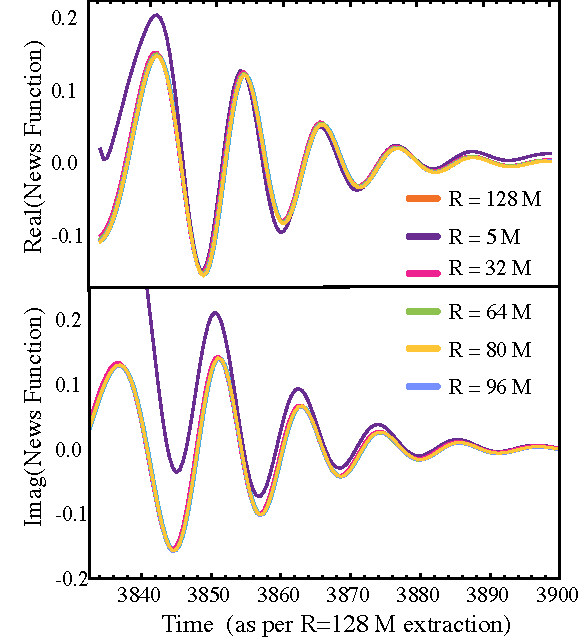
\includegraphics[width=0.5\textwidth]{AlignmentPlot_orig.pdf} } 
\subfloat{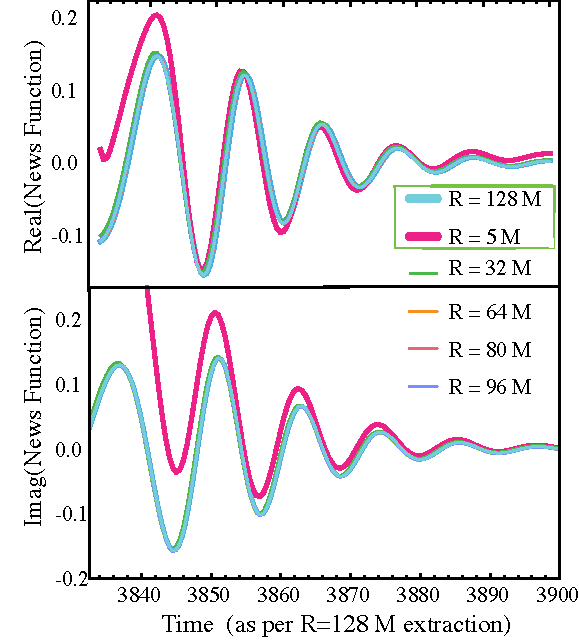
\includegraphics[width=0.6\textwidth]{figures/AlignmentPlot_refreereport_2.pdf} }
%\subfloat{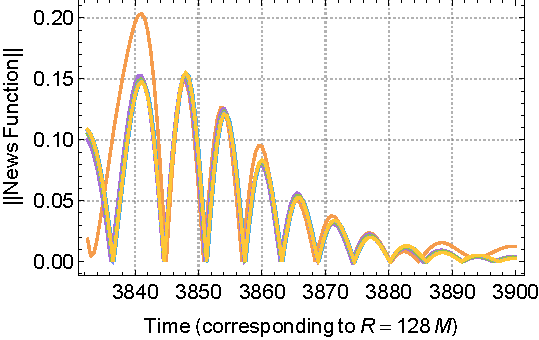
\includegraphics[width=0.45\textwidth, height=5.5cm]{AbsGlobalPeaksAlignedPlot.pdf} }
\caption{The $l=m=2$ mode of the news function seen at $\fni$ extracted from worldtube boundaries of $R = 5\,M$,~$32\,M$,~$64\,M$,~$80\,M$, ~$96\,M$~and~$128\,M$.  The horizontal axis corresponds to the time stamps associated with the news function corresponding to CCE from $R = 128\,M$. The \textbf{top panel} shows the real part and the \textbf{bottom panel} shows the imaginary part of the news function. The alignment of news functions has been done such that the overlap is maximized. The transformation that changes the gauge from a non-inertial to an inertial observer has not been applied to any of the extractions. All of the extractions beginning with $R = 32\,M$ seem to agree with one another (to the point of overlapping with the $R = 128\,M$ line). Notice that the amplitude of the news function extracted from $R = 5\,M$ deviates from the other extractions, especially in the first cycle. Nevertheless, the phase evolution between the news function from extraction radii seem to agree. The primary goal of this figure is to compare the extracted waveforms at $R = 5\,M$ and $R = 128\,M$. Thus we have bolded and boxed these lines.}
\label{fig:AlignmentAtMaximumOftheNews}
\end{figure*}
}






\newcommand{\PsiFourComparisonFigure}{%
\begin{figure*}[!htbp]
\subfloat{\includegraphics[width=0.7\columnwidth, keepaspectratio]{figures/Psi4Ref.pdf}}
\caption{$\Psi_4$ in on the x-axis (in the equatorial plane) for both a single BH with an $l=m=2$ perturbation of amplitude $\varepsilon = 7.5 \times 10^{-3}$ (\textbf{top panel}) and $\varepsilon = 10^{-3}$ (\textbf{bottom panel}), and for the BBH ringdown at times that achieve the same Kerrness. For all cases, Kerrness is matched on a coordinate 2-sphere of $R=5\,M$. The x-axis of the plot shows the radius, and includes the data within the Gaussian envelope of width $R=8\,M$, as described in Fig.~\ref{fig:Envelopes}. Note that this is only meant to show qualitative agreement between $\Psi_4$ on both slices, as the quantity is still subject to coordinate tetrad effects in the strong-field region. Notice that although the two systems look similar, the mapping does have some imperfections. Recall, however, that it is ultimately the invariant Kerrness measures that determine the mapping between the perturbation amplitude and the BBH merger-ringdown time.}
\label{fig:Psi4Comparison}
\end{figure*}
}





\newcommand{\spread}{%
\begin{figure}[!htbp]
\subfloat{\includegraphics[width=\columnwidth, keepaspectratio]{figures/spread.pdf}}
\caption{Spread in estimation of dominant mode frequency as a function of SNR. We present the spread, $\sigma_{f}$ in the estimation of frequency calculated using Fisher information matrix formalism. We should the increase in spread with decreasing SNR, providing the rough intuition on the implication of Fig.~\ref{fig:PercentageSNR} on parameter estimation.}
\label{fig:spread}
\end{figure}}



\newcommand{\postItSpecial}{%
\begin{figure*}[!htbp]
\subfloat{\includegraphics[width=\columnwidth,keepaspectratio]{figures/A0_percentSp.pdf} }
\caption{This figure is similar to Fig.~\ref{fig:PostItPanel} but for Speciality Index. We plot this separately as it is an independent measure and decays rapidly compared to the other measures. Further, we do not indicate the $1\%$ of peak line because of numerical noise (cf. Fig.~\ref{fig:Rainbow}) which leads to unreliable root finding for time of percentage decrease.}
\label{fig:specialityIndex}
\end{figure*}}

\newcommand{\perOnWave}{%
\begin{figure*}
\subfloat{\includegraphics[width=\textwidth,keepaspectratio]{figures/ampmap_withoutspec_tight_withamp.pdf} }   
\caption{The concomitant decrease of all of our Kerrness measures. The dashed lines indicate the time at which all the measures decay to at least the indicated $\%$ of peak. The bands color the region in which different measures decrease to the indicated $\%$ of peak. Notice that there is about half a cycle spread in each of these bands. Therefore, the dashed lines provide a conservative idea of the validity of the choice of the start time for data analysis. We have specifically included the spread of these bands as a quantifier of error bounds in the statements of validity made further in this chapter. Furthermore, one could shrink the right boundary of these shaded bands if one combines the Kerrness measures with appropriate weights based on their sensitivity to the spacetime curvature and the final remnant's effective potential. }
\label{fig:PercentOnTheWave}
\end{figure*}
}

\newcommand{\ampmap}{%
\begin{figure}[!htbp]
\subfloat{\includegraphics[width=0.7\columnwidth, keepaspectratio]{figures/amplitude_mapping.pdf}}
\caption{Mapping the inferred perturbation amplitude close to the BH onto the news function. The \textbf{top panel} shows the spread in the crossing times computed using just the Speciality Index, the \textbf{middle panel} uses only the algebraic measures and the \textbf{bottom panel} utilizes only the geometric measures. Notice that amplitudes larger than $2 \times 10^{-3}$ do cross the post-merger timeslices when computed using the geometric measures and that the crossing time spreads in them are relatively large, suggesting a difference in the symmetry of a perturbed Kerr metric and the post-merger BBH spacetime. However, this does not seem to be reflected when we just consider the algebraic measures as they have a relatively small spread in the crossing time. The spread in the crossing time of the Speciality Index is equal to the sampling rate.}
\label{fig:crossingtime}
\end{figure}}

\newcommand{\SNRdp}{%
\begin{figure}[!htbp]
\subfloat{\includegraphics[width=0.7\columnwidth, keepaspectratio]{figures/SNR_Erad_fixed.pdf} } 
\caption{The\textbf{ top panel} of this figure shows the percentage decrease of SNR from the peak value. The $\%$ SNR is set to $100$ at $t_{\mathrm{merger}}$. For this plot, we evaluate Eq.~\eqref{eq:SNR} with varying lower bounds for the integration. The dashed horizontal lines correspond to $\{80, 60, 40, 20\} \%$ SNR. On the same plot, we mark the perturbation amplitude bands for a direct comparison between perturbation amplitude and statistical error. Notice that by the time the perturbation amplitude near the BH decreases by an order of magnitude, there is only a few percent of SNR left in the signal, emphasizing the sharp trade-off between the systematic biases arising from modeling the post-merger as perturbed Kerr and the statistical uncertainty arising due to exponentially decay of signal amplitude.  The \textbf{bottom panel} shows the total energy radiated in units of $M$ during the merger-ringdown. This is calculated by integrating Eq.~\eqref{eq:EnergyRad}. Again, we have plotted the concomitant percentage decrease of the Kerrness measures from their peak values for an easy comparison between the statistical and systematic errors associated with the choice of the start time of ringdown. In particular, the constant settling in the total radiated energy occurs between the time when the Kerrness measures have decayed to $5-1 \%$ of their peak values, implying that at these times the GW is very weak in amplitude.  }
\label{fig:PercentageSNR}
\end{figure}
}




\newcommand{\postIt}{%
\begin{figure*}
\subfloat{\includegraphics[width=0.5\textwidth]{figures/A0_percentD1.pdf} }
\subfloat{\includegraphics[width=0.5\textwidth]{figures/A0_percentD3.pdf} }  \\[-0.3cm]
\subfloat{\includegraphics[width=0.5\textwidth]{figures/A0_percentD2.pdf} }
\subfloat{\includegraphics[width=0.5\textwidth]{figures/A0_percentK1.pdf} }
\caption{Connecting the Kerrness measures in the strong-field to dynamics at $\fni$ using the procedure described in Sec.~\ref{sec:AFQ_implementation} on the BBH post-merger. The \textbf{left panels} map the algebraic measures and the \textbf{right panels} map the geometric measures on to the news function. The \textbf{top panel} within each subplot corresponds to a Kerrness measure in the strong-field, while the \textbf{bottom panel} shows the news function at $\fni$. The purpose of plotting the news function directly below each Kerrness measure is to emphasize that the top and bottom panels are mapped to the same time axis. The dashed lines of different colors indicate the $\%$ decrease from the peak value of the respective Kerrness measures. The horizontal axis corresponds to the simulation coordinate time induced on the news function extracted from a world tube radius of $R=128\,M$. Furthermore, unlike the strong-field result plots that aim at rigorous characterization of isometry to Kerr, here we aim at providing insight into validating the start time of ringdown for data analysis. Therefore, these plots are on linear scale as opposed to logarithmic scale. Notice that the curves on the left panel decay more slowly than those on the right; Type D 1 is the slowest to decay, closely followed by Type D 2. Also, recall that we cannot compare the magnitude of the top part of each of these panels as they are dimensionally different. }
\label{fig:PostItPanel}
\end{figure*}}

\newcommand{\phiplot}{%
\begin{figure}[!htbp] \subfloat{\includegraphics[width=\columnwidth]{figures/phase_differi.pdf} } 
\caption{The phase discrepancy between the news function extracted from a worldtube radius of $R=5\,M$ and $R= 128\,M$. The news functions are aligned to maximize the overlap. The \textbf{top panel} presents the phase evolution of the news function for each extraction radius. The \textbf{bottom panel} shows the fractional difference defined as $\phi_{128} - \phi_{5}$. Notice that the phase difference is significant at the very beginning but quickly decreases to an acceptable level for our analysis. We notice that the phase difference oscillates about 1 radian, indicating the level of error we introduce by - a) not performing the final gauge transformation, b) imposing no-ingoing condition for CCE.  }
\label{fig:phasediffcomb}
\end{figure}}

\newcommand{\cartoon}{%
\begin{figure}[!htbp]
\centering
\subfloat{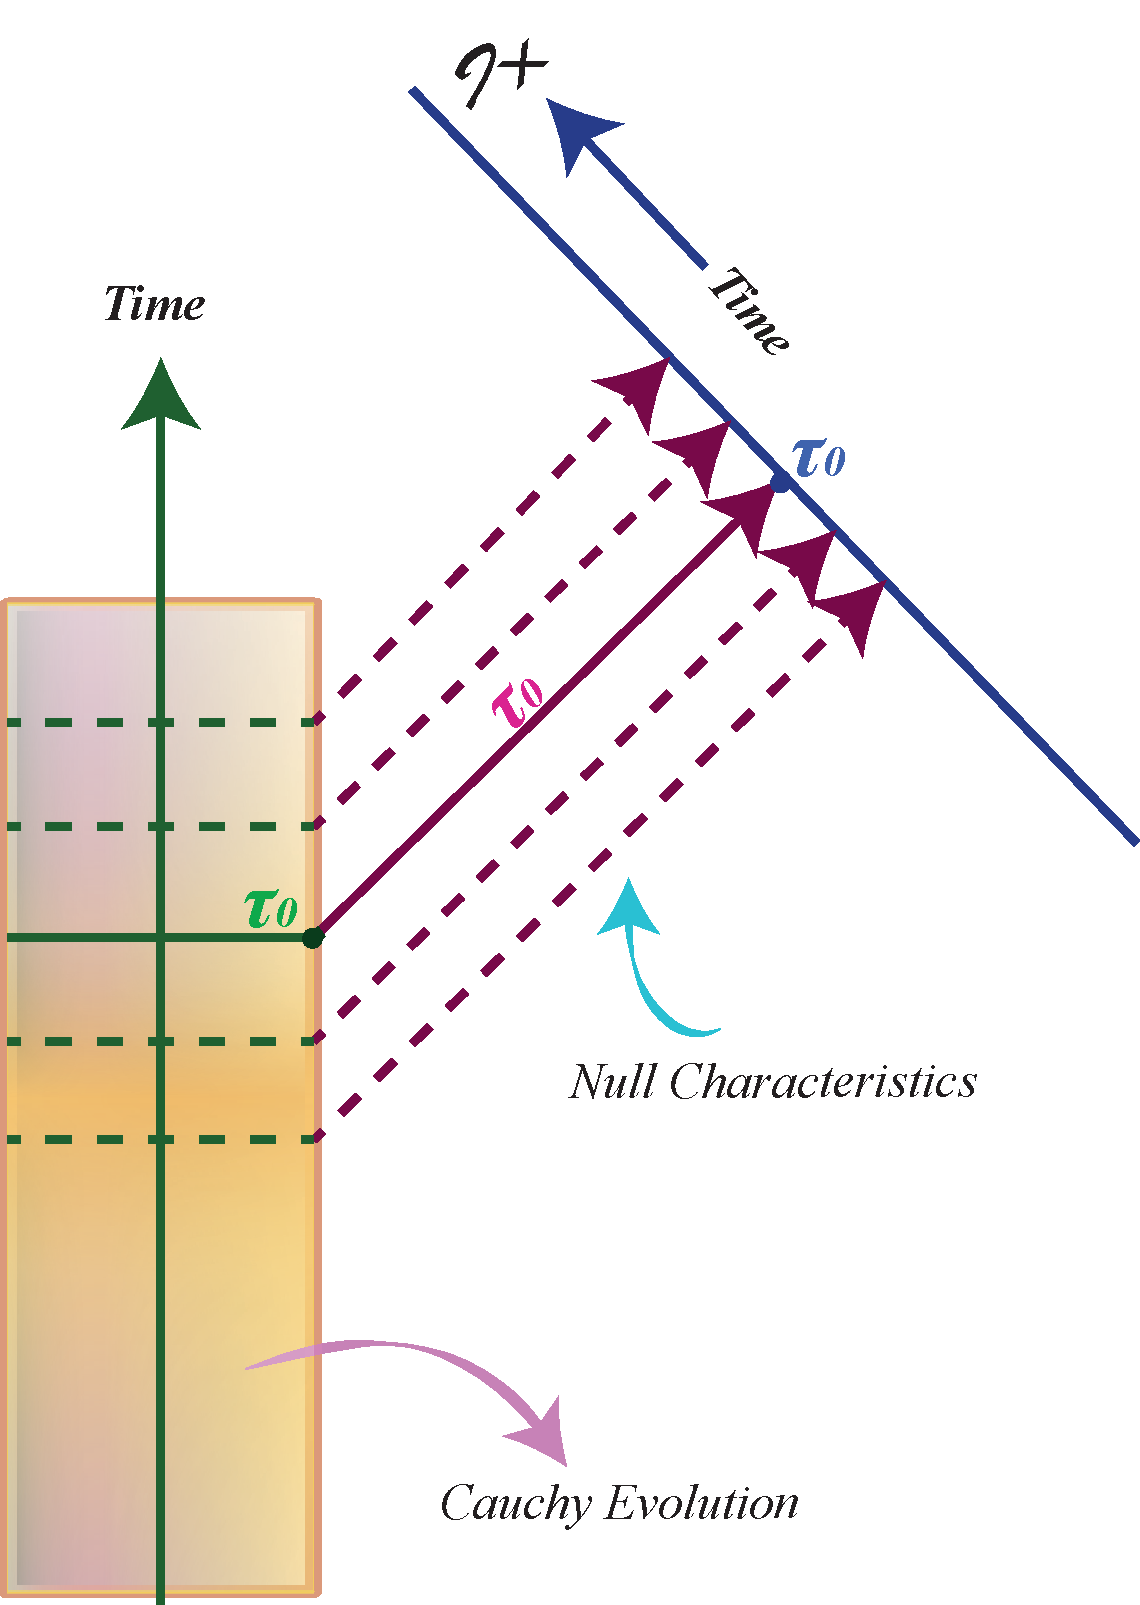
\includegraphics[width=0.7\columnwidth]{figures/Cartoon_Kerrness1.pdf} }
\caption{Prescription for connecting the strong-field information to the asymptotic frame dynamics. The colored cylinder represents the region of spacetime that is evolved by the Cauchy code. The vertical green line within the cylinder indicates the direction of coordinate time. The horizontal lines represent time slices. The details of the location of time slices depend on the gauge choice. The pink boundary of the cylinder depicts the worldtube from where the CCE is performed. The purple lines with unit slope illustrate the null characteristics along which the information on the worldtube is propagated to (the solid blue line) $\fni$. In our procedure of associating information in the source frame with the asymptotic frame, we identify all the points along a characteristic by an equivalence. The solid green line in the cylinder acts as a source to the waveform feature at $\tau_0$ observed at $\fni$.}
\label{fig:Cartoon}
\end{figure}
}

\newcommand{\tgr}{% 
\begin{figure}[!htbp]\subfloat{\includegraphics[width=\columnwidth]{figures/CombinedTGR.pdf} } 
\caption{Comparison of the times chosen in the testing GR study of GW150914~\cite{TheLIGOScientific:2016src}. Here, we make statements about their validity to perform tests that rely on the perturbative nature of the BH. Specifically, we propose that a plot of this nature be done for future detections, especially if the SNR is high, to gain an insight into the inferred strong-field perturbation amplitudes corresponding to different choices of ringdown start time. The dotted line in the \textbf{top panel} shows different choices of start time for performing tests on the detector data. The \textbf{bottom panel} shows what each time choice corresponds to in the simulation gauge. Although a practical choice of start time to perform tests like no-hair theorem tests should be decided based on the interplay between the statistical and systematic uncertainty, a plot of this nature gives significant understanding of the results of such tests. For instance, in the case of GW150914, had the signal been much louder than what we observed, this plot suggests that we \textit{could} get biased results due to large inferred perturbation amplitude in the strong-field leading to errors in modeling the post-merger as a perturbed BH at 3 ms.}
\label{fig:TGR}
\end{figure}
}

\newcommand{\ConvergenceTestFigure}{%
\begin{figure}[!htbp]
\subfloat{\includegraphics[width=0.85\textwidth]{figures/SingleBHConvergenceAbsolute.pdf} } 
\caption{Convergence of Kerrness measures on a numerical BH in Kerr-Schild coordinates with 
dimensionless spin $\chi = (0.2, 0.3, 0.4)$. We observe exponential convergence towards the theoretical value of zero with numerical resolution. For each measure $\zeta$, we present $\|\zeta\|/\|\zeta_0\|$, the L2 norm over the spatial slice normalized by the L2 norm of the lowest resolution. The resolution is expressed $\sqrt[3]{N}$, where $N$ is the number of spectral collocation points in the domain.
  %%\note{MS: remove 'Subdomain' from the horizontal axis label.
%    Also, perhaps plot vs cube root of $N$, where $N$ is the total number of
%    collocation points?  Then you don't need to explain radial/angular basis
 % functions.}
}
\label{fig:ConvergenceTest}
\end{figure}
}

\newcommand{\EnvelopesFigure}{%
\begin{figure}[!htbp]
\subfloat{\includegraphics[width=\columnwidth]{figures/Envelopes.pdf} } 
\caption{Envelope function from Eq.~\eqref{eq:envelope}, for two choices of width and falloff parameters, $\{W, F\}$. We show how the envelope parameters affect an  extraction radius of $R=5\,M$ (marked by the dashed black line). For our chosen values of $\{W = 6\,M, F = 8\}$, the envelope is at $\sim 1$ and $R=5\,M$, while for $\{W = 3\,M, F = 8\}$, the envelope affects the perturbation amplitude at $R=5\,M$. We have checked that using a smaller envelope does not change the qualitative behavior of our results.}
\label{fig:Envelopes}
\end{figure}
}

\newcommand{\KerrPertAmplitudeFigure}{%
\begin{figure}[!htbp]
\subfloat{\includegraphics[width=\columnwidth]{figures/KerrPertAmplitude.pdf} } 
\caption{Behavior of absolute Kerrness measures with perturbation amplitude $\varepsilon$. We compute this on an $l=m=2$ QNM perturbed Kerr BH with the same mass and spin as the final remnant in the BBH simulation we consider in this chapter. We average each measure on a coordinate 2-sphere of $R=5\,M$. Note that we do not plot Type D 4 due to the high level of numerical noise in the measure, but it behaves similarly to Type D 3. The behavior is initially quadratic with $\varepsilon$ for all measures. At larger amplitudes $\varepsilon \geq 5 \times 10^{-3}$, Type D 2, D 3, D 4 and Kerr 1 show higher-power dependence, and hence non-linearity. We show this  $\varepsilon_\mathrm{crit} \sim 5 \times 10^{-3}$ by a dashed vertical line. The lines between the points are only used to visually connect them (rather than being fits).
}
\label{fig:KerrPertAmplitude}
\end{figure}
}


\newcommand{\HorizonDataFigure}{%
\begin{figure}[!htbp]
\subfloat{\includegraphics[width=0.7\columnwidth]{figures/HorizonData.pdf} } 
\caption{Settling of the post-merger AH as a function of coordinate time. The \textbf{top panel} shows the areal mass quickly attaining a constant value and the minimum and maximum radii $R$ of the horizon exponentially settling to final values. Each quantity $\zeta$ is presented as $|\zeta  - \zeta_\mathrm{final} |/\zeta_\mathrm{final}$ where $\zeta_\mathrm{final}$ is the value at the final time of the simulation. The \textbf{bottom panel} shows the behavior of the initially excited AH mass multipoles, labeled by the $l_\mathrm{eff}$ given in Eq.~\eqref{eq:leff} at the final time. The initially excited quadruple moments ($l_\mathrm{eff} \sim 2$) are shown by the dashed lines, while the initially excited hexadecupole moments ($l_\mathrm{eff} \sim 4$) are shown by the solid lines. As discussed in the text, two of the quadropule moments and four of the hexadecupole moments, as well as the $l \sim 1$ and $l \sim 3$ moments immediately vanish due to symmetry. Thus, we do not plot them in this figure. The excited multipoles either exponentially decay or reach constant values consistent with the values expected for Kerr~\cite{Owen:2009sb}.
}
\label{fig:HorizonData}
\end{figure}
}

\newcommand{\RainbowFigure}{%
\begin{figure*}
\subfloat{\includegraphics[width=\textwidth]{figures/RainbowPlotAbs.pdf} } 
\caption{Behavior of absolute Kerrness measures with coordinate time on BBH post-merger spacetime. The measures are averaged on a variety of concentric nested coordinate 2-spheres of radii $R$ around the BH, as indicated by the colors. Larger values \textit{within each subplot} mean that the 2-sphere is farther from being locally isometric to Kerr. For measures that involve higher-order numerical derivatives, we present the results only at radii  where they are at least somewhat well resolved. All plots, however, include $R = 5\,M$, the radius we use to map Kerrness onto the waveform. Type D 4 is particularly noisy, as it contains the highest number of numerical derivatives. The measures exponentially decay as the spacetime approaches Kerr, ultimately reaching a numerical noise floor. We observe that the peak of each measure moves outwards with radius, indicating propagation of non-Kerrness.}
\label{fig:Rainbow}
\end{figure*}
}

\newcommand{\NoiseFloorFigure}{%
\begin{figure}[!htbp]
\includegraphics[width=\columnwidth]{figures/SimulationNoiseConvergence.pdf}
\caption{Exponential convergence of the noise floor of each Kerrness measure on the final timestep of the BBH simulation. Each measure $\zeta$ is presented as an average over a 2-sphere of $R=5\,M$ (where the measures have settled to a noise floor), normalized by $|\zeta_0|$, the average of the lowest resolution. The resolution is indicated by $\sqrt[3]{N}$, where $N$ is the number of spectral collocation points. The convergence to zero shows that the  noise floor observed in Fig.~\ref{fig:Rainbow} is a numerical noise floor, rather than real a physical artifact. We have also testing this convergence behavior on a 2-sphere $R=5\,M$ and verified that the behavior is consistent (although more noisy).}
\label{fig:NoiseFloor}
\end{figure}
}

\newcommand{\KerrTwoFigure}{%
\begin{figure}[!htbp]
\subfloat{\includegraphics[width=\columnwidth]{figures/RainbowPlotKerr2Abs.pdf} } 
\caption{Kerr 2 measure throughout the post-merger BBH simulation, averaged on a variety of coordinate 2-spheres of radius $R$. The values remain relatively constant and low, indicating that no NUT charge is gained during ringdown.}
\label{fig:KerrTwo}
\end{figure}
}

\newcommand{\SwirlFigure}{%
\begin{figure*}
\subfloat{\includegraphics[width=0.7\textwidth]{figures/Swirl100.png} } \\[-0.01cm]
%\subfloat{\includegraphics[width=\textwidth, height=0.15\textheight]{Swirl50.png} } \\[-0.05cm]
\subfloat{\includegraphics[width=0.7\textwidth]{figures/Swirl30.png} } \\[-0.01cm]
\subfloat{\includegraphics[width=0.7\textwidth]{figures/Swirl10.png} } \\[-0.01cm]
%\subfloat{\includegraphics[width=\textwidth, height=0.15\textheight]{Swirl5.png} } \\[-0.05cm]
\subfloat{\includegraphics[width=0.7\textwidth]{figures/Swirl1.png} } \\[-0.01cm]
\caption{Absolute Kerrness measures on slices of the BBH post-merger spacetime. The data is presented in the equatorial plane, with the gray region corresponding to the excised BH. The black circles correspond to coordinate radii $R=5\,M$ and $R=10\,M$. The columns correspond to Speciality Index, Type D 1, and Kerr 1, and the rows (from top to bottom) correspond to coordinate times at which the each measure at $R=5\,M$ achieves $100\%$, $30\%$, $10\%$, and $1\%$ of the combined peak value.  The quadrupolar pattern (with $|m| = 2$) in all three measures is consistent with the dominant quadrupolar radiation (recall that these are absolute measures, and hence do not distinguish between positive and negative values). Notice that the algebraic measures---Speciality Index and Type D 1---settle outward-in, whereas Kerr 1, a geometric measure, settles inward-out. Additionally, the structures in the measures are visible even at $1\%$ of the peak value. We can compare these measures to $\Psi_4$ (in Figs.~\ref{fig:Psi4Comparison}) to infer their sensitivity to the spacetime curvature features.}
\label{fig:Swirl}
\end{figure*}
}

%\Mark{\sout{the BBH post-merger slices and the $l=m=2$ perturbed Kerr metric (\textbf{b} and \textbf{d}), for }}
%\Mark{\sout{We plot $\Psi_4$ on the BBH simulation at these times in subfigures \textbf{b} and \textbf{d}.}} 
%\Mark{\sout{We plot $\Psi_4$ on the perturbed metrics in the x-y plane in subfigures \textbf{a} and \textbf{c}. We estimate the average times at which the slices achieve the same level of Kerrness as the perturbed metrics} 


\newcommand{\PsiFourComparisonFigureOld}{%
\begin{figure*}[!htbp] 
\subfloat[$\Psi_4$ on $\varepsilon = 7.5 \times 10^{-3}$ single BH]{\includegraphics[width=0.5\columnwidth]{figures/emTotal1A.png} \label{fig:psi41A}}
\subfloat[$\Psi_4$  for BBH at $\varepsilon = 7.5 \times 10^{-3}$ crossing time]{\includegraphics[width=0.5\columnwidth]{figures/emTotal1B.png} \label{fig:psi41B}}\\ [-0.3 cm]
\subfloat[$\Psi_4$ on $\varepsilon = 10^{-3}$ single BH]{\includegraphics[width=0.5\columnwidth]{figures/emTotal2A.png} \label{fig:psi42A}}
\subfloat[$\Psi_4$ for BBH at $\varepsilon = 10^{-3}$ crossing time]{\includegraphics[width=0.5\columnwidth]{figures/emTotal2B.png} \label{fig:psi42B} }
\caption{$\Psi_4$ in the equatorial plane for both a single BH with an $l=m=2$ perturbation of amplitude $\varepsilon = 7.5 \times 10^{-3}$ and $\varepsilon = 10^{-3}$ (\textbf{left panel}), and for the BBH ringdown (\textbf{right panel}) at times that achieve the same Kerrness as (\textbf{left panel}). For all cases, Kerrness is matched on a coordinate 2-sphere of $R=5\,M$. The two black circles correspond to coordinate radii $R=5\,M$ and $R=8\,M$. The Gaussian envelope of width $R=8\,M$, as described in Fig.~\ref{fig:Envelopes}, can be seen in the plots for the single BH cases. Note that this is only meant to show qualitative agreement between $\Psi_4$ on both slices, as the quantity is still subject to coordinate tetrad effects in the strong-field region. Notice that although the two systems look similar, allowing us to infer the BBH simulation perturbation amplitude, the mapping does have some imperfections.
}
\label{fig:Psi4ComparisonOld}
\end{figure*}
}

\newcommand{\CrossingTimeFigure}{%
\begin{figure*}
\subfloat{\includegraphics[width=\textwidth]{figures/PerturbationPlot5BetterData.pdf} } 
\caption{
Comparison of the Kerrness measures during the BBH post-merger to the values of the Kerrness measures on an $l=m=2$ QNM perturbed Kerr BH of various perturbation amplitudes $\varepsilon$, with the same mass and spin parameters. The measures are averaged on a 2-sphere of coordinate radius $R=5\,M$, which corresponds to comparable areal radii of $\sim 2.59\,M$ in both systems. The measures evaluated on the BBH slices are shown by solid black lines, decaying as a function of time. The Kerrness measures for the perturbed metric are presented as horizontal dashed red lines, one for each $\varepsilon$. The times at which the BBH curves intersect the Kerrness values for a given $\varepsilon$ Kerr perturbation give a scale for the BBH Kerrness measures as the post-merger progresses. These times, known as \textit{crossing times} are then mapped onto the waveform, and used to validate the start time of ringdown. Note that the measures have different crossing times. The time axes are shifted to agree with the timestamps of the GW at $R= 128\,M$, as explained in Table~\ref{tab:Tshift}.
}
\label{fig:CrossingTime}
\end{figure*}
}

\newcommand{\StrainsFigure}{%
\begin{figure}[!htbp]
\subfloat{\includegraphics[width=\columnwidth]{figures/Strains.pdf} } 
\caption{Comparison between the strain $h$ calculated using CCE and RWZ methods. All waveforms are presented in terms of the $l=m=2$ mode. We use the fact that the strain is the integral of the news function to cross-check the methods. The \textbf{top panel} shows the CCE news function $\mathcal{N}_\mathrm{CCE}$ compared to $\dot{h}_\mathrm{RWZ}$, the derivative of the RWZ strain. The \textbf{bottom panel} shows $h_\mathrm{CCE}$, the integral of the CCE news function, compared to the RWZ strain $h_\mathrm{RWZ}$. We find good agreement until late times, when $h_\mathrm{CCE}$ begins to drift, likely due to the numerical integration scheme used.}
\label{fig:Strains}
\end{figure}
}

\newcommand{\Msun}{\ensuremath{\mathrm{M}_\odot}}
\newcommand\perMpcyr{\ensuremath{\mathrm{Mpc}^{-3}\,\mathrm{y}^{-1}}}
\def\dogTrialFAR{1 in $4 \times 10^{4}$\,y}
\def\dogFAR{1 in $7\,000$\,y}
\def\dogTrialFAP{\ensuremath{3 \times 10^{-6}}}
\def\dogFAP{\ensuremath{7 \times 10^{-5}}}
\def\dogTime{2010 September 16, 06:42:23 UTC}
\def\dogChirp{between $4.4$ and $5.2\,\Msun$}
\def\dogEta{$0.16 \le \eta \le 0.25$}
\def\dogDist{between $7$ and $60$\,Mpc}
\def\dogSNR{\ensuremath{\rho_c = 12.5}}
\def\SOURCE{\bf{SOURCE}}
\def\MASSONE{M1 \Msun}
\def\MASSTWO{M2 \Msun}
\def\DISTANCE{D Mpc}
\def\FAR{N yr$^{-1}$}
\def\START{MONTH, DAY, YEAR}
\def\STOP{MONTH, DAY, YEAR}
\def\TIME{GPS}

\newcommand{\Caltech}{\affiliation{Theoretical Astrophysics,
    Walter Burke Institute for Theoretical Physics,\\
    California Institute of Technology, Pasadena, California 91125, USA}}
\newcommand{\Cornell}{\affiliation{Center for Radiophysics and Space
    Research, Cornell University, Ithaca, New York 14853, USA}}
\newcommand{\Syracuse}{\affiliation{Syracuse University, Syracuse, NY 13244, USA}}



%The final stage of a binary black hole merger is ringdown, in which the system is described by a Kerr black hole with quasinormal mode perturbations. It is far from straightforward to identify the time at which the ringdown begins. Yet determining this time is important for precision tests of the general theory of relativity that compare an observed signal with quasinormal mode descriptions of the ringdown, such as tests of the no-hair theorem. We present an algorithmic method to analyze the choice of ringdown start time in the observed waveform. This talk will outine the theoretical framework used in this analysis, and the following talk, ``On choosing the start time of binary black hole ringdown II: Results'', will discuss the results.  This method is based on determining how close the strong field is to a Kerr black hole (\textit{Kerrness}). Using numerical relativity simulations, we characterize the Kerrness of the strong-field region close to the black hole using a set of local, gauge-invariant geometric and algebraic conditions that measure local isometry to Kerr. We produce a map that associates each time in the gravitational waveform with a value of each of these Kerrness measures; this map is produced by following outgoing null characteristics from the strong and near-field regions to the wave zone.

%On choosing the start time of binary black hole ringdown II: Results

%The final stage of a binary black hole merger is ringdown, in which the system is described by a Kerr black hole with quasinormal mode perturbations. It is far from straightforward to identify the time at which the ringdown begins. Yet determining this time is important for precision tests of the general theory of relativity that compare an observed signal with quasinormal mode descriptions of the ringdown, such as tests of the no-hair theorem. We present an algorithmic method to analyze the choice of ringdown start time in the observed waveform. This talk will discuss the results of applying the framework outlined in the previous talk, ``On choosing the start time of binary black hole ringdown I: Theory'' on a numerical relativity simulation with parameters consistent with GW150914 - the first gravitational wave detection. We find that the choice of ringdown start time of $3\,\mathrm{ms}$ after merger used in the GW150914 study to test general relativity corresponds to a high dimensionless perturbation amplitude of $ \sim 7.5 \times 10^{-3}$ in the strong-field region. This suggests that in higher signal-to-noise detections, one would need to start analyzing the signal at a later time for studies that depend on the validity of black hole perturbation theory.

\section{Introduction}
%% QNM introduction, Overall goal as motivated by the fact that we can do LIGO data analysis, no-hair theorem 

The quasi-normal mode (QNM) spectrum seen during the ringdown of a perturbed black hole (BH) is determined by the Teukolsky equation; it carries the signature of the BH potential along with the BH horizon and asymptotic boundary conditions~\cite{Teukolsky1, Teukolsky2, Teukolsky3}. The recent detections of binary black hole (BBH) gravitational wave (GW) signals by LIGO (the Laser Interferometer Gravitational-Wave Observatory)~\cite{Abbott:2016blz, Abbott:2016nmj, TheLIGOScientific:2016pea, Abbott:2017vtc, PhysRevLett.119.141101} allow us to begin to probe this QNM signature~\cite{TheLIGOScientific:2016src}. The QNM spectrum in a gravitational-wave observation allows us to perform tests of the no-hair theorem. This theorem states that vacuum, asymptotically flat, stationary, axisymmetric, uncharged BHs are completely characterized by two parameters: the mass and the spin~\cite{Mazur:2000pn,misner1973gravitation,Dreyer,Gossan,Kamaretsos}. This allows us to constrain modified theories of gravity that violate the no-hair theorem~\cite{Berti:2015itd, Yunes:2016jcc}. Observing the QNM spectrum in GWs can be used to validate the BH uniqueness theorem. This theorem states that the exterior geometry of an vacuum, asymptotically flat, stationary, axisymmetric, uncharged BH must be Kerr~\cite{Mazur:2000pn, Mars:1999yn}. 

%% Testing GR, Choices of start time and that not motivated by source frame

%%\note{MS: It's not only the perturbative regime, right?  These perturbations must be QNM perturbations. Maybe this can be reworded slightly.} \swetha{[SB and MO: Are you referring to the tail effects in BH perturbation here?]}%\note{MS: I was thinking more of initial transients, which may not have gone away soon after merger.}

However, testing the no-hair and uniqueness theorems relies on observing GWs from the QNM perturbative regime (without additional transients remaining from the inspiral). This requires an appropriate choice of start time of this regime.\footnote{While conventions in the literature vary, in this chapter, by `ringdown', we explicitly mean the part of the post-merger gravitational waveform that can be described in terms of QNMs.} Identifying this time in the signal is mathematically an ill-defined problem, since QNMs form an incomplete and non-orthogonal basis~\cite{QNMincomplete,QNMnonorthogonal}. Hence, the conventions for choosing the start time of the ringdown have varied in the literature. Berti et al.~\cite{EMOP} and Baibhav et al.~\cite{Baibhav:2017jhs} chose the start time based on maximizing the energy contained in the QNM. London et al.~\cite{London} used $10\,M$ after the peak of the dominant mode of $\Psi_4$ (the Newman-Penrose scalar that encodes outgoing radiation) for fitting to NR waveforms.\footnote{ \label{note1} Since vacuum GR is a scale-invariant theory, it is convenient to express distance and time in terms of source mass by setting $G=c=1$. Explicitly, $ 1~M = M_{\mathrm{BH}} \times G/c^{3} ~\mathrm{seconds}$, where $M_{\mathrm{BH}}$ is the mass of the BH.} Kamaretsos et al.~\cite{2012PhRvL.109n1102K} chose $10\,M$ after the peak luminosity of the dominant mode of the waveform, while Thrane et al.~\cite{Thrane} proposed a loudness-dependent start time. In the  GW150914 testing general relativity (GR) chapter~\cite{TheLIGOScientific:2016src}, different start times were used to perform the QNM analysis shown in Fig.~5 of that chapter, and the results were consistent with GR when the start time was picked as $3~\mathrm{ms}$ (or later) after the merger.


%% We present an algorithmic way
None of these methods use information from the strong field to motivate the start times. The strong field refers to the region near the BHs (typically within a radius of few $M$), where the scale of the curvature is much smaller than the wavelength of a gravitational wave. In this chapter, we develop an algorithmic method for validating choices of the start time of ringdown using strong-field features. Specifically, we measure the \textit{Kerrness}, or closeness to Kerr, in the strong-field region of an NR simulation ringdown, and use null characteristics to map Kerrness onto the GW at asymptotic future null infinity, $\fni$. We then demonstrate this method on a GW150914-like system. However, this method is generic, and this procedure can be carried out for any BBH system.

% %\note{MS: Is 'source frame' the right phrase?  Would 'strong-field regime' or 'near zone' be better?  I always thought 'source frame' meant 'coordinate system with the source at the origin', to distinguish from 'detector frame' which is where LIGO is.  The transformation between these frames involves the rotation of the earth and its motion about the sun, etc.} 

%% Introduce why finding Kerrness in the source frame is non-trivial. and previous studies 
Determining Kerrness in the strong-field regime is non-trivial, since one needs a coordinate-invariant way of identifying a metric as Kerr. Necessary and sufficient conditions for a gauge-invariant characterization of local isometry to a Kerr manifold were proposed by Garc\'{i}a-Parrado G\'{o}mez-Lobo in~\cite{lobo16}.\footnote{Throughout this text, \textit{isometry} refers to the smooth mapping of manifolds equipped with metrics.} We use this set of algebraic and geometric conditions to provide a numerical measure of Kerrness. Previous studies have used multipole moments of the BH apparent horizon~\cite{Owen:2009sb}, horizon spin measurement comparisons~\cite{Scheel:2008rj}, or Petrov classification~\cite{Baker,Campanelli:2008dv,Owen:2010vw} to characterize ringdown spacetimes. Our work is the first set of conditions that completely characterizes a spacetime as isometric to a Kerr manifold. We study the violation of these conditions post-merger in the strong field of a BBH simulation.

%% Why connecting source to asymptotic is non-trivial 
Connecting the strong-field region to the wave zone is a challenge, as the simulation gauge is different from the gauge in which GWs are observed. There is no straightforward way to transform between these gauges. Furthermore, establishing simultaneity between events is not possible in the GR framework, and thus there is no direct map between an event in the strong-field region and a point on the waveform. We therefore devise a scheme to approximately associate the two frames. The association used in this study is of a cause-effect nature: we follow the outgoing null characteristics from the strong-field region to the wave zone using a Cauchy Characteristic Extraction scheme (CCE)~\cite{Handmer:2014qha, Handmer:2015dsa, Casey}, and associate events in the strong field to the wave zone. However, given that GR is a nonlinear theory, the source associated with a particular feature in the GW signal may not be well localized in the spacetime. Nevertheless, one would expect that the source dynamics that dominantly contribute to certain features in the waveform be localizable to a certain extent. Several such approximate localizations have been performed in linear perturbation theory~\cite{PriceAndPlunge,VitorsECO}. 

%% Roadmap
This chapter is organized as follows. Sec.~\ref{sec:Theory} presents the theoretical methods used in this chapter, and Sec.~\ref{sec:Implementation} discusses their implementation in NR simulations. Sec.~\ref{sec:ResultMain} then presents and discusses the results of applying these methods to an NR simulation with GW150914-like parameters. We conclude in Sec.~\ref{sec:Conclusion}. Figs.~\ref{fig:PercentOnTheWave} and~\ref{fig:TGR} are the flagship figures, presenting our major results. The the results are quantitatively summarized in Table~\ref{tab:combined info}.

%% Conventions
\subsubsection*{Conventions}
%\masha{SB + MO: Duncan wants to remove this header, but we think it's nice to single it out for people to refer to when reading the chapter}
We work with the standard 3+1 decomposition of NR (cf.~\cite{baumgarteShapiroBook} for an introduction). In this chapter, $g_{ab}$ refers to the spacetime metric, $n^a$ refers to the timelike unit normal vector, $\gamma_{ij}$ refers to the spatial metric on each slice, $D_i$ is the covariant derivative with respect to $\gamma_{ij}$, and $K_{ij}$ refers to the extrinsic curvature. We set $G = c = 1$ and express all quantities in terms of $M$, the sum of the Christodoulou Masses of the two BHs at the start of the simulation. Latin letters at the start of the alphabet, $\{a, b, c, d\}$, refer to (4-dimensional) spacetime indices, while Latin letters in the middle of the alphabet, $\{i,j,k,l,m,n\}$ are (3-dimensional) spatial indices. We denote complex conjugation by an overbar (e.g. $\bar{A}$). To avoid confusion among the multiple meanings of `data' in this chapter, we refer to the vacuum data $\{\gamma_{ij}, K_{ij}\}$ on a spatial slice simply as `a slice'.\footnote{\textit{Vacuum data} means that the spatial metric, $\gamma_{ij}$, and the extrinsic curvature $K_{ij}$ satisfy a set of constraint equations corresponding to the decomposition of the vacuum Einstein equations.} Similarly, rather than being purely geometric, a `slicing' in our case is a foliation equipped with a coordinate chart.


%We set $G = c = 1$ and express all quantities in code units%\note{MS: please remove the phrase 'code units'. In a chapter (unless the chapter is explicitly about details of the code), the units used in a particular code should be unimportant.}, given in terms of total
%\Mark{\sout{ADM} initial} %\note{MS: $M$ is the sum of the two Christodoulou Masses at $t=0$.  This is different than the ADM mass at $t=0$, but should agree (to good precision) with the ADM mass at $t=-\infty$.} mass $M$. 




\section{Theory}
\label{sec:Theory}
\subsection{Characterizing strong-field Kerrness}

\FlowChartFigure

%\masha{SB + MO: Duncan wants to ``make this a section, don't use subsubsubsections in PRD". We have written this chapter so that we have a section that contains pure theory valid for any system, and a section about numerical implementation (specific to the GW150914 system and the code) and a results + conclusion section}
%% Roadmap
First, we explain our method of measuring Kerrness in the strong-field region and develop a method to map it onto  $\fni$. Secs.~\ref{sec:KerrnessBackground}~and~\ref{sec:KerrnessTheory} discuss theoretically characterizing Kerrness in the strong-field region, while Secs.~\ref{sec:AFQMotivation},~\ref{sec:Challenges},~and~\ref{sec:AFQ_theory} discuss mapping strong-field information onto the wave zone via null characteristics. 

\subsubsection{Overview and historical background}
\label{sec:KerrnessBackground}
%% Paragraph about the overall goal in the source frame 
Our overall goal in this section is to evaluate \emph{Kerrness}: how close a numerical BH ringdown spacetime is to being locally isometric to the Kerr spacetime. In order to evaluate the Kerrness of a spacetime, we first need a set of theoretical conditions to evaluate whether a spacetime \textit{is} isometric to Kerr. We can then turn these conditions into a set of \textit{measures}, where deviation from zero indicates being farther from being locally isometric to Kerr. In a numerical simulation, one would evaluate these measures on spatial slices of a simulation. To characterize Kerrness in the strong-field region, one needs local quantifiers evaluated close to the BH, as opposed to looking at regions far away which are contaminated by gravitational radiation. Consequently, we seek a point-wise measure and do not use global measures on a slice such as those proposed in~\cite{Backdahl:2010cy,Backdahl:2010fa,Backdahl:2011np}.


%% Paragraph about speciality, type D
Uniquely characterizing a spacetime as Kerr has been historically challenging---until recently one could only classify spacetimes up to a Petrov type, which gives a weaker classification that admits several manifolds besides Kerr. The Petrov classification uses algebraic properties of the Weyl tensor $C_{abcd}$ based on the four principal null directions (PNDs), by solving the eigenbivector problem (cf.~\cite{stephani2009exact} for a review)
\begin{align}
\label{eq:eigenvalue}
\frac{1}{2} C^{ab}{}_{cd} X^{cd} = \lambda X^{ab}\,,
\end{align}
where eigenbivectors $X^{ab}_{(\alpha)}$ have eigenvalues $\lambda_{(\alpha)}$. The degeneracies of the PNDs give a unique algebraic classification of a spacetime. A spacetime with no repeated PNDs is fully general (Petrov Type I). A spacetime with at least one repeated PND is \textit{algebraically special}. The Kerr metric belongs to a particular class of algebraically special spacetimes, the set of type D spacetimes, which have two double PNDs. A necessary condition for the manifold to be locally isometric to Kerr is to be type D.

%tetrad choice effects
Campanelli et al.~\cite{Campanelli:2008dv} used this approach to analyze a numerical BBH ringdown. They determined the degeneracies between the PNDs by solving the eigenbivector problem and measuring the difference between eigenvalues. Their analysis found that the spacetime first numerically settled to type II, which has only one double PND, and then to type D. Owen~\cite{Owen:2010vw} later showed that this measure was sensitive to the choice of tetrad used to compute the Weyl scalars needed to solve the characteristic equation. He proposed a new measure, less-sensitive to the choice of tetrad, and showed that the spacetime settled to type D without first settling to type II.

% NUT parameter study by campanelli
A type D spacetime can then be shown to be locally isometric to Kerr through additional conditions. Kerr belongs to the Kerr-NUT subset of type D spacetimes. One needs to show that a spacetime is Kerr-NUT and then constrain the acceleration and the NUT parameters. We give more information on Kerr-NUT spacetimes and the various parameters in Appendix~\ref{appendix:KerrNUTParameters}. \saul{Ref.}~\cite{Campanelli:2008dv} investigated the asymptotic behavior of the acceleration and the NUT parameter on a BBH simulation and showed they were constrained to be those of Kerr. %\note{MS: too much detail about Kerr-NUT here?  Perhaps say only that one can evaluate the acceleration and NUT parameters to get Kerr, and leave the rest out.} \swetha{SB + MO: This is needed to justify why we evalute and then do not use the Kerr-NUT quantity in our analysis, and to also give historical background. Since Campanelli uses it in her chapter extensively, we thought it would be useful to put in.}

%we use covariant formalism 
In this study, we do not solve the eigenbivector problem, but rather use a set of local algebraic and geometric conditions recently proposed by Garc\'{i}a-Parrado G\'{o}mez-Lobo~\cite{lobo16} to show that a spacetime is locally isometric to Kerr. These conditions are formulated in a fully covariant way and thus avoid the complications in~\cite{Campanelli:2008dv} and~\cite{Owen:2010vw} due to tetrad choice. 

\subsubsection{Necessary and sufficient Kerrness conditions}
\label{sec:KerrnessTheory}

%% Overview of the conditions and procedure 
To characterize a spatial Cauchy slice as isometric to Kerr, we first check if the slice is algebraically special. Next, we use two geometric conditions to check for the existence of Killing vectors (KVs) on the slice, and we impose two algebraic conditions to verify that the slice containing the KVs is type D. Then, we check the properties of the KVs and further classify the slice into the Kerr-NUT subfamily. Finally, imposing conditions on the acceleration and NUT parameters, we completely characterize the slice as locally isometric to Kerr. These conditions are summarized in Fig.~\ref{fig:FlowChart}. 

%\FlowChartFigure

%% Introduction of E and B (Weyl decomposition)
All algebraic conditions are expressed in terms of electric and magnetic parts of the Weyl tensor, $C_{abcd}$, as
\begin{align}
E_{ab} &\equiv + C_{acbd}n^c n^d \,, \\
B_{ab} &\equiv -{}^*C_{acbd}n^c n^d \,,
\end{align}
where the left dual of the Weyl tensor is defined as ${}^* C^{abcd} \equiv \frac{1}{2}\epsilon^{abef}C_{ef}{}^{cd}$. For a vacuum spacetime, these spatial tensors can be more readily evaluated on a slice as
\begin{align}
\label{eq:electricweyl}
E_{ij} &= K_{ij}K^k{}_k - K_{i}{}^k K_{jk} + {}^{(3)}R_{ij} \,, \\
B_{ij} &= -\epsilon_{kl(i}D^k K_{j)}^l \,,
\end{align}
where ${}^{(3)}R_{ij}$ is the spatial Ricci tensor evaluated from $\gamma_{ij}$. These can be combined into a complex quantity as
\begin{align}
\mathcal{E}_{ij} \equiv \frac{1}{2}\left(E_{ij} - iB_{ij}\right) \,.
\end{align}

%% Algebraic speciality 
In~\cite{lobo16}, the algebraic condition for a slice to be locally algebraically special is given in Eq.~85 as 
\begin{align}
\label{eq:Speciality Index} 
\textrm{\textbf{Speciality Index:\;}} 6b^2 - a^3 = 0  \,,
\end{align}
where 
\begin{align}
a &\equiv 16 \Ep_{ij}\Ep^{ij} \,,  \nonumber  \\ 
b &\equiv -64 \Ep_i^k \Ep^{ij} \Ep_{jk}  \nonumber \,. 
\end{align}
This condition is equivalent to the speciality index in the Petrov classification literature (cf. Eq.~4.13 of~\cite{stephani2009exact}). 

%% Introducing type D1
Recall that algebraic speciality corresponds to having one double PND, and hence is a weaker condition than being type D, which corresponds to having two double PNDs. A \textit{necessary} algebraic condition for a slice to be type D is given in Theorem~4 of~\cite{lobo16} as
\begin{align}
\label{eq:typed1}
\textrm{\textbf{Type D 1}}&: \dfrac{a}{12} \gamma_{ij} - \dfrac{b}{a} \Ep_{ij} - 4 \Ep_i{}^k \Ep_{jk} = 0 \,,
\end{align}
which makes use of 4-dimensional algebraic conditions proven in~\cite{Ferrando01} and orthogonally splits these onto the spatial slice. Here we have called the condition `Type D  1' purely for bookkeeping purposes, in order to label each of the type D conditions.

%% introducing D2 condition motivation
The three \textit{sufficient} conditions for a slice to be type D consist of two geometric conditions involving KVs and one algebraic condition which also includes the KV. As proven in Theorem~2 of~\cite{lobo16}, a vacuum type D spacetime has a complex KV field $\xi^a$ which satisfies an algebraic condition 
\begin{align}
\label{eq:Xi}
\Xi_{ab} = \dfrac{27}{2} w^{\frac{11}{3}} \xi_a \xi_b \,,
\end{align}
where $\Xi_{ab}$ is derived from the Weyl tensor, and 
\begin{align}
w &\equiv -\dfrac{b}{2a} \,.
\end{align}

%% KID for D3 and D4
However, one must show that a KV field exists on the slice in the first place, and then that it satisfies the properties given in Eq.~\eqref{eq:Xi}. The necessary and sufficient geometric conditions for a slice to contain a KV field are known as Killing Initial Data (KID), and for a vector $\xi^a = Yn^a + Y^a$, are given as 
\begin{align}
\label{eq:typed3}
\textrm{\textbf{Type D 3}}&: D_{(i} Y_{j)} - Y K_{ij} = 0 \,, \\ 
\label{eq:typed4}
\textrm{\textbf{Type D 4}}&: D_i D_j Y - \mathcal L_{Y^l} K_{ij} \\
& - Y({}^{(3)}R_{ij} + K K_{ij} - 2 K_{il} K^l_j) = 0 \,. \nonumber  
\end{align}  
Satisfying these conditions guarantees that a KV field exists on the slice---note that these two conditions say nothing so far about type D. 

%% Using KV to obtain D2
We can then relate this KV field $\xi^a$ to the condition on the KV in a type D spacetime given in Eq.~\eqref{eq:Xi} by requiring
\begin{align}
\label{eq:typed2}
\textrm{\textbf{Type D 2}}&: \Ep_{pj}(\Omega^2 + \Omega_l \Omega^l) \,, \\
&- 2  \Omega^l\left ( i \Ep_{(p}^k \varepsilon_{j)lk} \Omega + \Ep_{l(p} \Omega_{j)}\right) \nonumber \\
& + \gamma_{pj} \left(\frac{1}{2} w \Omega^2 + \Omega^l \left(-\frac{1}{2} w \Omega_l + \Ep_{lk} \Omega^k  \right) \right) \nonumber \\
& + \frac{1}{2} w \Omega_p \Omega_j  - \dfrac{27}{2} w^{11/3} Y_p Y_j = 0 \nonumber \,, 
\end{align}
where Eq.~\eqref{eq:typed2} is the orthogonal splitting of Eq.~\eqref{eq:Xi}, and 
\begin{align}
\label{eq:definitions}
\Omega_j &\equiv D_k w \,, \\
\Omega &\equiv K^{jk} \Ep_{jk} - w K - 16 i \dfrac{w}{a} \Ep^{jk} \varepsilon_{kpl} D^l \Ep_j^p \nonumber \,, \\
Y &\equiv (w \Omega_j \Omega^j + 2 \Ep_{jk} \Omega^j \Omega^k)^{1/2} w^{-11/6} \nonumber \,, \\
Y_j &\equiv \dfrac{\Omega(2 \Ep_{jk} \Omega^k + w \Omega_j) - 2i \varepsilon_{jkl}\Ep_p{}^l\Omega^p\Omega^k }{27 Y w^{11/3}} \nonumber \,.
\end{align}
This procedure is shown in Theorem 6 of~\cite{lobo16}.\footnote{The Type D 2 condition has a $+$ in the second term where~\cite{lobo16}  has a $-$. The sign error has been confirmed by the author of~\cite{lobo16}. Similarly, The factor of $\frac{1}{27}$ in the definition of $Y_j$ is not included in~\cite{lobo16}, but is in the corresponding Mathematica notebook~\cite{loboprivate}.} 

%% Summarizing conditions so far
Type D 3 and Type D 4 are independent geometric conditions that depend on the complex KV $\xi^{a}$ and show that the slice is KID. Type D 1 is a purely algebraic condition that informs us of the behavior of the PNDs. Type D 2 ties in the algebraic and geometric conditions, thereby completing the classification into type D. Speciality Index, meanwhile, is an independent algebraic condition. 

In order to then show that an algebraically special, type D slice is locally isometric to Kerr, we must also show that it belongs to the Kerr-NUT subset of type D spacetimes. Kerr-NUT spacetimes have the symmetry property of two commuting KVs~\cite{stephani2009exact} - one spacelike and timelike, and thus if we impose this geometric condition on KV $\xi^a$ as defined above, we arrive at the condition given in Theorem 8 of~\cite{lobo16},\footnote{However, this has a typographical error (confirmed by the author~\cite{loboprivate}), and should include $\bar Y_j$, the complex conjugate, as given Eq.~\eqref{eq:Kerr1}.}
\begin{align}
\textrm{\textbf{Kerr 1}}&: \operatorname{Im}(Y \bar Y_j) = 0\,.
\label{eq:Kerr1}
\end{align}

In order to further show that a slice is locally isometric to Kerr, we must place constraints on the parameters characterizing Kerr-NUT spacetimes. We summarize the parameters involved in Type D spacetimes in Appendix~\ref{appendix:KerrNUTParameters}. We require that $\lambda$, the NUT parameter, vanish, and $\epsilon$, which is related to the acceleration of the BH, be greater than zero. These conditions are given in Theorem 8 of~\cite{lobo16} as
\begin{align}
\textrm{\textbf{Kerr 2}}&: Z^3 \bar{w}^8 \in \mathbb{R}^{-} \,,
\label{eq:Kerr2}
\end{align}
for the condition $\lambda = 0$, where $Z \equiv \nabla_a w \nabla^a w$, and 
\begin{align}
\textrm{\textbf{Kerr 3}}&: -|Z|^2 + 18\mathrm{Re}(w^3 \bar{Z}) > 0 \,,
\label{eq:Kerr3}
\end{align}
for $\epsilon > 0$. However, the above expression only holds outside of the ergoregion~\cite{loboprivate} in Kerr. This condition is thus impractical to use in the this study, since it involves finding the ergoregion, and masking this region would introduce high levels of numerical error within a spectral code.

%, and thus it is impractical for us to use in this study. %\note{MS: Maybe a short sentence as to why it is impractical?}  
 
Thus, for a slice to be locally isometric to Kerr, it must satisfy all of the above conditions, which are summarized in Fig.~\ref{fig:FlowChart}. Since the vacuum spacetime at the start of a ringdown may be fully general, the left hand sides of the Kerrness conditions will not necessarily be zero on some slices. Instead, the Kerrness conditions turn into a set of \textit{Kerrness measures}, where larger deviation from zero indicates a larger deviation from being isometric to Kerr. %\note{MS: Subsection B should start here.  Then the ``Inferring perturbation amplitudes via Kerrness'' should be subsection C.} %\swetha{SB + MO: We want to keep these two sections together since this is the methods section, and we want to strongly establish the connection between Kerrness and the waveform at $\fni$} \masha{SB + MO: Duncan agrees with Mark}

\subsection{Connecting strong-field information to $\fni$}
%\subsubsection{Connecting strong-field information to $\fni$ - motivation}
\subsubsection{Motivation}
\label{sec:AFQMotivation}

\cartoon

Having characterized the Kerrness in the strong-field region, we connect this information to the GWs at $\fni$. We develop a framework to map the evolution of the Kerrness measures computed during a post-merger simulation to the evolution of the post-merger waveform in the asymptotic frame. This provides a procedure to validate the choices of start time of ringdown when analyzing a gravitational-wave signal. 

%%%%% motivation 
%\swetha{SB + MO: we have changed source-frame to strong-field region, however, in this sentence we talk about linear perturbation theory being valid in the source frame, so we are not sure what to call this region in this context - we are not sure if strong-field just means strong curvature, or also strong-nonlinearity},
Just after the two BHs merge, the newly formed BH is expected to be highly distorted. The dynamics of the BH can be explained only via a full numerical simulation. At $\fni$, where the GWs are observed, these strong-field dynamics are responsible for features in a small region close to the peak of the GW amplitude. Once the excitation amplitude in the strong-field region decays to a level when linear perturbation theory is valid 
the spacetime dynamics and the associated waveform is governed by the Teukolsky equation~\cite{Teukolsky1,Teukolsky2,Teukolsky3}. At $\fni$, the waveform appears as a sum of exponentially damped sinusoids with a specific QNM frequency spectrum (with power-law tails that are usually very weak). Beyond this rough picture, the association of the specifics in the strong-field dynamics to the waveform is not well understood, especially during the merger and post-merger phases. 

Understanding this association is crucial because several strong-field tests of GR rely on BH perturbation theory and thus, on identifying the perturbative regime in the waveform. These tests include the no-hair theorem test, consistency tests of the QNM spectrum with the inspiral parameters, and the area theorem test. The start of ringdown in the GW is mathematically ill-defined as damped sinusoids form an incomplete and non-orthogonal basis~\cite{QNMincomplete,QNMnonorthogonal}. Therefore, it is important that we validate the choices of start times in the data analysis of ringdown guided by the strong-field information, where the validity of perturbation theory can be better understood.

%\note{MS: The previous two paragraphs appear to repeat material already in the introduction.  Shorten, or maybe move some of this material to the introduction?} \swetha{SB + MO: TODO - check this section once we re-read and introduction} \masha{SB + MO: Duncan agrees}


\subsubsection{Conceptual challenges}
\label{sec:Challenges}
%%%%%Subsection : Theory%%%%%%%%%%
%%%%%%Previous studies on localizing the source of GW features are all linear perturbaton theory. These are all linear perturbation theory calculation and thus are well defined
%Associating the strong-field dynamics to the waveform seen at $\fni$ is non-trivial and is ill-defined in the framework of GR. 

Mathematically, GR being a non-linear theory does not allow for unambiguous localization of sources of GWs. However, to a certain extent, one expects that the dominant source of a particular feature in the wave zone be localizable to a relatively small region of the spacetime in the past light cone. For instance, studies like~\cite{PriceAndPlunge,PriceAndPlunge2} identify the dominant source for the peak of the waveform during the plunge of a test particle into a Schwarzschild BH with the particle crossing the light-ring.\footnote{The light-ring is the orbit of a massless particle around the BH, which corresponds to the peak of the BH potential located at $3\,M$ in Boyer-Lindquist coordinates for a Schwarzschild BH.} Furthermore, the last few cycles of the BBH GW signal are associated with the dynamics of a linearly perturbed BH~\cite{Teukolsky:2014vca, PhysRevD.65.044001, PhysRevD.58.084019}. However, one needs to bear in mind that these studies are performed using linear perturbation theory where such localizations are better defined. For example, if one adds a massive particle instead of a test particle in the former case and makes the problem non-linear, one would get some additional source contributions from self-force, thus making the source localization trickier.  

%\note{MS: Somewhere need to explicitly say that the association is meant to be only approximate, within roughly the size of the worldtube used for CCE, and this will represent an error bar.} \swetha{SB + MO: We have already added this to the end of this section}
  
%%%%%%%%%%%%Justifying Localization for our case 
%because the radiation should cross the BH potential and the regions far away will not have strong enough dynamics to dominantly contribute to the waveform amplitude. %\note{MS: previous sentence is confusing.} 

%because the radiation should cross the BH potential and the regions far away will not have strong enough dynamics to dominantly contribute to the waveform amplitude. %\note{MS: previous sentence is confusing.} 

In the case of BBH post-merger, identifying specific events as a source of the features in the waveform cannot be done unambiguously owing to the non-linear dynamics from merger. However, drawing intuition from analytical linear perturbation theory, we expect the region within the support of the analytical effective BH potential to contribute significantly to the waveform at $\fni$. Thus, we argue that even in a non-linear case, a small region in the spacetime around the BH containing the strong-field dynamics, can be associated as a dominant source of features in the GW. 

%% surface versus volume
Another challenge in performing this association is that the notion of simultaneity in GR is not absolute, which means that all spacelike slicings of the spacetime are equally valid. In numerical simulations however, we have to make a gauge choice. In our case this choice is made by the Cauchy evolution code. The spatial features corresponding to a particular timeslice are gauge dependent. We choose to monitor the Kerrness on a spatial coordinate 2-sphere in the strong-field region, instead of computing a volume integral over the source region in a timeslice.\footnote{By doing so, the gauge effect is limited to uncertainty of picking the 2-sphere, thereby avoiding contribution of gauge effects through the entire volume region.}

%This minimizes gauge effects since they only contribute to the 2-sphere rather than to an entire volume region. 

We attempt to present a mathematically rigorous validation for the start time of RD. However, we caution the reader that this association may be affected by gauge choices, and in particular is dependent on the radius of the 2-sphere we monitor, especially in the strong-field region.

%. Roughly speaking, the size of the 2-sphere indicates the error bar in the association that originates from the gauge choice (specifically, error $\propto$ radius of extraction).  

%In order to minimize this gauge effect, we choose to monitor the Kerrness on a spatial coordinate 2-sphere in the strong-field region, instead of computing a volume integral over the source region in a timeslice. However, this also means that our results are dependent on the choice of the 2-sphere we monitor.
%%\note{MS: Not sure how choosing a 2-sphere minimizes gauge effects...}

\subsubsection{Forming a source-effect association via null characteristics}
\label{sec:AFQ_theory}
%%%%%%%%%%%%%%% An overview of connecting the source frame to assymtotic frame

%First, we roughly identify a 2-sphere in the strong-field region by looking at the numerical plot of $\Psi_{4}$, which indicates  dynamics. %\note{MS: how does $\Psi_4$ identify the 2-sphere?}


Given these challenges, we propose the following association scheme. We evaluate the Newman-Penrose scalar $\Psi_4$, which measures the outgoing gravitational radiation, on a given slice of the simulation. $\Psi_4$ is obtained from the Weyl tensor as
\begin{align}
\label{eq:Psi4}
\Psi_4 \equiv -C_{abcd}k^a\bar{m}^b k^c \bar{m}^d\,,
\end{align}
where $k^a$ is a radially ingoing null vector, and the complex vector $m^a$ is formed from spatial vectors orthogonal to the radially ingoing and outgoing null vectors (cf.~\cite{baumgarteShapiroBook} for more detail). By looking at $\Psi_{4}$ evaluated on the simulation, we infer a 2-sphere radius that lies within the strong-field region, containing and generating significant radiative fields. This 2-sphere acts like an effective source for the GW seen at $\fni$. We evaluate a surface integral of the Kerrness measures at each time slice during the ringdown on this 2-sphere. Then, we connect the evolution of the Kerrness measures on this surface to the associated features in the GW by following the outgoing null characteristics emanating from this 2-sphere. The details of this procedure are described below. 




%%%%%%%%%%%%% Source-effect asociation
The GWs emanating from a source propagate to $\fni$ along outgoing null rays (since the spacetime is curved, a small portion of GWs also travel inside the light cone). We utilize this in constructing an association between strong-field information and the features on the GW.  We associate a feature on the GW to a 2-sphere in the strong-field region at a given time (in the simulation coordinates) if they lie on the same outgoing null hypersurface. This 2-sphere can thus be interpreted as an effective source producing the point on the waveform. The choice of 2-sphere should be close to the region generating GWs rather
than farther out as we are interested in monitoring the region with a strong support of the BH potential. Measuring Kerrness of such a surface would give an insight into validity of perturbation theory in the region that acts as a dominant source of the GWs. 
%\note{MS: say something about the geometric optics limit?} %\swetha{SB + MO: There are two scale in our system, the radius of curvature of the space-time, R and the wavelength of GW, $\lambda$. GW is well defined only in when $\lambda_{GW} << R$. In regions where  $\lambda_{GW} <<R$ i.e, high frequency limit, one can perform WKB-like approximation and this region has a well-defined null-geodesic rays (This seems like it might be used in 2+2 decomposition but not sure where exactly it comes in). How should we introduce this?} 


%%%%%CCE%%%%%%%%%%%
A framework that is naturally suited for such connections is Cauchy Characteristic Extraction (CCE). CCE foliates the spacetime into a family of outgoing null hypersurfaces and formulates Einstein's equations as an initial-boundary value problem in a 2+2 characteristic decomposition. The mathematical details of this formalism can be found in~\cite{Bishop,Casey}. CCE performs a characteristic evolution using the metric data on a timelike boundary of the Cauchy region (known as the worldtube) and propagates it to $\fni$. At $\fni$ the radiation information is obtained as the Bondi news function  $\mathcal{N}$~\cite{Bondi}. The GW strain can then be obtained from $\mathcal{N}$ by a time integration,

\begin{align}
h(t)= \int_{-\infty}^{t} \mathcal{N}(t') dt'\,.
\end{align} 

%%%%%%%%CARTOON%%%%%
%\cartoon

%%%%%%%%identifying t_0 in the two frames
% \Mark{\sout{A chief feature of this scheme that we utilize in our study is that the foliations of spacetime into a family of outgoing null surfaces are a physical property of the spacetime and thus, are gauge independent. However, the null surfaces are labeled with the (simulation) time coordinates on the worldtube. This, in turn, induces time stamps of the source frame evolution gauge on the extracted news function at $\fni$.}
 A key feature of this scheme is that each point at $\fni$
 corresponds to a null hypersurface, which in turn corresponds to a particular (coordinate) time label on the world tube.
 
 
 %\note{MS: May need to say something about the final coordinate transformation at the end of CCE, and the distinction between a point at scri and a ylm mode that averages over all points at scri.} 
 %\swetha{SB + MO: Does this address your point correctly?} \masha{SB + MO: Duncan doesn't think we have answered this.} 
 We can thus associate the average of the Kerrness on a 2-sphere to spherical harmonic modes at $\fni$. We choose to average the quantities, rather than modally decompose them, in order to obtain a single number, which makes the interpretation and presentation of results easier. We illustrate this in Fig.~\ref{fig:Cartoon}. Here $\tau_{0}$ marks a specific timeslice  (horizontal solid green line) in the Cauchy evolution region in a gauge chosen by the Cauchy code. The intersection of this timeslice with the worldtube boundary is a spatial (topological) 2-sphere. The information on this 2-sphere is propagated to $\fni$ along a null hypersurface labeled (solid purple line) as $\tau_{0}$. The radiation feature carries the time stamp $\tau_{0}$ at $\fni$, which, roughly speaking, arises from the 2-sphere defined by the intersection of timeslice $\tau_{0}$ and the worldtube in the simulation and thus, we identify them to be associated.  %%\note{MS: Last sentence is redundant.}

%%%%%%%%%Radius of extraction
Having established a framework to associate information on a 2-sphere in the strong-field region to the waveform at $\fni$, we now discuss the choice of the 2-sphere used in this study. Motivated by analytical studies of test particles plunging into Schwarzschild BHs \cite{PriceAndPlunge,PriceAndPlunge2}, one might want to inspect the 2-sphere associated with the peak of effective BH potential. However, locating it during the merger in a numerical simulation is non-trivial (if at all well-defined), and is beyond the scope of this chapter. Furthermore, CCE cannot be performed from an arbitrarily small worldtube close to the horizon. This limitation arises because CCE is formulated in light-cone coordinates. In the regions very close to the horizon, light-cone coordinates can form caustics, leading to coordinate singularities. Because of these constraints, we choose the worldtube radius corresponding to the smallest coordinate  2-sphere that is accessible to our procedure, but we visually verify that it contains strong-field dynamics by plotting $\Psi_{4}$ in Figs.~\ref{fig:Psi4Comparison}.

\subsection{Inferring perturbation amplitudes via Kerrness}
%% Introduction and motivation
\EnvelopesFigure
\KerrPertAmplitudeFigure

In order to give physical meaning to the values of the Kerrness measures outlined in Sec.~\ref{sec:KerrnessTheory}, we can compare their values (on a post-merger spacetime, for example) to those on a single BH with a known analytic perturbation. Specifically, we can compare the Kerrness measures during ringdown to those on a $l=m=2$ spheroidal QNM perturbed Kerr BH of the same final mass and spin, with varying dimensionless perturbation amplitude $\varepsilon$. This will provide a true physical comparison, as linearly-perturbed type D spacetimes are fully generic type I, and thus the Kerrness measures on the perturbed spacetime are expected to be nonzero~\cite{Araneda:2015gsa}. This comparison will allow us to infer the perturbation amplitude to which a particular coordinate time corresponds. We can then map this inferred amplitude onto the waveform using the methods in Sec.~\ref{sec:AFQ_theory}. 

Given the initial masses and spins, we can generate initial data for a perturbed BH (including all the relevant modes). In this study we choose to use the initial data consisting of only (2,2) mode as this is the dominant mode of the system. We have fitting formula for relative mode amplitudes in the perturbative regime, and thus we can extract an overall amplitude factor and call that $\varepsilon$. 




\subsubsection{Kerrness measures on perturbed metrics}
\label{sec:PerturbationTheory}

%\EnvelopesFigure

%% Talk about the data generation
The perturbed metric is generated on a single slice for each $\varepsilon$ by solving the Teukolsky equation and reconstructing the metric perturbation $h_{ab}$ using a Hertz-potential formalism~\cite{Yang:2014tla, Lousto:2002em} (cf.~\cite{Teukolsky:2014vca} for a general review). The resulting perturbation $h_{ab}$ is then added to the background metric to give 
\begin{align}
\label{eq:perturbation}
\tilde g_{ab} = g_{ab}^\mathrm{Kerr} + \varepsilon h_{ab}\,,
\end{align}
which is correct to linear order. The constraint equations for the metric $\tilde g_{ab}$ are then solved to give a fully constraint-satisfying metric $g_{ab}$ in Kerr-Schild coordinates using the extended conformal thin-sandwich formalism (cf.~\cite{baumgarteShapiroBook}).%\note{ST: This isn't clear. What is kept constant when solving the constraint equations? i.e., what is the free data? That depends on the formulation used. If this is explained in the East reference, we can refer to that.} 
This introduces some nonlinear effects into the perturbed metric. Furthermore, the asymptotic radial behavior leads to blow-up of the solution at large radii~\cite{Ori:2002uv}. Thus, before solving for $g_{ab}$, we multiply $h_{ab}$ by an envelope of the form 
\begin{align}
\label{eq:envelope}
f_\mathrm{Envelope}(R) = \exp[-((R - r_+)/W)^F/2] \,,
\end{align}
where $r_+$ is the radius of the outer horizon of the BH, $W$ is the width, and $F$ is the falloff of the envelope. Since the mapping of the Kerrness measures onto the waveform occurs at  $R=5\,M$, as will be discussed in Sec.~\ref{sec:AFQ_implementation}, and the horizon typically has outer radius $R_+ \sim 1.7\,M$, we choose $W = 6\,M$ to give $f_\mathrm{Envelope}(5\,M) \sim 1$ so as to minimally affect the perturbation at the extraction radius. Additionally, we choose $F = 8$ in order to counteract the steep growth of the perturbation with radius. We plot the envelope in Fig.~\ref{fig:Envelopes}. In practice, the metric perturbation is generated using an extension of the code used in East et al.~\cite{East:2013mfa}, but with the QNM solution rather than an ingoing GW solution and using the full radial dependence. 

%%\note{ST: Latex note: units like $M$ are typed with a small space \textbackslash, separation from the number, not a full space with a tilde. I've fixed everywhere.}

%\KerrPertAmplitudeFigure

%% Talk about computing the perturbation behavior 
Fig.~\ref{fig:KerrPertAmplitude} shows the behavior of the Kerrness measures averaged on a 2-sphere of $R=5\,M$ with $\varepsilon$ on a BH of the same final mass and spin as the simulation outlined in Sec.~\ref{sec:simulation}. The theoretical behavior of the Kerrness measures with perturbation amplitude is unknown~\cite{loboprivate, Ionescu:2014cta}, and thus this is the first (numerical) computation of the behavior. We first check that the measures converge to finite values with numerical resolution, thus representing real physical values. The Kerrness measures increase quadratically for small $\varepsilon$, then show higher-order effects for large $\varepsilon$. Type D 2 grows to (best-fit) quartic, Type D 3 and Kerr 1 become cubic, while Speciality and Type D 1 remain quadratic at $\varepsilon \sim 10^{-2}$, the largest amplitude for which we can solve for $g_{ab}$ before violating the constraints. In particular, the steep increase of the Type D 3 and Kerr 1 measures, which come from geometric conditions on KVs, indicates that at large enough perturbation amplitude, the slice fails to have even an approximate KV. Since the perturbation we are introducing is not axisymmetric, it makes sense that at large $\varepsilon$ the slice loses this KV symmetry. 

%% Talk about epsilon critical 
The linear perturbation regime corresponds to the region where the measures increase quadratically with $\varepsilon$, while the non-linear regime approximately begins where one can see higher-power behavior. In this case, we see the transition from quadratic behavior around $\varepsilon_\mathrm{critical} \sim 5 \times 10^{-3}$, suggesting that this is the approximate start of the nonlinear regime. In practice, one can normalize all of the $\varepsilon$ values in this chapter by $\varepsilon_\mathrm{critical}$. However, we do not do this for readability of the figures. 

%% Talk about caveats. 
However, there are some sources of error in the $g_{ab}$ analysis. The areal radius of the perturbed metric on a coordinate 2-sphere of radius $R = 5\,M$ changes slightly with perturbation amplitude, changing by $10^{-2}\,M$ between $\varepsilon = 10^{-6}$ and $10^{-2}$. Thus, a coordinate-radius measure comparison does not happen on exactly the same 2-sphere. Solving for $g_{ab}$ changes the values of the mass and spin from the parameters used in creating $g_{ab}^\mathrm{Kerr}$. At the largest perturbation amplitude $\varepsilon = 10^{-2}$, the dimensionless spin changes by $.003$, while the mass changes by $.008\,M$. We keep these errors in mind when computing the Kerrness values of the strong-field region in terms of $\varepsilon$ and mapping them to the waveform for the binary case in Sec.~\ref{sec:PerturbationResults}. 

\subsubsection{Mapping onto the waveform}
\label{AmpMapOnFni}
A perturbation amplitude $\varepsilon$ is associated with each timeslice of a post-merger spacetime in the strong-field region by the procedure described above. Since the procedure developed in ~\ref{sec:AFQ_theory} allows us to associate simulation timeslices with the gravitational waveform at $\fni$, we can map the perturbation amplitude associated with each timeslice to the corresponding parts of the waveform at $\fni$.  This gives an insight into deciding which portion of the waveform at $\fni$ can be modeled as being generated by linearly perturbed Kerr manifold, thus providing validation of start times chosen in data analysis that rely on perturbative description of Kerr. 

\subsection{Outline of method}
\label{sec:MethodSummary}


For quick reference, we now concisely provide an outline of the algorithmic procedure developed in this chapter. This also serves as a step-by-step plan that we can apply to future BBH detections.

\begin{enumerate}
\item Performing an NR simulation with waveform parameters inferred from parameter estimation, and saving the metric data,
\item Generating worldtube data for various extraction radii and performing CCE from the inner-most possible radius,
\item Evaluating the Kerrness measures on the metric data at this radius for BBH ringdown, 
\item Evaluating the Kerrness measures on QNM perturbed data with the same final mass and spin, and inferring corresponding perturbation amplitude from the Kerrness values,
\item Mapping the Kerrness measures and inferred perturbation amplitudes to the waveform via null-characteristics,
\item Using these results to validate choices for the start time of ringdown in detector data analysis.
\end{enumerate}


\subsection{Measuring Kerrness on the horizon}
\label{sec:MultipolarTheory}

In addition to local measures throughout a spatial slice discussed in Sec.~\ref{sec:KerrnessTheory}, Kerrness can also be evaluated on the post-merger apparent horizon (AH). Owen describes a multipolar horizon analysis in~\cite{Owen:2009sb}, finding that the multipolar structure of a final BBH remnant was that of Kerr. Probing the multipolar structure also serves as a test of the no-hair theorem~\cite{Teukolsky:2014vca}. 

This formalism involves computing the mass multipole moments $I_\alpha$ of the horizon as 
\begin{align}
I_\alpha = \oint y_\alpha R dA\,,
\end{align}
where $R$ is the scalar curvature of the horizon, $dA$ is the metric volume element on the AH, and $\alpha$ labels generalized (non-axisymmetric) scalar spherical harmonics $y_\alpha$. These generalized spherical harmonics are computed from the eigenvalue problem 
\begin{align}
\Delta y_\alpha = \lambda(\alpha) y_\alpha\,,
\end{align}
where $\Delta$ is the operator $\Delta \equiv g^{AB} \nabla_A \nabla_B$ on the AH, and $\lambda$ is its eigenvalue. In analogy with axisymmetric spherical harmonics $Y_{lm}$, an effective $l$ is defined for the eigenvalues as 
\begin{align}
\label{eq:leff}
\lambda = -\dfrac{l_\mathrm{eff}(l_\mathrm{eff} + 1)}{r^2}\,,
\end{align}
where $r$ is the areal radius of the horizon. Since the $l_\mathrm{eff}$ values are time-dependent, we refer to a given multipole by its final value. 

As discussed in~\cite{Owen:2009sb}, the multipole moments that are zero on a Kerr BH either immediately vanish due to the symmetry of the AH, or decay to zero from their excited values as the remnant BH settles to Kerr. The multipole moments that do not vanish on Kerr are functions of the mass and spin, and reach these values with increasing coordinate time. We use the code implemented and tested in~\cite{Owen:2009sb} to compute the multipole moments. However, since the multipole moments are features of the horizon, we cannot map their behavior onto the waveform at $\fni$. Moreover, CCE cannot be performed close to the horizon, as discussed in Sec.~\ref{sec:AFQ_theory}. Nevertheless, we can compare the qualitative behavior of the multipole moments with those of the Kerrness measures as done in Secs.~\ref{sec:MultipolarResults} and~\ref{sec:PercentKerrnessmap}.


% %\note{MS: Make it clear that horizon Kerrness is used later on in this
%   chapter, and cite the section.}

\section{Numerical implementation}
\label{sec:Implementation}

\subsection{Description of simulation}
\label{sec:simulation}

We apply the methods outlined Sec.~\ref{sec:Theory} to the numerical simulation presented in Fig.~1 of~\cite{PhysRevLett.116.061102}, with similar parameters to GW150914, the first LIGO detection. The simulation is performed and the methods are applied using SpEC, the Spectral Einstein Code. The waveforms and parameters are available in \texttt{SXS:BBH:0305} in the SXS Public Catalog~\cite{SXS:catalog}. The simulation has initial mass ratio $q = 1.221$, and dimensionless spins $\chi_A = (0, 0, 0.33)$ and $\chi_B = (0, 0, -0.44)$. The initial orbital frequency is $\Omega_0 = 0.017$. The final (post-merger) BH has dimensionless spin $\chi_C \simeq (0, 0, 0.69)$ (within numerical error, as measured using the techniques in~\cite{Scheel:2008rj}) and mass $0.952\,M$. The inspiral proceeds for $3694.4\,M$ until the formation of a fully-resolved common AH. The visible part of the post-merger waveform on a linear scale has a temporal duration of $\sim 61\,M$. 

%% More details 
Within a BBH simulation, the metric equations are evolved in a damped harmonic gauge~\cite{Szilagyi:2009qz, Lindblom2009c}, with excision boundaries just inside the apparent horizons~\cite{Hemberger:2012jz, Scheel2014}, and minimally-reflective, constraint-preserving boundary conditions on the outer boundary~\cite{Rinne2007}. The spectral grid used during the inspiral of the simulation has an excised region for each BH. Once a common AH forms, the simulation proceeds for a few $M$ before switching to a new grid, in which there is one excision region for the new AH~\cite{Hemberger:2012jz}. For this simulation, the grid-switch happens at $3696.9\,M$. For more information on the code, see~\cite{Lovelace:2016uwp}.

\subsection{Implementation of Kerrness measures}
\label{sec:numericalimplementation}

%% Introduction 
% \Mark{\sout{measures, where larger values indicate greater deviation from being} \swetha{SB + MO: We think its important to distingush between quantities and measures; since we want that to be emphasize it, could we leave it in? }
We discuss the numerical implementation of the Kerrness measures outlined in Sec.~\ref{sec:KerrnessTheory}, and summarized in Fig.~\ref{fig:FlowChart}, on an NR BBH post-merger. Note that these measures will not be zero even on a numerical Kerr spacetime, due to the resolution of the simulation. 

\ConvergenceTestFigure

%We now discuss the numerical implementation of the Kerrness conditions outlined in Sec.~\ref{sec:KerrnessTheory}, and summarized in Fig.~\ref{fig:FlowChart}, on an NR BBH post-merger. Recall that on the timeslices, the Kerrness conditions become a set of measures that vanish if the spacetime is locally isometric to Kerr. Note that numerical resolution of the simulation will prevent the conditions from being satisfied exactly, even on Kerr.

%% Turning things into measures, and evaluation on radii 
In order to quantify the Kerrness measures at each point, we convert the complex tensors into scalars. We contract a tensor $A^{ij}$, a vector $B^i$, and a scalar $C$ as
\begin{align}
\label{eq:normalization}
S_A = A^{ij}\bar{A}_{ij} \;\;\;\;\;\; S_B = B^{i}\bar{B}_i \;\;\;\; S_C = C\bar{C}\,,
\end{align} where raising and lowering occurs using the spatial metric $\gamma_{ij}$.\footnote{The Kerr 2 measure given in Eq.~\eqref{eq:Kerr2} requires that the imaginary part be zero, while the real part be $\geq 0$. Hence, when evaluating Kerr 2, we measure the deviation of the imaginary part from zero, and the deviation of the real part from being positive (hence only including negative values).} Throughout the rest of the chapter, all of the measures will refer to their respective scalars generated using Eq.~\eqref{eq:normalization}. 

%\ConvergenceTestFigure

%% Convergence and intro to SpEC
% %\note{MS: I shortened because SpEC was already introduced and explained in the last section.} \Mark{\sout{The NR simulations are performed and the Kerrness measures are evaluated, using SpEC, which uses pseudospectral methods on an adapatively-refined grid~cite{Lovelace:2010ne, Szilagyi:2014fna}. Numerical convergence with resolution is thus guaranteed to be exponential for smooth quantities, with errors decreasing by a multiplicative factor with each addition of a constant number of basis functions} %\Mark{\sout{We demonstrate the exponential convergence of the Kerrness measures towards the theoretical value of zero on a generic Kerr slice in}

Because our simulations are performed using spectral methods, we expect errors to converge exponentially with increasing numerical resolution~\cite{Press:2007:NRE:1403886}.  In Fig.~\ref{fig:ConvergenceTest}, we plot the Kerrness measures as a function of resolution for a single Kerr black hole; we see that the measures decay exponentially towards zero as expected.

%% Derivative issues
SpEC solves a first-order formulation of the Einstein equations, and therefore evolves both the spacetime metric and variables corresponding to its time and spatial derivatives~\cite{Lindblom:2005qh}. The metric and first derivatives are available to the accuracy of the numerical simulation on each slice. Kerrness measures that require additional numerical derivatives, however, will have greater numerical noise and a higher numerical noise floor. The highest numerical order derivative needed to evaluate each measure is given in Fig.~\ref{fig:FlowChart}. Type D 4, which requires four numerical derivatives, is the noisiest measure and has a higher noise floor than the other measures\Mark{,} as shown in Fig.~\ref{fig:ConvergenceTest}.



\subsection{Map from source to $\fni$ - implementation}
\label{sec:AFQ_implementation}
\alg

\phiplot
%\note{MS: is there a better phrase than 'source-effect association'? Maybe 'map from source to scri'?} \swetha{SB +MO: Is this better?}

%%%%%%%%%%%% CCE implementation and no ingoing condition
In our study, we use a CCE implementation in SpEC (cf.~\cite{Kevin}, in prep). This implementation uses
a no ingoing and outgoing radiation condition on the initial null hypersurface of the characteristic evolution. This means that the code treats the spacetime outside the worldtube as initially free of any gravitational radiation from the past.\footnote{During the Cauchy evolution, we perform the evolution with a boundary of $R \approx 670\,M$ and we do not neglect the backscatter from the region outside of the CCE extraction radius.} Usually the CCE worldtube is placed at a large radius, and the CCE evolution begins at the start of the numerical simulation during early inspiral. However, here we begin CCE only at the merger portion of the Cauchy evolution, and in addition, we place the CCE worldtube at a very small radius. This means that extracted waveform does not contain contribution coming from the inspiral part of the dynamics. 
%\Mark{\sout{for the very first null-slice i.e., ignoring all the radiation produced during the inspiral phase}}\swetha{SB + MO: We were wondering if you have stroked this out because it is wrong or is it because you think it makes the text unnecessarily technical? }.
% \Mark{\sout{ingoing}radiation}

%%%%%%%%%Radius of extraction
By decreasing the radius of the extraction worldtube progressively by $1\,M$, we find the smallest radius of the worldtube that our procedure can be applied to occurs at a coordinate radius of $R= 5\,M$. For a radius of $R=3\,M$, the CCE procedure can not be performed, presumably due to the formation of caustics. At $R=4\,M$, we get a very glitchy and unreliable extraction of the news function. 

% \footnote{The Bondi-Metzner-Sachs (BMS) group is an asymptotic symmetry group of asymptotically flat spacetimes, which contains the Lorentz group as a subgroup along with an infinite-dimensional subgroup of angle-dependent supertranslations (cf.~\cite{BMS} and~\cite{wald} for details of the group and cf.~\cite{Handmer:2014qha} for details specific to our implementation). We use the BMS group to transform between the non-inertial to inertial gauges at $\fni$.}
%%%%%%BMS gauge effect
However, performing the CCE from such small radii gives rise to an additional complication. Since time stamps on the waveform at $\fni$ are induced by the simulation coordinates, the news function obtained is not necessarily in an inertial gauge. In a standard CCE scheme, a gauge transformation is applied to the news function in order to obtain it in an inertial gauge.  To preserve the map between the time in simulation gauge and the time coordinate on the extracted news function, we do not perform this gauge transformation. We see the effect of the gauge transformation in the waveform at $\fni$ as a mixing of mode amplitudes. The effect is very small when the worldtube boundary for CCE is large i.e., lies in the weak field region. For instance, for a worldtube boundary of $R=128\,M$ the effect of this transformation is negligible. To confirm this, we compute the overlap $\mathcal{O}$ between the news extracted from $R=128\,M$ with and without the gauge transformation. The overlap $\mathcal{O}$ is defined as, 
\begin{align}
\label{eq:overlap}
\mathcal{O} = \left\langle \mathcal{\widetilde{N}}_{1} | \mathcal{\widetilde{N}}_{2}\right\rangle = \int_{- \infty}^{\infty} \frac{\mathcal{\widetilde{N}}_{1}(f) \mathcal{{\widetilde{N}}}_{2}^{*} (f)}{|\mathcal{\widetilde{N}}_{1}||\mathcal{\widetilde{N}}_{2}|}~df\,,
\end{align}
where $\mathcal{\widetilde{N}}_{1,2}$ is the frequency domain Fourier-transformed news function, and ${}^*$ denotes complex conjugation for ease of readability, and $||$ is the norm~\cite{overlap}. 
%Here, the news functions are normalized by their norms.

We find that the mismatch, $1 - \mathcal{O}$, is $ \sim 10^{-6}$. This overlap computation uses only the merger and post-merger parts of the news function for the dominant ($l=m=2$) spin-weighted spherical mode. However, for a worldtube radius of $R=5\,M$, there could be significant amplitude deviations between the waveforms in the simulation-coordinate-induced gauge and the inertial gauge. Because of technical difficulties in the code implementation, we could not apply the gauge transformation to an extraction from $R=5 M$ and quantify the difference.

% \footnote{As a technical note, in the CCE implementation we use, the inertial coordinate at $\fni$ is setup by solving and quantity $\omega$ used in definition of the conformal factor in~\cite{Casey, caseyprivate}. The possible technical issues when performing extraction from small radius are - a) initializing the inertial coordinates are tied to the Cauchy evolution coordinates and b) the $\omega$ evolution scheme may not be accurate in the strong field regime. The interpolation scheme is not designed for extraction performed from very small radii.} 

Furthermore, before the non-inertial to inertial gauge transformation, every point on $\fni$ at the same timestamp on the waveform corresponds to the same null hypersurface and therefore to the same simulation coordinate time. After the transformation, this is no longer true: the waveform seen at different sky directions with the same timestamp on the waveform corresponds to different null hypersurfaces and therefore different values of simulation coordinate time. This happens because the choice of the 2-sphere is gauge-dependent.Therefore, we omit the gauge transformation, as the aim in this chapter is to connect the near-zone to the wave zone, requiring us to retain the timestamps.

%\footnote{The 2-sphere used in constructing the worldtube is a topological 2-sphere (`wobbly' 2-sphere), and is defined by a constant simulation coordinate radius that need not correspond to a coordinate radius in the inertial gauge. In principle, if one knew exactly the shape and time dependence of the wobbly spheres in the inertial gauge, then one could make the BMS transformation the identity.} 

Additionally, the initial no-ingoing radiation condition neglects gravitational radiation coming from the inspiral. This may be significant for extraction done at small radii, where the initial CCE null hypersurface connects the strong-field region close to merger to $\fni$ and may contain significant radiation from the inspiral. This could contribute towards the discrepancy between the $R=128\,M$ and $R=5\,M$ waveforms. 

% Note{MS: Another effect of the BMS transformation:  Before the transformation,
%   every point on scri at the same 'time' in the final waveform corresponds to
%   the same null hypersurface and therefore to the same $t$ in the Cauchy
%   evolution. After the transformation, this is no longer true: the waveform
%   at different sky directions at the same 'waveform-time' correspond to
%   different null hypersurfaces and therefore different values of $t$.  So
%   because of this it might be more appropriate to omit the BMS transformation for
%   your purposes, since it
%   complicates the ability to connect the near zone and wave zone. (In principle,
% if you knew ahead of time the exact shape and time dependence of a 'wobbly sphere' to use as a worldtube, you could make the BMS transformation the identity).}


%%%% Alignment of the waveform : motivation
To assess this difference, we compare the news function obtained by extraction performed from $R=5\,M$ with the extractions performed from the worldtubes of larger radii, all without the gauge transformation. The result of this is presented in Figure \ref{fig:AlignmentAtMaximumOftheNews}. We observe that all the extractions from radii greater than $32\,M$ converge with radius, indicating that the effect of the gauge transformation is insignificant at these radii. Further, the extraction from $R=5\,M$ has a significant amplitude discrepancy with the other extractions, particularly in its first cycle. Therefore, we would ideally wish to map the strong-field information computed on the 2-sphere at a coordinate radius of $R=5\,M$ on the news function that has been extracted from a larger radius like $R=128\,M$. 

%\alg

%\phiplot

%% alignment waveform implementation
We do this mapping in two steps. First, we map the strong-field information computed on the 2-sphere at a coordinate radius of $R=5\,M$  onto the CCE performed from a worldtube of  $R=5\,M$ using the framework described above.  Next, we note that the phase evolution of extraction from $R=5\,M$ agrees with the extractions from larger radii.\footnote{The time-derivative of the phase gives the instantaneous frequency of the gravitational radiation.} We verify this in Fig.~\ref{fig:phasediffcomb}. Then we align the news function extracted from $R=5\,M$ to the extraction from larger radii as shown in  Fig.~\ref{fig:AlignmentAtMaximumOftheNews}. The alignment is done such that the overlap $\mathcal{O}$ between the CCE extracted news function from different world tube radii is maximized. The maximum normalized $\mathcal{O}$ between the news function extracted from $R=128\,M$ and $R=5\,M$ is $0.82$. Incidentally, this alignment is equivalent to aligning the real part of the news function at its global minima (or global maxima of the absolute value). Table \ref{tab:Tshift} lists the time shifts that have been applied in order to align the news function extracted from a radius $R_{i}$ with extraction done at $R=128\,M$. 
\begin{table}[!htb]
 \begin{ruledtabular}
    \centering
        \begin{tabular}{ c| c }
Worldtube radius & Alignment shift wrt $R=128\,M$ \\ \hline
$R=5\,M$ & $132.5\,M$ \\
$R=32\,M$ & $96.5\,M$ \\
$R=64\,M$ & $62.5\,M$\\
$R =128\,M$ & $0\,M$
\end{tabular}
        \caption{The shift in the time axis performed to align the news functions extracted from different radii in Fig.~\ref{fig:AlignmentAtMaximumOftheNews}. The alignment has been done such that the overlap between the news function extracted from different worldtube radii with the extraction from $R=128\,M$ is maximized.
        }
\label{tab:Tshift}
 \end{ruledtabular}
\end{table}

Using this alignment we map the time stamps on the $R = 5\,M$ to those on $R= 128\,M$. From this, we infer the mapping of strong-field information at $R=5\,M$ on to the extraction done from $R=128\,M$, thus mapping the strong-field information onto the news function as seen in near inertial gauge. 

%% summary!
We summarize our algorithm for mapping the strong-field information onto the news function: 
\begin{enumerate}
\item Perform CCE from worldtube with radius of the 2-sphere that lies in the strong-field region (whose evolution you wish to map on to the news function seen at $\fni$) without the final non-inertial to inertial gauge transformation. The time stamps on this extracted news function are induced by the time coordinates in the simulation, thus providing a natural map between the evolution of the strong-field region and the wave zone.
\item Perform CCE from a large worldtube radius where the effect of the non-inertial to inertial gauge transformation is negligible. 
\item Align the news functions obtained in steps 1 and 2 such that the overlap between the waveform is maximized. 
\item Use this alignment to map the time stamps of the news function extracted in step 1 to that in step 2. The 2-sphere chosen in step 1 at the timeslice marked with the simulation time coordinate can be associated as the dominant source of the feature at $\fni$ with the same time stamp. 
\end{enumerate}


%%%%%%%%%%%%%%%%%%%%%%%%%%%%%
\section{Results}
\label{sec:ResultMain}

We now present the results of performing the analysis outlined in Secs.~\ref{sec:Theory}~and~\ref{sec:Implementation} on the GW150914-like simulation detailed in Sec.~\ref{sec:simulation}. Sec.~\ref{sec:MultipolarResults} presents the behavior of the multipole moments of the AH, which provides a comparison for the Kerrness measures on the simulation volume. Sec.~\ref{sec:PercentKerrnessmap} discusses the results of evaluating the Kerrness measures on the post-merger spacetime and mapping them onto the waveform at $\fni$, presenting them in terms of the percentage decrease from their peak values. Sec.~\ref{sec:PerturbationResults} presents the results of comparing the Kerrness measures on the post-merger spacetime to values on perturbed data, in order to infer the perturbation amplitude in the strong-field region, and mapping them onto the waveform, presenting them in terms of the inferred perturbation amplitude $\varepsilon$. The percentage decrease from the peak value and $\varepsilon$ can then be used to estimate the overall level of Kerrness and validate choices for the start time of ringdown. Finally, in Sec.~\ref{sec:DataAnalysis}, we discuss the implications of these results on analyzing ringdown in GW data, and in Sec.~\ref{sec:TestingGRComparison} we compare our results to the ringdown start times chosen in the GW150914 testing GR study~\cite{TheLIGOScientific:2016src}. 


\subsection{Horizon behavior and multipolar analysis on BBH ringdown}
\label{sec:MultipolarResults}

\HorizonDataFigure

%% Intro and about the AH shape
As a first measure of Kerrness, we apply the horizon multipolar analysis outlined in~\cite{Owen:2009sb} and summarized in Sec.~\ref{sec:MultipolarTheory} to the simulation described in Sec.~\ref{sec:simulation}. Fig.~\ref{fig:HorizonData} presents the behavior of the AH. The areal mass of the AH, given by $\sqrt{A/16\pi}$ where $A$ is the proper area of the AH, sharply settles to a final value. The minimum and maximum radii are initially noisy, as the AH is initially peanut shaped, but they decrease exponentially with coordinate time, showing a settling of the AH to the final state. However, the radii are coordinate-dependent measures, and thus to check if the BH settles to Kerr it is more instructive to look at the AH multipole moments.

%% Getting into the multipole moments
Fig.~\ref{fig:HorizonData} shows the behavior of the initially non-vanishing quadrupole and hexadecupole moments, labeled by their corresponding $l_\mathrm{eff}$ at the final time, as given in Eq.~\eqref{eq:leff}. The quadrupole moments correspond to $l_\mathrm{eff} \sim 2$ and the hexadecapole moments correspond to $l_\mathrm{eff}\sim 4$. The multipole moments behave as expected for a generic simulation remnant settling to a Kerr BH. As explained in~\cite{Owen:2009sb}, two of the five quadrupole moments immediately vanish by reflection symmetry, while two others exponentially go to zero (eventually hitting a numerical noise floor) as the final remnant settles to Kerr. Four of the nine possible hexadecupole moments immediately vanish from reflection symmetry, while four go exponentially to zero as the remnant settles to Kerr. Note that the $l = 1$ and $l = 3$ moments vanish on Kerr due to symmetry. As in~\cite{Owen:2009sb}, one quadrupole moment ($l_\mathrm{eff} = 2.1$) and one hexadecupole moment ($l_\mathrm{eff} = 4.17$), both corresponding to $m = 0$, do not vanish, but rather attain a constant value in line with that of a Kerr BH of the same final mass and spin.

%% What this means for uniqueness and Kerrness 
The multipolar behavior thus confirms that the final state of the AH is that of a Kerr BH. This serves as an independent test of Kerrness, and thus one would expect the Kerrness measures presented in Sec.~\ref{sec:KerrnessTheory} to also show the strong-field region exponentially settling to Kerr. This also serves as numerical evidence for BH uniqueness, as the final remnant of a BBH merger is indeed Kerr, as also discussed in~\cite{Owen:2009sb}. Similarly, since the final multipolar structure can be described completely by the mass and spin, this serves as numerical validation of the no-hair theorem. 

\subsection{Measuring and mapping Kerrness onto the waveform}
\label{sec:PercentKerrnessmap}

%% Introduction 
 The goal in this section is to validate choices of the start time of ringdown using Kerrness measures on the GW150914-like system described in Sec.~\ref{sec:simulation}. We now present the results of evaluating the Kerrness measures outlined in Secs.~\ref{sec:KerrnessTheory} and~\ref{sec:numericalimplementation} (and summarized in Fig.~\ref{fig:FlowChart}) in the strong-field region and mapping them onto the waveform at $\fni$ using the procedure given in ~\ref{sec:AFQ_implementation}. These measures are evaluated point-wise on each slice,  and we map the value on a 2-sphere at a radius of $R= 5\,M$ onto the news function. Recall that larger values of the Kerrness measures indicate greater deviation from being locally isometric to Kerr. 
 
 \RainbowFigure

%% General trends in the rainbow plot
Fig.~\ref{fig:Rainbow} shows the Kerrness measures averaged at various coordinate radii on each slice of the post-merger spacetime, presented as a function of coordinate time. All of the measures decay exponentially toward zero, showing that the spacetime approaches an isometry to Kerr. This confirms the results of the multipolar analysis in Sec.~\ref{sec:MultipolarResults}. Additionally, this serves as a numerical verification of BH uniqueness, as the final state of a BBH merger is isometric to Kerr. The behavior of the measures at large radii (such as $R=128\,M$ in this case) is especially interesting to the question of BH uniqueness, which is particularly concerned with the \textit{domain of outer communication}~\cite{Ionescu:2014cta}. 

%% Swirl plot
Fig.~\ref{fig:Swirl} shows the behavior of the Speciality Index, an algebraic measure (Type D 1) and a geometric measure (Kerr 1) in the volume, as a function of increasing coordinate time. We see a distinct quadrupolar pattern in all our measures (the equatorial plane has a modal pattern that corresponds to $|m| = 2$), consistent with the dominant mode of gravitational radiation. Furthermore, the Speciality Index  and Type D 1 measures, which determine properties of the PNDs, settle first further from the BH, while the geometric Kerr 1 measure, which is determined by properties of the KV, first settles closer to the BH. 

\SwirlFigure

%% Kerr-NUT
The Kerr 2 measure, which constrains the NUT parameter, is effectively constant throughout the ringdown, as shown in Fig.~\ref{fig:KerrTwo}. Since the NUT parameter is one of the hairs of a generic type D manifold, Fig.~\ref{fig:KerrTwo} confirms that a NUT charge is not generated during a BBH merger. We thus do not include it further in our analysis. 

\KerrTwoFigure

%% Similar decay properties and not using Type D 4
Of these measures, two are algebraic constraints---Type D 1 and Type D 2---and three are geometric constraints on the KV, Type D 3, Type D 4, and Kerr 1. In Fig.~\ref{fig:Rainbow} we see that all the algebraic measures decay in a similar fashion and all the geometric measures decay similarly. Type D 4, which requires 4 numerical derivatives, is visibly noisier than the other measures. This measure checks if the vector identified as $(Y,Y_{j})$ satisfies the Killing equation and is crucial for a rigorous mathematical characterization of Kerr manifold. However, all geometric measures depend on the same Killing vector and we observe that Type D 4 has a similar decay property as Type D 3 and Kerr 1. Thus, we do not include the noisier Type D 4 in our analysis, rather treating Type D 3 as a proxy for both. 

%This measure checks if the vector identified as $(Y,Y_{j})$ in the data development satisfies the Killing equation and is crucial for a rigorous mathematical characterization of Kerr manifold.\footnote{\textit{Data development} in our context is obtained through the Cauchy evolution of corresponding data $\{\gamma_{ij}, K_{ij}\}$.}

%%\note{ST: not sure what ``data development'' means here. Is there a clearer word we can use?} \swetha{SB + MO: Here, when we say data development we mean that $(Y,Y_{j})$ forms in both the spatial and temporal (and thus, in evolution) neighborhood of the point. Alfonso's chapter calls this as data-development and hence we have used it here. Maybe we could put a footnote to define data-development.}   

%% More specific stuff, including noise floor, radial behavior, and kerr 2
Each measure at each radius in Fig.~\ref{fig:Rainbow} eventually reaches a floor. This is confirmed to be a numerical noise floor in Fig.~\ref{fig:NoiseFloor}, where the floor is shown to exponentially converge to zero with numerical resolution. The radial behavior of the Kerrness measures stems from the radial behavior of the Weyl tensor and the metric quantities. For example, for a stationary background, $E_{ij} \sim R^{-3}$ and $B_{ij} \sim R^{-4}$, and thus Speciality Index given in Eq.~\eqref{eq:Speciality Index} should be $\sim R^{-18}$, which we indeed observe. 

\NoiseFloorFigure

%% Talk about using R = 5 and connect to the asymptotic frame analysis 
The analysis outlined in Sec.~\ref{sec:AFQ_implementation} requires the Kerrness measures to be extracted at $R=5\,M$ in order to map them to the news function. Fig.~\ref{fig:Swirl} shows that the Kerrness measures have strong support at $R=5\,M$, thus justifying the choice of radius as being in the near field.\footnote{The measures at $R=3\,M$ in Fig.~\ref{fig:Rainbow} behave similarly to those at $R=5\,M$ indicating that $R=3\,M$ also behaves like the near field region, but unfortunately  we have not been able to perform CCE from this small a radius.}

%%% Intro to %
The Kerrness measures quantify the violation of the conditions for a manifold to be isometric to Kerr and therefore, they need not have the same dimensions and sensitivities. Thus, one cannot compare the absolute magnitudes of these measures with each other and directly translate their value into statements on validity of start time of perturbative regime. In order to normalize and combine them into an overall measure of Kerrness,  we use the concomitant percentage decrease from their peak values. 

%%%%%%%% how to read the % waveforms plot 
We present the percentage decrease of each of these measures from their peak values mapped on to the news function in Fig.~\ref{fig:PostItPanel} and Fig.~\ref{fig:specialityIndex}. In the bottom panels of these figures, the news function is plotted as a function of time. On the same time axis, the top panel depicts the corresponding evolution of the Kerrness measure in the strong-field region. The waveform feature in the bottom panel at a particular time coordinate is associated to the timeslice carrying the same time label, via source-effect association outlined in Sec.~\ref{sec:AFQ_theory}. In the bottom panel, the Kerrness value at this time characterizes the deviation from Kerr. 
\postIt

\postItSpecial

%%%%%%%%%%%% Comments on % decrease of these quantities.
In these figures, we delineate 6 lines marking the percentage decrease from the peak value of each of the Kerrness measures as a function of time---both in the strong-field region and on the news function at $\fni$. As stated before, these measures have different decay properties and so do not decay to a particular percentage of their peak value at the same time. The difference between the time at which measures decay to a particular percent is tabulated in Table~\ref{tab:percentageDecrease}.  

\begin{table}[!htb]
 \begin{ruledtabular}
    \centering
        \begin{tabular}{ c| c | c}
$\%$ of peak value & Spread in time & Combined $\%$ Time \\ \hline
100 $\%$ & $12\,M$ & $1.5\,M$ \\
50 $\%$ & $9.8\,M$ & $11\,M$ \\
30 $\%$ & $9\,M$ & $14.7\,M$ \\
10 $\%$ & $8.3\,M$ & $21.7\,M$ \\
5 $\%$ & $8.7\,M$ & $25.9\,M$ \\
1 $\%$ & $6.1\,M$ & $35.3\,M$
\end{tabular}
    \caption{The spread in the time for given $\%$ of the peak value of Kerrness measures computed using all the measures. The combined $\%$ time refers to the value of the dashed lines in  Fig.~\ref{fig:PercentOnTheWave} and corresponds to the time at which all the measures have at least decayed to the indicated $\%$ relative to the time at which the peak amplitude of news function occurs. }
\label{tab:percentageDecrease}
 \end{ruledtabular}
\end{table}

% \begin{table}[!htb]
%  \begin{ruledtabular}
%     \centering
%         \begin{tabular}{ c| c | c}
% $\%$ of peak value & Spread in time & Combined $\%$ Time \\ \hline
% 100 $\%$ & $12\,M$ & $3847.5\,M$ \\
% 50 $\%$ & $9.8\,M$ & $3857\,M$ \\
% 30 $\%$ & $9\,M$ & $3860.7\,M$ \\
% 10 $\%$ & $8.3\,M$ & $3867.7\,M$ \\
% 5 $\%$ & $8.7\,M$ & $3871.9\,M$ \\
% 1 $\%$ & $6.1\,M$ & $3881.3\,M$
% \end{tabular}
%     \caption{The spread in the time for given $\%$ of the peak value of Kerrness measures computed using all the measures. The combined $\%$ time refers to the value of the dashed lines in  Fig.~\ref{fig:PercentOnTheWave} and corresponds to the time at which all the measures have at least decayed to the indicated $\%$. }
% \label{tab:percentageDecrease}
%  \end{ruledtabular}
% \end{table}


%%%%%%% On combined percentage plot and speciality being left out
We present the combined percentage decrease from the peak value on the news function in Fig.~\ref{fig:PercentOnTheWave}. The shaded bands correspond to spread in percentage decay on the news function. The widths of these bands are given in Table~\ref{tab:percentageDecrease}. The solid line at the end of each band marks the time when all these measures have decayed to the indicated percentages and this can be used to conservatively choose the start time. 

%%%%%%%%%%%%% Special case of Speciality Index
Furthermore, in this figure we do not include the Speciality Index. The Speciality Index is an independent measure that quantifies if the manifold is algebraically special. Since this is the weakest condition in our Kerrness characterization scheme, we see that it gets satisfied earliest on the post-merger simulation from Fig.~\ref{fig:specialityIndex}. The $1 \%$ of peak line which occurs unexpectedly late arises because of numerical reasons. We assert this by looking at the nearly flat nature of Speciality Index curves in Fig.~\ref{fig:Rainbow} at late times, very close to the numerical noise floor. 

\perOnWave

%%%%%%%%%% Observations
We observe that all measures decay to $\sim 50 \%$ of their peak value within half a cycle from the peak of the news function. Further, in approximately one cycle, all the measures are reduced to $\sim 30 \%$ of their peak values. The spread in each of the bands is about $\sim 10\,M$ when we include all the Kerrness measures in computing the band, and this shrinks to $\sim 6\,M$ when we exclude Speciality Index. 

We combine the measures with equal weights, thereby presenting a conservative result. Furthermore, we have repeated our analysis with larger worldtube radii and confirmed that our results for the spread do not change significantly. For instance, using $R =~128\,M$ results in a time shift of about $+4\,M$ relative to the $R =~5\,M$ results, and this positive time shift monotonically decreases with radius for $R =~32,~64$ and $80\,M$.

%Furthermore, we have repeated our analysis with larger worldtube radii and confirmed that our results do not change significantly; specifically, for $R =~32,~64$ and $80\,M$ the results for spread change only by $\sim 4\,M$. 



%%%%%%%%% Future of reducing the band spread [should you put this in the conclusion section?]
%Here we combine all the quantities with equal weights, thereby presenting a conservative result. If one computes the sensitivity of the effective BH curvature potential to our Kerrness measures, one could weigh each of our measures proportional to the sensitivity. This would reduce the spread in each band in Fig.~\ref{fig:PercentOnTheWave}. However, investigating this is beyond the scope of this chapter. 


%\note{MS: what is this?} \swetha{SB + MO: Here we are trying to emphasis that what we are providing is a conservative prediction. Since these are algebraic measures, the QNM spectrum may not be equally sensitive to voilation of each of the necessary and sufficient condition. So, in principle, one could weight these measures with their effect on the QNM spectrum. Should we rephrase this?} 

\subsection{Estimating and mapping the perturbation amplitude onto the waveform}
\label{sec:PerturbationResults}

\PsiFourComparisonFigureOld

\PsiFourComparisonFigure






%% Introduction and Motivation paragraph
In order to provide a physical understanding for the values of the measures in the strong-field region shown in Figs.~\ref{fig:Rainbow} and~\ref{fig:Swirl}, we can compare the values to those on an initial slice of a perturbed Kerr BH with the same final mass and spin as the BBH simulation, as outlined in Sec.~\ref{sec:PerturbationTheory}. We can then map the inferred strong-field perturbation amplitude $\varepsilon$ onto the waveform using the procedure outlined in Secs.~\ref{sec:AFQ_theory}~and~\ref{sec:AFQ_implementation}. This procedure involves the following steps:

\begin{enumerate}
\item Generate perturbed Kerr manifolds for a range of amplitudes $\varepsilon$.
\item Compute the Kerrness measures at $R=5\,M$ on these slices.
\item Compute the Kerrness measures at $R=5\,M$ on the post-merger BBH simulation (verifying that the gauge-invariant areal radii of the $R=5\,M$ coordinate 2-spheres are approximately (within $0.01~M$ in our case) equal for the single-BH and the BBH case).  If the areal radii do not match, then choose a different surface on the perturbation slice such that the two areal radii agree.
% %\note{MS: Even if the areal radii are equal, the shapes may not be, but there's not much you can do about this I think, at least not easily.}
\item Identify the coordinate time in the post-merger BBH simulation at which the Kerrness measures at $R=5\,M$ agree with those on the perturbed Kerr slice for a given $\varepsilon$ --- this gives a \textit{crossing time} for this $\varepsilon$. %\note{MS: Please decide on whether to call the perturbed Kerr solution a 'slice', a 'manifold', etc. and stick with one choice, to avoid confusion.} \swetha{SB + MO: We have used 'manifold' when we are reffering to 4D manifold and a 'slice' when we are referring to a 3D manifold.}
\item Use this crossing time to map the inferred $\varepsilon$ onto the waveform. 
%  %\note{MS: wording: 'inferred source frame amplitude' is confusing.  It sounds like its the amplitude of the source frame.} to the waveform by marking the crossing time on the waveform.  %\note{MS: Wording is confusing. Can this step be eliminated?  The previous step already associates an $\varepsilon$ with a time on the waveform.}
\end{enumerate}
%\ampmap

\CrossingTimeFigure

%% crossing time results
Fig.~\ref{fig:CrossingTime} shows the inferred $\varepsilon$ for the BBH ringdown simulation as a function of coordinate time in the simulation. The gauge-invariant areal radii at $R = 5\,M$ on the BBH simulation slices and on the metric perturbation are within $10^{-2}\,M$. The values of the Kerrness measures on the perturbed data vary quadratically with $\varepsilon$, as shown in Fig.~\ref{fig:KerrPertAmplitude}. At higher values of $\varepsilon$, they obtain higher-power dependence, as discussed in Sec.~\ref{sec:PerturbationTheory}. Each Kerrness measure decays through various $\varepsilon$ as the simulation progresses. Type D 1 and Type D 2, the two algebraic conditions, have comparable crossing times for a given $\varepsilon$, while the two geometric KV conditions, Type D 3 and Kerr 1, also have comparable crossing times. Speciality Index crosses around $10\,M$ before the other measures, in part because it is a weaker condition that the others. Each crossing time has an intrinsic $2\,M$ spread due to sampling, and not all measures cross each $\varepsilon$ due to numerical noise floors, leading to spreads in crossing time.
%%\note{ST: another \$10!}


\ampmap


%% Psi4 Check
In Fig.~\ref{fig:Psi4Comparison}, we qualitatively check the spacetime features by comparing $\Psi_4$ corresponding to $\varepsilon = 7.5 \times 10^{-3}$~and~$10^{-3}$ on the perturbed Kerr metric with the corresponding timeslice during the post-merger simulation. The crossing time spread for a particular $\varepsilon$ arises because of the imperfect mapping between an analytically perturbed Kerr BH and the post-merger spacetime. Therefore, unlike in an ideal mapping, the combined crossing times will have a spread. In particular, the difference in the features between the post-merger and the perturbed Kerr slice indicates a difference in symmetry and explains the larger spread in the crossing time between the  KV-dependent measures. We see that the spread in the combined crossing times using only algebraic measures is much smaller than when we include the geometric measures. 



%% Intro mapping
We next map the inferred perturbation amplitude to the news function, using a procedure similar to the one in the previous section, and present the result in Fig.~\ref{fig:crossingtime}. The top panel of the figure indicates the crossing time for the Speciality Index, the middle panel for the algebraic measures, and the bottom panel shows that for geometric measures. The spread in the crossing time for the algebraic measures decreases from $ \sim 6\,M$ at the start, to our sampling rate, $2\,M$. This occurs because at the very start of post-merger, the system is not yet in a perturbative regime and therefore, our mapping contains a larger error. Geometric measures are more drastically affected by the imperfections in the mapping, indicating the differences in the symmetries of the two systems. On including the geometric measures, the crossing time spreads to $ \sim 8\,M$. We confirm that the spread of the crossing times calculated using the algebraic measures is always contained within the spread of crossing times calculated using the geometric measures. 

%% Observations
As the signal decays from the peak to a barely visible amplitude on a linear scale ($\sim 3-4$ cycles) at $\fni$, the corresponding perturbation in the strong-field region decreases by an order of magnitude. The peak of the news function corresponds to a perturbation amplitude of $\sim 7.5 \times 10^{-3}$. Further, it takes about 2 cycles in the wave zone for the perturbation amplitude to decay to half its peak value. Also, by the time the perturbation amplitude decays by an order of magnitude, there is hardly any power left in the signal. 

\subsection{Implication of the start time on data analysis}
\label{sec:DataAnalysis}
\subsubsection{From news to h}
\label{sec:hoft}
%\StrainsFigure
%% Introduction, and description of RWZ 
In order to compare the Kerrness measures on the GW to the loss in signal-to-noise ratio (SNR) at the times used in~\cite{TheLIGOScientific:2016src}, we must first calculate the strain $h$ from the news function, and then calculate the merger time. As outlined in Sec.~\ref{sec:AFQ_implementation}, $h$ can be calculated by integrating the CCE news function. One can also independently calculate $h$ using the Regge-Wheeler-Zerilli (RWZ) (cf.~\cite{RZW} for details on the method) ~\cite{PhysRev.108.1063, PhysRevLett.24.737, PhysRevD.2.2141, Moncrief:1974am} method  and then extrapolating it in powers of the extraction radius (cf.~\cite{Boyle:2009vi} for details). The RWZ method and extrapolation  have been implemented and tested in SpEC~\cite{Boyle:2009vi, Taylor:2013zia}, and the strain calculated by this method was presented in the GW150914 detection chapter~\cite{PhysRevLett.116.061102}. This method, however, has a different retarded time axis~\cite{Boyle:2009vi} than the CCE news function. Thus, we differentiate the RWZ strain to get a news function, and shift it to align in phase with the CCE news function. We check the CCE results by comparing the output of the two methods, presenting the results in Fig.~\ref{fig:Strains}.

%  %\note{MS: RWZ doesn't do extrapolation; extrapolation is a separate step at the end. Class. Quantum Grav. 26, 075009 (2009) describes RWZ implementation (emphasizing bcs in that chapter rather than wave extraction).} which performs an extrapolation of the strain from a numerical simulation in powers of the extraction radius to obtain the strain at large radius.
%% Now with testing GR
In the GW150914 testing GR study~\cite{TheLIGOScientific:2016src}, $t_\mathrm{merger}$ is defined as the point at which the quadrature sum of the $h_\times$ and $h_+$ polarizations of the most-probable, or \textit{maximum a posteriori} (MAP) waveform, produced by Effective-One-Body (SEOBNRv4) template~\cite{Purrer:2015tud} is maximal. For this study, we use the $l=m=2$ spin-weighted spherical harmonic mode of the MAP waveform, as this is the least-damped QNM. In this study, rather than using the EOBNR waveform, we calculate $t_\mathrm{merger}$ based on the time of maximum amplitude of the time-shifted RWZ strain, as
\begin{align}
\label{eq:tmerger}
t_\mathrm{merger} \equiv \{t | h^2(t) = \max_{t'} (h^2(t'))\} \,,
\end{align}
where 
\begin{align}
h^2 \equiv \mathrm{Real} (h)^2 + \mathrm{Imag} (h)^2\,.
\end{align}
We find $t_\mathrm{merger} = 3839.0 \pm 0.1\,M$. 

\StrainsFigure

\subsubsection{Start time and the SNR}
%% conflict between the systematics and statistical errors and intro to this section

\begin{table}[!htb]
 \begin{ruledtabular}
    \centering
        \begin{tabular}{ c| c | c | c}
No. of cycles & $\%$ SNR & $\%$ Kerrness & $\varepsilon $/$10^{-3}$ \\ \hline
peak  & 60 & 100 &  7.5\\
$\frac{1}{2}$ cycle & 30 - 40 & 40 - 50 &  7.5 \\
1 cycle & 20 - 25 & 35 - 30 &  5\\
1 $\frac{1}{2}$ cycles  & 10 - 20 & 8 - 12 &  3.5\\
2 cycles  &  $\sim$ 10 & 7 - 5 &  2 - 2.5 \\
2 $\frac{1}{2}$ cycles  &  $<$ 10  & $\sim$ 1 &  1 - 2 \\
3 cycles  & $<$  5 & $ <$ 1 &  0.5 - 1 \\
\end{tabular}
    \caption{Summary of our results. The first column counts the number of cycles from the peak of the news function. The second column presents the drop in SNR with start time chosen in the data analysis. SNR is normalized to have $100 \%$ when the data analysis starts at the peak of the waveform ($h(t)$) i.e., at $3839\,M$. The third column shows the concomitant percentage decrease in the Kerrness measures from the peak value (similar to Fig.~\ref{fig:PercentOnTheWave}). Further, in the last column we present the perturbation amplitude inferred by the crossing times computed with Type D 1 and D 2 measures (similar to middle panel of Fig.~\ref{fig:crossingtime}.) }
\label{tab:combined info}
 \end{ruledtabular}
\end{table}

\SNRdp
\spread

%%%%introduction
While picking too early a start time for an analysis that relies on being in ringdown gives inaccurate and biased results, picking a start time too late leads to a large statistical error. Since the amplitude of the signal decays exponentially with time, the SNR in ringdown decreases as exponential-squared with the start time. Consequently, the spread in the posteriors during estimation of ringdown parameters, which goes inversely proportional to match-filtered SNR, increases and gives rise to large statistical uncertainties. Therefore, one must chose an optimal middle ground considering both these factors. 

% defining SNR
In the top panel of Fig.~\ref{fig:PercentageSNR}, we show the percentage decrease in match-filtered SNR with the start time of the ringdown. A match-filtered SNR is a noise-weighted scalar product between the signal and the template and is defined as
\begin{align}
\mathrm{SNR} = 4 \int_{0}^{\infty} \frac{\tilde{h_{1}^{*}}(f')\tilde{h}_{2}(f')}{S_{h}(f')} df' = \langle h_1|h_2\rangle \,,
\label{eq:SNR}
\end{align}
where ${}^*$ denotes complex conjugation for ease of readability. Here, $h_{1}(t)$ corresponds to a ringdown waveform that is tapered at $t_\mathrm{merger}$ and acts as a signal. We filter this against the template, $h_{2}(t)$, which is tapered with varying start time. Further, $S_h(f)$ corresponds to power spectral density (PSD) of aLIGO at design sensitivity~\cite{newnoise}. However, since we present our results in terms of ratios, our analysis remains valid to any detector noise curve. Then, a Fourier transform is taken to evaluate Eq.~\eqref{eq:SNR}. Here we use only the $l=m=2$ spin-weighted spherical harmonic mode of the RWZ strain waveform computed in Sec.~\ref{sec:hoft}. The system is considered to be optimally oriented with respect to the detector for this calculation.  

% defining tapering window and parameter sensitivity
The tapering is done with a tanh window function defined as 
\begin{align}
\mathfrak{W} (t) = \mathrm{tanh}[\alpha_{0} (t-t_{0})]/2\,.
\label{eq:tapering}
\end{align}
$t_{0}$ is the time around which the tapering is centered and it is set to the start time of the perturbative regime. $\alpha_{0}$ is set to 10 in making the top panel of Fig.~\ref{fig:PercentageSNR}. Furthermore, we confirm that our results do not change significantly with the tuning parameter $\alpha_{0}$ using $\alpha_{0}= \{2,5,10,20\}\,M^{-1}$.

% normalization
We then present percentage decrease of SNR in the top panel of Fig.~\ref{fig:PercentageSNR} by defining $100 \%$ for start time at $t_\mathrm{merger}$. Further, on this same plot we also indicate the  amplitude of perturbation in the strong-field region (as calculated using the algebraic measures) at the start time, giving an insight into how statistical and systematic errors vary with the choice of start time. 

%% details of making EPJ Plot
The bottom panel of Fig.~\ref{fig:PercentageSNR} presents the total energy radiated through the merger-ringdown as a function of time. This indicates the strength of GW signal and is calculated by integrating~\cite{Ruiz:2007yx}
\begin{align}
\label{eq:EnergyRad}
\dfrac{dE}{dt} = \lim_{r \to \infty} \frac{r^2}{16 \pi} \oint \left| {\int_{-\infty}^t \Psi_4 dt'}\right|^2 d \Omega \,.
\end{align}
Furthermore, on the same plot we mark the percentage decrease of the Kerrness measures from their peak values, providing a comparison between the strength of the signal left for performing the analysis versus Kerrness evaluated in the strong-field region. 
%\begin{align}
%E_{Rad}(t)=\int_{t_{start}}^{t} h_{+}^{2} (\tau) + h_{\times}^{2}(\tau) d\tau
%\end{align}

To impress the sharp trade-off in systematic and statistical uncertainties in choosing the start time of the ringdown and, to provide an intuition of implication of Fig.~\ref{fig:PercentageSNR}, we present the spread in estimation of dominant QNM frequency,  $f_{22}$ in Fig.~\ref{fig:spread}. For this, we calculate the spread using the Fisher information matrix formalism similar to that in Eq.~4.1a of~\cite{bertiparam}, for a GW150914-like system. In particular, we set $f_{22}$ to 253.7 Hz and the quality factor, $Q_{22}$ to 3.2. However, we emphasize that this is a rough estimate intended only to provide intuition and, we plan to follow this up by a rigorous Bayesian parameter estimation in the future.   


%% Observations

We present the interplay between the systematic and statistical uncertainty concisely in Table~\ref{tab:combined info}. 
Furthermore, we find that by the time the news function peaks, the SNR has already dropped down to $60 \%$. However, at this time the algebraic Kerrness measures are at their peak value. We also observe that by about a cycle of news function, there is less than 20 percent SNR left in the signal. Therefore, there seems to be a sharp trade-off between the systematic modeling error and statistical uncertainties.





\subsection{Comparison with GW150914 testing GR chapter }
\label{sec:TestingGRComparison}

\tgr

%% reminding about testing GR
The test of consistency of ringdown of the GW150914 signal with the analytically predicted QNM frequency is given in~Fig.~5 of~\cite{TheLIGOScientific:2016src}. The analysis chooses various start times of ringdown, namely $t_\mathrm{merger} + 0,~1,~3,~5,~6.5\,\mathrm{ms}$. At a start time of $t_\mathrm{merger} + 3\,\mathrm{ms}$ (or later), parameter estimation of the dominant QNM in ringdown is consistent with predictions using initial masses and spins. 

%% what the pert amplitude is
A time $3\,\mathrm{ms}$ for the system corresponds to $9.4\,M$ from $t_\mathrm{merger}$. In our analysis, $t_\mathrm{merger} = 3839\,M$ (cf. Eq.~\eqref{eq:tmerger}), while the peak of the news function occurs at $3846\,M$. Thus, $3\,\mathrm{ms}$ corresponds to $2.4\,M$ after the peak of the news function. In this region, as shown in Fig.~\ref{fig:TGR}, the perturbation amplitude is ${}\gtrsim 7.5 \times 10^{-3}$. Our analysis indicates that this corresponds to a relatively large deviation from Kerr. Recall that Fig.~\ref{fig:KerrPertAmplitude} suggests that $\varepsilon = 5 \times 10^{-3}$ is the approximate start of the nonlinear regime. 

%% SNR effects on this analysis 
With a start time of $t_\mathrm{merger} + 3\,\mathrm{ms}$, the SNR was about $8.5$ and the spread in the estimate of QNM frequency was roughly $40\,\mathrm{Hz}$~\cite{TheLIGOScientific:2016src}. Because of this low SNR and high spread, the GW150914 testing GR analysis may not have been sensitive to the large non-Kerrness we see close to the BH. However, in the case of higher SNR, where the analysis is sensitive to the systematics of the ringdown model, our study suggests picking a later start time. 

%% small caveats
Our analysis uses geometric and algebraic conditions to identify isometry to Kerr. However, these conditions do not directly measure the deviation of the curvature BH potential from that of Kerr. Since the QNM are intrinsic tests of the BH potential along with the boundary conditions, deviation of QNM frequencies will depend on details of the BH potential, and thus are not directly quantified in our measures. Additionally, the parameters used in this study correspond to \texttt{SXS:BBH:0305} waveform used in the GW150914 detection chapter~\cite{Abbott:2016blz}, which are slightly different from those of the MAP waveform used in the testing GR chapter. 



\section{Conclusion}
\label{sec:Conclusion}

%%\note{MS: Check mixtures of past and present tense. ST: I think make everything present tense.}

%%\note{MS: I'm attempting to rewrite parts of the conclusion for
%  clarity. Some readers will read only the intro and conclusion, and
%  then they may or may not continue to the rest of the chapter.}

%% Summary!
In this study, we present a method for validating choices of
the time at which a BBH GW signal can be considered to enter the ringdown stage. This is done by computing algebraic and geometric measures of Kerrness in the strong-field region of an NR simulation of a BBH ringdown, and then associating each point on the asymptotic-frame waveform with a particular value of these Kerrness measures. Thus, for each point on the asymptotic-frame waveform there is an estimate for how close the BH spacetime is to Kerr spacetime. This is the first time this set of measures, proposed in~\cite{lobo16}, are evaluated in the strong-field region. This is also the first time measures of Kerrness in the strong-field region is mapped onto the waveform.  We outline this method in Secs.~\ref{sec:Theory}~and~\ref{sec:Implementation}, and implement this analysis in Sec.~\ref{sec:ResultMain} on a GW150914-like NR simulation. 

%% A bit about the source frame 
We observe that after merger, the Kerrness measures of a BBH ringdown simulation decrease exponentially with coordinate time in the simulation, eventually settling to a numerical noise floor, as shown in Fig.~\ref{fig:Rainbow}. This decay is consistent with measuring Kerrness using multipole moments of the apparent horizon, as in Fig.~\ref{fig:HorizonData} and~\cite{Owen:2009sb}. In all cases, the measures on the final slice of the simulation indicate that the final remnant is a Kerr BH, thus providing numerical consistency with the BH uniqueness theorem. Moreover, we find that the final state in the multipolar analysis depends just on mass and spin, which serves as a confirmation of the no-hair theorem in the strong-field region. Additionally, as shown in Fig.~\ref{fig:Swirl}, the Kerrness measures have a quadrupolar (with $|m| = 2$) structure consistent with the dominant gravitational radiation. The geometric measures, which rely on the existence of a Killing vector field, first decay to zero close to the horizon, then later they decay at larger radii as gravitational radiation propagates out. On the other hand, algebraic measures, which depend on principal null directions, first decay to zero at larger radii, before decaying near the BH. We also see that  the NUT parameter remains zero during merger and ringdown,
as shown in Fig.~\ref{fig:KerrTwo}. 

% Note{MS: Do you mean 'which' (i.e. do you mean to say ``by the way, \emph{all} geometric measures depend on a KV'') or 'that' (do you want to refer to only the particular geometric measures that depend on a KV, and not any other geometric measures)?  If 'which', please add commas around the 'which' clause.}


%%% Mathematical GR implications
These gauge-independent Kerrness measures are crucial to the nonlinear stability analysis of Kerr, as they quantify the deviation from being isometric to Kerr. The analytical behavior of these measures with perturbation amplitude is unknown~\cite{Ionescu:2014cta, loboprivate}. Through this study we provide insights into their numerical behavior in Fig.~\ref{fig:KerrPertAmplitude}. We find that all of these measures scale quadratically with $\varepsilon$ for low amplitude perturbations, but acquire  higher-order nonlinearities for larger perturbation amplitudes. Furthermore, in Figs.~\ref{fig:Rainbow}~and~\ref{fig:Swirl}, we provide the radial behavior of these measures, up to a large radius of $R=128\,M$. For a BBH simulation, we track these measures starting from merger, where linear perturbation theory is not expected to hold. Despite the large initial excitation, our study shows that the BBH ringdown simulation evolves to a final Kerr state, providing a numerical validation of the nonlinear stability of Kerr. 
% \swetha{SB + MO: This is one of our results. We are showing the behavior of these quantities with the perturbation amplitude and there has been no analytical calculation done to understand them.}
% \Mark{We study the behavior of these measures for a single Kerr BH with a known perturbation, and we plot these measures as a function of perturbation amplitude $\varepsilon$ in \sout{Analytical behavior of these measures with perturbation amplitude is unknown, and through this study we provide insights into their numerical behavior in}}

%% Connecting via null characteristics R = 5\,M CCE
To connect the Kerrness measures in the strong-field region to the asymptotic waveform at $\fni$, we use CCE, which evolves Einstein's equations on a foliation of outgoing null hypersurfaces.
A null characteristic evolution can be done only in a region free from caustics. We demonstrate that CCE results using a worldtube at $R=5\,M$ are consistent with those done from larger radii. This implies that during ringdown, caustics only exist very close to the BH. Furthermore, we show that the map between the strong-field region and the wave zone can be extended all the way in to $R=5\,M$.

%, despite the the dynamical gauge of the simulation. %\note{MS: Not sure about how to better state the previous point...} \swetha{SB + MO: We neither :( }

%\note{MS: why 'nevertheless'?} \swetha{SB + MO: Though caustics do not form, we see strong feild dynamics at 5 M. So in this para we kind of contrast the previous paragraph} 

Although caustics do not form, we see in Figs.~\ref{fig:Swirl},~\ref{fig:Psi4Comparison} strong features in the curvature quantity $\Psi_4$ in the region enclosed by $R \sim 10\,M$. This implies that our extraction radius choice of $R=5\,M$ lies within the strong-field and within the support of the BH potential.

%% Mapping to the waveform

In Fig.~\ref{fig:PostItPanel}, we label each point of the BBH ringdown waveform with the percentage decrease of the Kerrness measures in the strong-field region relative to their maximum values.
In order to give a physical interpretation of the values of the Kerrness measures, we compare them throughout the post-merger spacetime to those evaluated on a $l=m=2$ QNM perturbed Kerr BH of the same final mass and spin. From this we infer the amplitude of BH perturbation during ringdown and map onto a particular point in the BBH ringdown waveform; this is marked on the BBH ringdown waveform in Fig.~\ref{fig:crossingtime}. 

%% SNR and TGR
As the BBH simulation proceeds after merger, the strong-field region starts looking like Kerr, indicating the validity of perturbative analysis. However, as time progresses, the amplitude of the ringdown decreases, leading to a rapid decay in SNR in a GW detection. We find that by the time the Kerrness measures decrease to $50\%$ of their peak values, there is only about $20\%$ SNR left in the signal. In terms of perturbation amplitude close to the BH, this maps to an amplitude between $7.5 - 5 \times 10^{-3}$. This occurs after $1 - 1.5$ cycles of the news function, which corresponds to $\sim 16.4\,M$ after $t_\mathrm{merger}$. Additionally, we find that the
 start time of ringdown used in~\cite{TheLIGOScientific:2016src}, $t_\mathrm{merger} + 3\,\mathrm{ms}$, corresponds to an amplitude of $7.5 \times 10^{-3}$. Our results also agree with the start time proposed  in~\cite{HilberHuang}. In future detections with higher SNR, where the statistical noise is significantly smaller, one may need to choose a later start time to perform precision tests of GR such as no-hair theorem tests. 

%% caveats and future work
A future extension to this project would be to investigate methods that allow us to perform similar source-asymptotic frame associations for smaller radii. For instance, the light ring would be an interesting region to monitor as it is crucial to the QNM structure. This can perhaps be done numerically through ray-tracing methods such as those used in~\cite{Bohn:2016afc} and~\cite{Bohn:2014xxa}, to understand the evolution of the peak of the BH potential (if it forms).  Another possible technique could be to try performing CCE from smaller radii after the high amplitude of the initial excitation has reduced. Additionally, being able to perform this association at smaller radii would allow one to understand the propagation of perturbations very close to the BH horizon onto the waveform; these are expected to be redshifted and appear on the waveform with a large time delay. 

%% More future work 
Another avenue of future work would be investigating the effects of implementing a more realistic condition on the initial null hypersurface by relaxing the no-ingoing-waves condition used in performing CCE.  In addition, we can study the trade-off involved in choosing an earlier ringdown time, which will decrease the spread in recovered ringdown parameter posterior distributions and increase the systematic errors that arise because of deviations from Kerr in the strong-field region. %\note{MS: did my change correctly interpret the meaning of previous sentence?}\swetha{SB + MO: yes! thank you.}

%% Applying this 
The methods used in this chapter can be applied to future BBH detections in order to guide the choice of the start time of ringdown. For the sake of quick reference to the procedure described in this chapter, we concisely enumerated the steps in Sec.~\ref{sec:MethodSummary}. Note that the results of this chapter approximately hold for any equal mass system with an appropriate mass rescaling (cf. footnote~\ref{note1}) and effective spin near zero. The analysis presented, however, is fully generic and holds for all spins and masses. Our method would better allow one to perform precision tests of GR that depend on being in perturbative regime, such as tests of the no-hair theorem and area theorem. With this procedure, we provide an algorithmic way to check whether an unexpected deviation in a QNM analysis is due to not being in the perturbative regime, rather than due to a violation of GR or corresponding theorems. 

For future detections, we plan to repeat this analysis using an NR simulation with the MAP waveform parameters. 


%%%%%%%%%%%%%%%%%%%%%%%%%%%%%%%%%%%%%%%%%%%
%% APPENDICES
%%%%%%%%%%%%%%%%%%%%%%%%%%%%%%%%%%%%%%%%%%%
%\appendix{}

%\section{Quick outline of our procedure}
%\label{Appedix:Steps}
%In this appendix, we concisely provide an outline of the algorithmic procedure  developed in this chapter. For future BBH detections, we propose to follow the steps enumerated below- 
%\begin{enumerate}
%\item Performing an NR simulation with waveform parameters inferred from parameter estimation, and saving the metric data,
%\item Generating worldtube data for various extraction radii and performing CCE from the inner-most possible radius,
%\item Evaluating the Kerrness measures on the metric data at this radius for BBH ringdown, 
%\item Evaluating the Kerrness measures on QNM perturbed data with the same final mass and spin, and inferring corresponding perturbation amplitude from the Kerrness values,
%\item Mapping the Kerrness measures and inferred perturbation amplitudes to the waveform via null-characteristics,
%\item Using these results to validate choices for the start time of ringdown in detector data analysis.
%\end{enumerate}









\Chapter{On spectroscopic analysis of stellar mass black-hole mergers}
\label{ch:Spectroscopy}
\def\rcsid#1{\def\next##1#1{\def\thercsid{##1}}\next}
\rcsid$Id: QNM.tex,v  Doc No. $
\renewcommand{\today}{\number\day\space\ifcase\month\or
January\or February\or March\or April\or May\or June\or
July\or August\or September\or October\or November\or December\fi
\space\number\year}	
%% Macros for comments
\newcommand\hl[1]{\textcolor{red}{#1}}
\newcommand\checkme[1]{#1}
\newcommand\checked[1]{#1}
\newcommand\marginnote[1]{%
\mbox{}\marginpar{\raggedleft\hspace{0pt}\scriptsize
\textcolor{blue}{#1}}}

\newcommand{\Msun}{\ensuremath{\mathrm{M}_\odot}}
\newcommand\perMpcyr{\ensuremath{\mathrm{Mpc}^{-3}\,\mathrm{y}^{-1}}}
\def\dogTrialFAR{1 in $4 \times 10^{4}$\,y}
\def\dogFAR{1 in $7\,000$\,y}
\def\dogTrialFAP{\ensuremath{3 \times 10^{-6}}}
\def\dogFAP{\ensuremath{7 \times 10^{-5}}}
\def\dogTime{2010 September 16, 06:42:23 UTC}
\def\dogChirp{between $4.4$ and $5.2\,\Msun$}
\def\dogEta{$0.16 \le \eta \le 0.25$}
\def\dogDist{between $7$ and $60$\,Mpc}
\def\dogSNR{\ensuremath{\rho_c = 12.5}}
\def\SOURCE{\bf{SOURCE}}
\def\MASSONE{M1 \Msun}
\def\MASSTWO{M2 \Msun}
\def\DISTANCE{D Mpc}
\def\FAR{N yr$^{-1}$}
\def\START{MONTH, DAY, YEAR}
\def\STOP{MONTH, DAY, YEAR}

\section{\label{intro}Introduction}

The recent detection of gravitational waves from the coalescence of binary black-holes~\cite{PhysRevLett.116.061102,PhysRevLett.116.241103} stand as the first stringent test of the validity of the General Theory of Relativity in the regime of strong-field gravity~\cite{2013LRR....16....9Y,2016PhRvL.116v1101A,2016arXiv160308955Y}. We investigate whether detections of stellar-mass black-holes can be used to experimentally confirm some
fundamental predictions of this theory like the uniqueness
theorem and the no-hair theorem ~\cite{Misner:1974qy,PhysRevD.5.1239}. The no-hair theorem states that a space-time dictated by an isolated and stationary black-hole is fully characterized by just three parameters - the mass, the spin and the charge of the black-hole~\cite{PhysRevD.51.R6608,PhysRevLett.26.331}. Verifying the no-hair theorem would place strong constraints on possible alternative theories of gravitation~\cite{0264-9381-33-5-054001,0264-9381-32-21-214002}. In a binary black-hole system, the two black-holes orbit around each other eventually merging and settling down to a final stationary Kerr black-hole. This post-merger signal, often called ringdown, contains information about the final Kerr black-hole formed by the coalescence of of the progenitor black-holes \cite{0264-9381-21-4-003}, presenting us with an opportunity to verify the no-hair theorem. In light of these observations, efforts were made to study the ringdown signal. Although the features of the black-hole ringdown were discernible and had frequencies in a favorable regime of the detector's response, the signal-to-noise ratios (SNRs) of the signal in the two Laser Interferometer Gravitational-wave Observatory (LIGO) detectors were inadequate to perform a detailed ringdown analysis to draw firm conclusions about the final black-hole properties~\cite{2016PhRvL.116v1101A}. 

The ringdown signal seen by a distant observer during the coalescence of a binary black-hole system can be modeled as the gravitational waves arising from the perturbations, on the metric, associated with the final Kerr black-hole~\cite{PhysRevLett.72.3297}. At spatial asymptotic infinity, these perturbations on the Kerr background manifest themselves as superpositions of damped sinusoidal oscillating modes, known as quasi-normal-modes (QNMs)~\cite{4783,1973ApJ...185..635T,10.2307/78902,PhysRevD.40.3194,Nollert:1999ji,PhysRevD.60.022001}. Assuming the General Theory of Relativity is valid, the no-hair theorem necessitates that the spectrum of frequencies and the damping of these modes be dictated entirely by the mass and the spin of the final Kerr black-hole formed. Thus, a spectral analysis of the ringdown part of the signal not only helps us to understand the properties of the final black-hole formed, but also can serve as a test of the no-hair theorem.

We attempt to address the following three questions. What are the prospects of performing black-hole spectroscopy using future ground-based gravitational-wave detectors? Which of the modes contained in the ringdown are likely to be measurable? What is the frequency range that should be targeted to optimize sensitivity of ground-based detectors to test the no-hair theorem with the ringdown signal?

Our study concentrates on stellar mass black-hole mergers in our local universe. We focus our analysis on the measurability of the three largest sub-dominant modes: $l=m=3$, $l=m=4$ and $l=2, m=1$. We perform a Monte-Carlo injection of $10^{6}$ analytical post-merger gravitational wave signals, which are modeled as damped sinusoids with frequencies and damping times predicted by the linear perturbation theory on the Kerr background~\cite{Leaver285}. We do a mode-by-mode analysis; we consider each mode separately to assess its detectability and resolvability from the fundamental $l=m=2$ mode. We calculate the fraction of simulated signals that allow for measurability of at least one sub-dominant mode as well as the the dominant $l=m=2$ mode. We repeat this study with different proposed ground-based detectors - A+~\cite{2015PhRvD..91f2005M}, Einstein Telescope~\cite{0264-9381-28-9-094013} and Cosmic Explorer~\cite{Evans:2016dc}. A mode is considered detectable if its SNR is greater than 5 and resolvable if it satisfies the Rayleigh resolvability criterion~\cite{1453789,1038162} described in Section II. If a mode satisfies both of these conditions, we identify that mode as measurable. A signal with more than one measurable mode is spectroscopically valuable. Using the range of binary black-hole coalescence rates~\cite{LIGO:2016Rates} measured by Advanced LIGO~\cite{2015CQGra..32g4001L}, we estimate the number of spectroscopically valuable events per year.

Although it is improbable that we detect signals of spectroscopic value with Advanced LIGO, we estimate that hundreds of such signals will be detected by the future ground-based detectors such as Einstein Telescope and Cosmic Explorer every year. We deduce that the modes with $l=m=3$ and $l=2, m=1$ are the most promising candidates for sub-dominant mode measurability. Further, we find the measurability of the $l=2, m=1$ mode is not impeded by the resolvability criterion. We find that sub-dominant mode detectability is a sufficient condition to ensure measurability for all the modes considered in our study. We propose that a detector de-tuning around a frequency range of 300-500 Hz would be optimal for ringdown-oriented searches. 

Our work is complimentary to the recent work by Berti et al.~\cite{2016arXiv160509286B}. We perform a numerical Monte-Carlo simulation over sky positions and orientations and assume a uniform distribution of component masses of progenitor black-holes, while Berti et al. perform an approximate analytical angle-averaged analysis for different astrophysical black-hole population models. We have used a method of mode-by-mode matched filtering followed by a Fisher matrix analysis~\cite{van2004detection} to arrive at our results, in contrast to hypothesis testing and generalized likelihood used in~\cite{2016arXiv160509286B}. Another novel aspect of our work is that we include the $l=2, m=1$ sub-dominant mode. Although the two analyses differ in their methods, we agree on the result that a detector beyond Advanced LIGO is essential for spectroscopic analyses of black-hole mergers. 

The remainder of this chapter is structured in the following way. In Section II we provide a detailed description of the analysis methods used in our study. Section III presents our results and highlights their implications to the broader theme of black-hole spectroscopy. We then conclude in Section IV on the prospects of stellar mass black-hole spectroscopy in our local universe with next-generation ground-based gravitational-wave detectors.

\section{Methods}
\label{sec:framework}

We perform Monte-Carlo injections of ringdown-only gravitational-wave signals corresponding to stellar mass binary black-hole mergers in our local universe. Specifically, $10^{6}$ binary black-hole merger events are simulated uniformly in a volume defined by a sphere of radius 1500 Mpc around the the detector in question. Focusing our study on stellar mass mergers, we choose the component masses of the progenitor binary systems to be a uniform random distribution between 10~\Msun and 60~\Msun. Our study is limited to systems whose progenitor binaries are non-spinning, although we expect the qualitative results to hold for spinning cases. The sky positions and orientations of progenitor binaries with respect to the detector are also assumed to have a uniform random distribution. The analysis is performed independently for two future generation detectors - Einstein Telescope and Cosmic Explorer, a proposed upgrade to the current Advanced LIGO detector that we refer to as A+ and the design sensitivity of Advanced LIGO. 
%Further, it might be desirable to have detector independent assertions while addressing optimal frequency ranges for ringdown-oriented detector de-tuning and while gauging odds of measurability for different modes. 
Further, it is desirable to investigate which part of the detector's frequency range needs to be tuned for a ringdown-optimized search in addition to discerning which mode is more measurable, independent of the detector's sensitivity curve. For that reason, we also repeat the entire analysis on an unrealistic flat noise spectrum with a strain amplitude of $10^{-25}$ per $\sqrt[2]{\mathrm{Hz}}$ and present its results. For comparison, we display the relative sensitivities of all the detector curves used in our study in Figure~\ref{fig:DetectorCurve}.

\begin{figure}
%\includegraphics[width=92mm]{DetCurves.pdf}
\includegraphics[width=\columnwidth]{figures/DetCurves_Edit1.pdf}
%\label{fig:DetectorCurve}
\caption{\label{fig:DetectorCurve}The following are sensitivity models for each detector~\cite{Evans:2016dc} we consider in our study. The aLIGO curve corresponds to the design sensitivity of Advanced LIGO and the A+ curve to the proposed upgrade to the Advanced LIGO detectors. The Cosmic Explorer (CE) and the Einstein Telescope (ET) are two of the proposed next generation ground-based detectors. We also perform the analysis with a flat noise curve at a strain per $\sqrt[2]{\mathrm{Hz}}$ of $10^{-25}$, to infer some conclusions which are independent of the shape of the noise curve. The shaded region shows the frequency band that corresponds to optimal tuning of the detectors for ringdown searches. }
\end{figure}

We assume the binary black-hole ringdown signals observed by gravitational-wave detectors comprise of linear superpositions of a finite number of QNMs. Despite the mathematical issues, such as the incompleteness of QNMs~\cite{1999CMaPh.204..397B,lrr-1999-2}, it is known that for binary black-hole mergers this is a good approximate model ~\cite{2008GReGr..40.1705R, 2006PhRvD..74j4020B}. We test each mode independently for its measurability. Since we conduct a mode-by-mode analysis, we model the signal waveform as a single damped sinusoid of the following form:

\begin{align}
h_{lm}^{(+, \times)} (t) = \frac{M}{r}\left[A_{lm}^{(+,\times)} \mathrm{sin}(2 \pi f_{lm} t) e^{\frac{-t}{\tau_{lm}}} \mathcal{Y}_{lm}(\iota, \beta) \right].
\end{align}

Here $A_{lm}^{+, \times}$, $f_{lm}$ and $\tau_{lm}$ denote the amplitudes associated with the two polarizations, the central frequency and the damping-time, respectively, of the dominant overtone of $(l,m)$ modes in a black-hole ringdown. $(\iota, \beta)$ specify the orientation of the progenitor binary system in the sky. Further, we approximate the spheriodal harmonic function associated to each mode by spin-2 weighted spherical harmonics $\mathcal{Y}_{lm}(\iota, \beta)= \mathcal{Y}_{lm}(f_{lm};\iota, \beta)$, which is a good first order approximation for Kerr black-holes that are not extremaly spinning~\cite{2014PhRvD..90f4012B}. 


We calibrate the central frequency and the decay time of each mode using the fitting functions presented in~\cite{PhysRevD.73.064030}. Ref.~\cite{2014PhRvD..90l4032L} presents mode amplitudes as functions of symmetric-mass-ratios $\eta$ of the progenitor binary system by fitting 68 numerical relativity waveforms corresponding to non-spinning black-hole binary systems. We have used the corrected formulae from the erratum ~\cite{Lionel:comm} for our analysis. The start-time of all modes are chosen to be 10 M after the occurrence of the peak in luminosity corresponding to the $l=m=2$ mode. We use these fitting formulae to determine the mode amplitudes $A_{lm}$ in our waveform model. Figure~\ref{fig:ModeAmp} presents the mode amplitudes of the sub-dominant modes. Dictated by the symmetry of the initial perturbation, the $l=m=2$ mode is the dominant mode in the ringdown of a Kerr black-hole formed during the merger of a binary black-hole system. Based on the sub-dominant mode amplitudes, we limit the scope of this study to $l=m=3$, $l=m=4$ and $l=2, m=1$ sub-dominant mode measurability. 

\begin{figure}[h!]
%\includegraphics[width=87mm]{ModeAmp.pdf}
\includegraphics[width=\columnwidth]{figures/amplitude.pdf}
\caption{\label{fig:ModeAmp}This figure presents the magnitude of mode amplitudes $||A||$ predicted by the fitting formulae given in~\cite{2014PhRvD..90l4032L} as a function of dimensionless symmetric-mass-ratio $\eta$. Comparing the amplitudes of different modes, we infer that the potential candidates for sub-dominant mode measurability correspond to $l=m=3$, $l=2, m=1$ and $l=m=4$.}
\end{figure}

The signal $h(t)$ observed at a detector is then given as, 

\begin{align}
h(t)=F_{+}h_{+}(t) +F_{\times }h_{\times}(t),
\end{align}
where $F_{+, \times}$ are orientation-dependent detector pattern functions that project the signal on to the detector. 


\begin{figure}[b!]
\includegraphics[width=\columnwidth]{figures/DimFreqPlot_Final.pdf}
\caption{\label{fig:DimFreqPlot}We show the dimensionless central frequency of QNMs as a function of symmetric-mass-ratio $\eta$ as predicted by~\cite{PhysRevD.73.064030}. Note that modes with different $l$ have central frequencies that are well separated. One could naively expect that resolving modes with the same $l$ could be challenging. However, for stellar mass black-hole mergers this is not the case.}
\end{figure}


\begin{figure}[hpt!]
\centering
\subfloat[Difference between central frequencies of $l=m=2$ and $l=2,m=1$ modes in Hz. ]{\label{figur:1}\includegraphics[width=68mm]{figures/f22minusf21edit.pdf}}
\subfloat[Difference between central frequencies of $l=m=2$ and $l=m=3$ modes in Hz.]{\label{figur:2}\includegraphics[width=68mm]{figures/f33minus22edit.pdf}}
\\
\subfloat[Difference between central frequencies of $l=m=2$ and $l=m=4$ modes in Hz.]{\label{figur:3}\includegraphics[width=68mm]{figures/f44minus22edit.pdf}}`

\caption{\label{fig:contourPlot}These contour plots show the differences in the central frequencies of the sub-dominant modes: $l=2,m=1$, $l=m=3$ and $l=m=4$, with the dominant mode. The color bar presents a measure of frequency difference in Hz. Notice that the central frequency of the $l=m=3$ and $l=m=4$ sub-dominant mode differs from the dominant mode by hundreds of Hz. It would be right to assume that resolvability of these modes is not challenging. However, it is very interesting to note that even for the $l=2, m=1$ sub-dominant mode the central frequency is separated by at least 20 Hz from the central frequency of the dominant mode. This is consistent with the fact that our results indicate that resolvability is not a limiting factor.}
\end{figure}

Expressing this in the Fourier domain, we obtain

\begin{gather}
\tilde{h_{+}}(f)=\frac{M}{r} A^{+}_{lm}\left[e^{\iota \phi^{+}_{lm}} \mathcal{Y}_{lm} b_{+} + e^{- \iota \phi^{+}_{lm}} \mathcal{Y^{*}}_{lm} b_{-} \right]
\\ \tilde{h_{\times}}(f)=-\iota \frac{M}{r} A^{\times}_{lm}\left[e^{\iota \phi^{\times}_{lm}} \mathcal{Y}_{lm} b_{+} - e^{- \iota \phi^{\times}_{lm}} \mathcal{Y^{*}}_{lm} b_{-} \right],
\end{gather}

where

\begin{gather}
b_{\pm}=\frac{2/\tau_{lm}}{(1/\tau_{lm})^{2} + {2 \pi (f \pm f_{lm})^{2}}}
\end{gather}

and $\phi^{+}_{lm}$ and $\phi^{\times}_{lm}$ are phase of arrival associated with $\tilde{h_{+}}(f)$ and $\tilde{h_{+}}(f)$ respectively. We follow ~\cite{2006PhRvD..73f4030B} in setting up the framework for our analysis. 

We use the standard expression for SNR $\rho$
\begin{align}
\rho^{2}=4 \int_{0}^{\infty} \frac{\tilde{h^{*}}(f')\tilde{h}(f')}{S_{h}(f')} df' = \langle h|h\rangle,
\end{align}
where $\tilde{h}(f)$ is the Fourier transform of the waveform and $S_{h}(f)$ is the power spectral density of the detector~\cite{PhysRevD.49.2658}. A mode is considered detectable if the single detector SNR of that mode exceeds a pre-defined threshold for detection. We choose $\rho \geq 5$ as our threshold and each mode is independently checked for this detectability criterion. Once a sub-dominant mode passes this criterion for detectability, we then proceed to check that its central frequency is resolvable from that of the dominant mode. 

We use an extension of Rayleigh criterion developed in~\cite{PhysRevD.73.064030,1453789,1038162} to establish the limits of resolvability. The Rayleigh criterion for diffraction states that to distinguish two points, the diffraction maxima of the second point should lie at least at the minima of the first point~\cite{van2004detection}. This translates to a condition that the peak of the estimators of QNM frequencies should be separated by at least the largest of their variances. If $\sigma_{f1}^2$ and $\sigma_{f2}^2$ are the variances of the maximum likelihood estimators of $f_{1}$ and $f_{2}$ associated with the modes under investigation, then the minimum criterion for resolvability is given by,
\begin{align}
 \frac{\textbf{max} [\sigma_{f_{1}},\sigma_{f_{2}}]}{|f_{1}-f_{2}|}=1.
\end{align}

In the scheme of Fisher information theory, the spread $\sigma_{f_{i}}$ in the estimate of the frequency $f_{i}$ is given by

\begin{align}
\sigma_{f_{i}}^{2}=\Gamma_{f_{i}f_{i}}^{-1},
\end{align}
where $\Gamma$ is the Fisher matrix~\cite{PhysRevD.46.5236}. To compute the Fisher matrix, we parametrize the waveform by the mode amplitude, frequency, quality factor, arrival time and phase. The likelihood function has peaks around the central frequency of each of the QNMs. We perform a Fisher matrix analysis around each of these mode frequencies to determine the spread in the estimate of the central frequency of the modes. Then it follows that the critical SNR $\rho_{c}$ that sets the resolvability limit of these modes is given by,
\begin{gather}
\rho_{c}=\frac{\textbf{max} [\rho \sigma_{f_{1}},\rho \sigma_{f_{2}}]}{|f_{1}-f_{2}|}.
\end{gather}
A dimensionless ratio $\mathcal{R}$ determines the resolvability of QNMs:

\begin{gather}
\mathcal{R}=\frac{\rho}{\rho_{c}}=\frac{|f_{1}-f_{2}|}{\textbf{max} [\sigma_{f_{1}}, \sigma_{f_{2}}]}.
\end{gather}
When $\mathcal{R}$ is greater than 1, the central frequency of the sub-dominant mode in the signal can be successfully resolved from the dominant mode. 

Having established our criteria of detectability and resolvability, we perform a mode-by-mode analysis on each of the injected signals with the detector curves depicted in Figure~\ref{fig:DetectorCurve}. Equations (6) and (10) are evaluated numerically and for each mode we test if $\rho_{lm} > 5$ and $\mathcal{R} > 1$ to determined their measurability. We then categorize the signals based on their measurability. 


\begin{figure}[h!]
\centering

\subfloat[Central frequencies of modes $l=m=3$ and $l=m=2$ in Hz.]{\label{figur:1}\includegraphics[width=75mm]{figures/33.pdf}}
\\
\subfloat[Central frequencies of modes $l=m=4$ and $l=m=2$ in Hz.]{\label{figur:2}\includegraphics[width=75mm]{figures/44.pdf}}
\centering
\subfloat[Central frequencies of modes $l=2, m=1$ and $l=m=2$ in Hz.]{\label{figur:2}\includegraphics[width=75mm]{figures/21.pdf}}

\caption{\label{fig:freqInHz}Scatter plots of all points that allow for measurability of sub-dominant modes in our analysis using a flat detector sensitivity curve at a strain of $10^{-25}$$\sqrt[2]{\mathrm{Hz}}^{-1}$. The x and y axes of these plots correspond to the central frequencies of $l=m=2$ and the measurable sub-dominant modes in Hz respectively. From these plots, we can infer that if one were to perform detector de-tuning optimized towards a spectroscopic analysis of stellar mass black-holes, a frequency band around 300 Hz to 500 Hz would be the best choice for narrow banding.}
\end{figure}



\section{Results and Implications}
\label{sec:results}

We find that we are able to measure sub-dominant modes during the ringdown of stellar mass Kerr black-holes with the proposed designs for future ground-based gravitational wave detectors. The results are summarized in Tables 1-4. With detectors like Cosmic Explorer and Einstein Telescope, we find that approximately 20-30\% of the total detected stellar mass black-hole mergers will be spectroscopically valuable. Our results also indicate that the design sensitivity of Advanced LIGO might detect signals that would allow for multi-mode measurements if the optimistic rate predictions hold. However, implementing A+ to the detector would increase our odds of sub-dominant mode measurability to a little less than 3\% of the total detected black-hole mergers.

The astrophysical rates of stellar mass black-hole mergers have significant uncertainty and hence, in Table 3, we tabulate both the optimistic and pessimistic rates of events that would allow for ringdown spectroscopy of the final Kerr black-hole using various proposed ground-based detectors. With an optimistic rate of 240 Gpc$^{-3}$yr$^{-1}$ merger events~\cite{LIGO:2016Rates}, we expect about a thousand events per year will be spectroscopically valuable with Einstein Telescope and Cosmic Explorer. It is further encouraging to notice that, with the implementation of the A+ upgrade to the current detectors, an optimistic rate would indicate that about an order of 50 spectroscopically valuable events will be detected every year. Further, even a pessimistic rate of only 13 Gpc$^{-3}$yr$^{-1}$ binary black-hole mergers, leads us to estimate about 40-60 events that allows for multi-mode measurements using Einstein Telescope and Cosmic Explorer.

From our analysis using a flat detector curve depicted in Figure~\ref{fig:DetectorCurve} we infer, independent of proposed-detector sensitivities, that the $l=m=3$ sub-dominant mode has the most measurability, closely followed by the sub-dominant mode with $l=2, m=1$. An optimistic rate of 240 Gpc$^{-3}$yr$^{-1}$ merger events suggests that nearly 650-1000 events would allow for measurability of the $l=m=3$ sub-dominant mode and about a 100-250 would allow for measurability of the $l=m=4$ mode each year with Cosmic Explorer and Einstein Telescope. Furthermore, analyzing the mode $l=2, m=1$, we find that its measurability with Cosmic Explorer is about 1000 events per year and that with Einstein Telescope is about a 500 events per year. A few of the existing literature~\cite{2004CQGra..21..787D,2016arXiv160509286B} have not considered the sub-dominant mode corresponding to $l=2, m=1$ in their studies. Our study highlights that for the detection of stellar mass black-hole mergers with Cosmic Explorer, the $l=2, m=1$ is the most promising mode. From Figure~\ref{fig:ModeAmp}, we can see that the $l=2, m=1$ sub-dominant mode has a slightly smaller mode amplitude compared to the $l=m=3$ mode. However it should also be noted that it is the least damped sub-dominant mode. Thus, for noise curves such as that of Cosmic Explorer, where the detector has a favorable sensitivity in lower frequencies, the odds of measuring the $l=2, m=1$ sub-dominant mode is markedly elevated. 

In contrast to the naive expectation formed by looking at Figure~\ref{fig:DimFreqPlot}, we find that the frequency of the sub-dominant mode corresponding to $l=2, m=1$ is well separated from the central frequency of the dominant mode for the case of stellar mass black-hole mergers. For all the sub-dominant modes, including $l=2, m=1$ we notice that detectability is the primary condition that limits mode measurability and that only very few signals fail measurability due to the resolvability criterion. Figure~\ref{fig:contourPlot} shows that even for $l=2, m=1$ mode, the central frequency of the dominant and sub-dominant mode differ by at least 20 Hz for all cases considered in our study. Thus, resolvability does not seem to crucially effect measuarbility of the modes. This result might be advantageous while developing new data-analysis techniques to measure sub-dominant modes for stellar mass black-hole mergers because it indicates that checking detectability is sufficient and removes an additional layer of complexity of having to check mode resolvability. However, resolvability could indeed become a potential challenge if one were to deal with super-massive black-holes targeted by planned space-based detectors. In such cases a more carefully designed data-analysis technique needs to be developed.

Finally, we address the question of which frequency band should be targeted for a ringdown oriented detector de-tuning. For a spectroscopic analysis of black-hole ringdowns, our focus should be on measuring the sub-dominant modes because their single-mode SNRs are generally much smaller than the dominant mode. The scatter plots in Figure~\ref{fig:freqInHz} capture the information of mode frequencies corresponding to the population of signals that passed our measurability criterion. Again, this plot is made using a flat sensitivity curve to arrive at a conclusion that is independent of the shape of the detector noise curve. Looking at the central frequencies of sub-dominant modes $l=m=3$ and $l=m=4$ of signals that passed out measurability criterion in Figure~\ref{fig:DimFreqPlot} and Table 2, we propose that an increase in sensitivity around 300 Hz and 500 Hz would enhance the measurability of both $l=m=3$ and $l=m=4$. Measurability of $l=2, m=1$ sub-dominant mode however would benefit from detector de-tuning around 150-300 Hz. Considering that the joint measurability of sub-dominant modes $l=m=3$ and $l=m=4$ seems more promising, it can be inferred that a frequency band between 300 Hz and 500 Hz is the best target for detector tuning optimized for spectroscopic analysis of stellar mass black-holes. This result for frequency tuning relies on the assumption that the the initial black holes are uniformly distributed in the mass range of 10 to 60 $\Msun$. Using a different astrophysical source distribution will lead to different optimal frequency bands, since the distribution of QNM frequencies depend on the masses of progenitors. Our method can be used to compute this frequency tuning for other mass distributions.

\section{Conclusion}
\label{sec:conc}

 In this chapter we have investigated the prospects of our ability to perform black-hole spectroscopy using the current and future ground-based gravitational-wave detectors. We find that with a realistic rate of binary black-hole mergers, one could expect to detect several tens of spectroscopically valuable signals with future ground-based detectors like Einstein Telescope and Cosmic Explorer. Although Advanced LIGO might detect signals that would allow for multi-mode measurements only if the optimistic rates hold, implementing A+ upgrade increases our odds of detecting such signals. From the results of this study, we also conclude that sub-dominant modes corresponding to $l=m=3$ and $l=2, m=1$ offer the most measurability. We emphasize that resolvability is not a limiting factor for stellar mass black-hole mergers for all the modes we have considered in our study. Further, we propose that a detector de-tuning around a frequency band between 300 Hz and 500 Hz is optimal for a ringdown-oriented search. 

In this study we have used the choice made in~\cite{2014PhRvD..90l4032L} that all modes of ringdown begin 10 M after the peak of luminosity corresponding to the $l=m=2$ mode. This choice was motivated by the work pioneered in ~\cite{2012PhRvL.109n1102K}. Although there is no absolute framework to choose the start time of the ringdown, this is a conservative choice. Even with this conservative choice, we find an encouraging rate of detectable spectroscopically valuable signals using the future ground-based detectors. We intend to explore alternative choices, such as in~\cite{2007PhRvD..76f4034B} in a future study and we expect this will improve the chances of measuring sub-dominant modes significantly. Further, this study is done in the scheme of the Fisher information theory. Future work will follow this study with a full Bayesian parameter estimation like that in ~\cite{PhysRevD.85.124056} and a comparison of the results. 


% \begin{table*}[h!]
% \centering
% \begin{tabular}{||c c c c c c c||} 
%  \hline
%  Detector Curve & Set 1 & Set 2  & Set 3 & Set 4 & Set 5 & Set 6 \\ [0.5ex] 
%  \hline\hline
%  aLIGO & 793750 & 206092 & 127 &24 &8 &0\\ 
%  A+ & 598800 & 399490 & 1267 & 368 &76 &0\\
%  Einstein Telescope & 305828 & 591173 & 75863 &19637 & 7498 &3 \\
%  Cosmic Explorer & 288213 & 601091 & 80606 &22603 & 7483 &5\\
%  A flat noise curve at $10^{-25}$ $\sqrt[2]{Hz}^{-1}$ & 182639 & 463882 & 189246 & 63451 & 100518 &265 \\ [1ex] 
%  \hline
% \end{tabular}
% \caption{The above table shows the results we obtain from a Monte-Carlo simulation of $10^{6}$ stellar mass binary black-hole mergers uniformly distributed in component mass, orientation and in volume defined by a sphere of radius 1500 Mpc. We categorize the each event into one of the set defined below and tabulate the cardinality of each set. Set 1: $l=m=2$ mode could not be detected, Set 2: $l=m=2$ could be detected but no other sub-dominant mode could be detected, Set 3: $l=m=3$ sub-dominant mode can be measured, Set 4: $l=m=4$ sub-dominant mode can be measured, Set 5: Both $l=m=3$ and $l=m=4$ sub-dominant modes can be measured, Set 6: failed measuarablity of sub-dominant mode due to resovablity criterion. }
% \label{table:1}
% \end{table*}


\begin{table*}[h!]
\centering
\begin{tabular}{||c c c c c c c||} 
 \hline
 Detector Curve & Set 1 & Set 2 & Set 3 & Set 4 & Set 5 & Set 6 \\ [0.5ex] 
 \hline\hline
 Advanced LIGO & 0.83 & 0.16 & 0.0008 &2 $\times 10^{-5}$ &1.6 $\times 10^{-5}$ &0\\ 
 A+ & 0.6 & 0.37 & 0.01 & 0.0004 &0.0001 &0\\
 Einstein Telescope & 0.32 & 0.47 & 0.18 &0.03 & 0.01 & 2 $\times 10^{-4}$\\
 Cosmic Explorer & 0.3 & 0.44 & 0.3 &0.08 & 0.04 &5 $\times 10^{-6}$\\
 A flat noise curve at $10^{-25}$ $\sqrt[2]{\mathrm{Hz}}^{-1}$ & 0.17 & 0.35 & 0.41 & 0.06 & 0.18 &0.001 \\ [1ex] 
 \hline
\end{tabular}
\caption{The above table shows the results we obtain from a Monte-Carlo simulation of $10^{6}$ stellar mass binary black-hole mergers uniformly distributed in component mass, orientation and in volume defined by a sphere of radius 1500 Mpc. We categorize each event into one of the set defined below and tabulate the fraction of signals that fall into each set. Set 1: $l=m=2$ mode could not be detected, Set 2: $l=m=2$ could be detected but no other sub-dominant mode could be detected, Set 3: $l=m=3$ sub-dominant mode can be measured, Set 4: $l=m=4$ sub-dominant mode can be measured, Set 5: Both $l=m=3$ and $l=m=4$ sub-dominant modes can be measured, Set 6: failed measurability of sub-dominant mode due to resolvability criterion.}
\label{table:1}
\end{table*}

% {n1Count, n2Count, r3Count, n3Count, r4Count, n4Count, r32Count, r42Count, r342Count, OtherCount
% LIGO {832376, 166749, 853, 0, 7, 0, 0, 0, 16, 0}
% A+ {608981, 377081, 13524, 1, 266, 0, 0, 0, 148, 0}
% ET {320312, 474853, 176212, 99, 14415, 0, 2, 0, 14108, 0}
% CE {225632, 440949, 255641, 201, 31165, 0, 4, 0, 46409, 0}
% 1025 {177919, 357799, 284340, 1316, 47418, 0, 19, 0, 131190, 0}


% \begin{table*}[h!]
% \centering
% \begin{tabular}{||c c c c c ||} 
%  \hline
%  Detector Curve & Set 1 & Set 2  & Set 3 & Set 4  \\ [0.5ex] 
%  \hline\hline
%  aLIGO & 831084 & 168889& 28 & 0 \\
%  A+ & 613489 & 386061& 451 & 0 \\
%  Einstein Telescope & 304236 & 659915 & 35850 &0  \\
%  Cosmic Explorer & 230127 & 616250 & 153624 &0 \\
%  A flat noise curve at $10^{-25}$ $\sqrt[2]{Hz}^{-1}$  & 178041 & 529628 & 292331 &1 \\
%  [1ex] 
%  \hline
% \end{tabular}
% \caption{The above table has information similar to Table 1 but with sets defined differently. Here, Set 1: $l=m=2$ mode could not be detected, Set 2: $l=m=2$ could be detected but $l=2, m=1$ sub-dominant mode could be detected, Set 3: $l=2, m=1$ sub-dominant mode is detected but not resolved , Set 4: $l=2, m=1$ sub-dominant mode is both detected and resolved. Here again, we tabulate the number of events out of $10^{6}$ Monte-Carlo simulated binary black-hole merger that fall in each of these sets.}
% \label{table:2}
% \end{table*}


\begin{table*}[h!]
\centering
\begin{tabular}{||c c c c c ||} 
 \hline
 Detector Curve & Set 1 & Set 2 & Set 3 & Set 4 \\ [0.5ex] 
 \hline\hline
 Advanced LIGO & 0.84 & 0.15& 1.8$\times 10^{-4}$ & 0 \\
 A+ & 0.59 & 0.4& 0.004 & 0 \\
 Einstein Telescope & 0.31 & 0.52 & 0.16 &0 \\
 Cosmic Explorer & 0.24 & 0.41 & 0.34 &0 \\
 A flat noise curve at $10^{-25}$ $\sqrt[2]{\mathrm{Hz}}^{-1}$ & 0.14 & 0.33 & 0.52 &0 \\
 [1ex] 
 \hline
\end{tabular}
\caption{The above table has information similar to Table 1 but with sets defined differently. Here, Set 1: $l=m=2$ mode could not be detected, Set 2: $l=m=2$ could be detected but $l=2, m=1$ sub-dominant mode could be detected, Set 3: $l=2, m=1$ sub-dominant mode is both detected and resolved, Set 4: $l=2, m=1$ sub-dominant mode is detected but not resolved . Here again, we tabulate the number of events out of $10^{6}$ Monte-Carlo simulated binary black-hole mergers that fall in each of these sets.}
\label{table:2}
\end{table*}
% \begin{table*}[h!]
% \centering
% \begin{tabular}{||c c c c c ||} 
%  \hline
%  Detector Curve & Set 1 & Set 2  & Set 3 & Set 4  \\ [0.5ex] 
%  \hline\hline
%  aLIGO & 831084 & 168889& 28 & 0 \\
%  A+ & 613489 & 386061& 451 & 0 \\
%  Einstein Telescope & 304236 & 659915 & 35850 &0  \\
%  Cosmic Explorer & 230127 & 616250 & 153624 &0 \\
%  A flat noise curve at $10^{-25}$ $\sqrt[2]{Hz}^{-1}$  & 178041 & 529628 & 292331 &1 \\
%  [1ex] 
%  \hline
% \end{tabular}
% \caption{The above table has information similar to Table 1 but with sets defined differently. Here, Set 1: $l=m=2$ mode could not be detected, Set 2: $l=m=2$ could be detected but $l=2, m=1$ sub-dominant mode could be detected, Set 3: $l=2, m=1$ sub-dominant mode is detected but not resolved , Set 4: $l=2, m=1$ sub-dominant mode is both detected and resolved. Here again, we tabulate the number of events out of $10^{6}$ Monte-Carlo simulated binary black-hole merger that fall in each of these sets.}
% \label{table:2}
% \end{table*}




% The results of our Monte-Carlo injection are summarized in the table 1-4. At this point, we would like to accentuate that our ability to measure sub-dominant modes during the ringdown of stellar mass Kerr black-holes, seems propitious with the proposed designs for the next-generation ground-based detectors. The astrophysical rates of stellar mass black-hole mergers have a huge uncertainty and hence, in Table III, we tabulate both the optimistic and pessimistic rates of events that would allow for detecting at-least one sub-dominant QNM of the final Kerr black-hole for various proposed ground-based detectors. With an optimistic rate of 240 $Gpc^{-3} yr^{-1}$ merger events, we expect to see 6(349 and 375) events per year of run time using detector curves corresponding to A+ (Einstein telescope and Cosmic Explorer). Further, it should be remarked that even with a pessimistic rate of mergers of only 13 $Gpc^{-3} yr^{-1}$, it is encouraging that we can expect to detect about 20 events per year that would allow for sub-dominant mode measurements using Einstein Telescope and Cosmic Explorer. 


% Table I shows the fraction of population that allows for measurement of different mode. With an optimistic rate of 240 $Gpc^{-3} yr^{-1}$ merger events, we find that 4 (283, 299) events allow for measurablity of $l=m=3$ sub-dominant mode; 1(92,102) allow for measurablity of $l=m=4$ mode; 1(122,521) allow for measurablity of $l=2, m=1$ mode with A+ (Einstein telescope, Cosmic Explorer) detector. This is interesting because the excitations of different modes give an insight to the initial perturbation conditions for the final Kerr black-hole formed during the merger and thus, capture memory of their progenitor systems \cite{2012PhRvL.109n1102K}. Such measurements would also allow us to perform a confident test of the no hair theorem.

% Next, we address the question of frequency band that should be targeted by the instrumentalist for a ringdown oriented detector de-tuning. For a spectroscopic analysis of black-hole ringdown, our focus should be on measuring the sub-dominant modes because the their single-modes-SNRs are generally much smaller than the dominant mode. The scatter plot in Figure 4 captures the information of mode frequencies corresponding to the population of signals that passed our measurablity criterion. This plot is made using a flat noise curve at a strain per $\sqrt[2]{Hz}$ of $10^{-25}$ to arrive at a conclusion that is independent of the shape of the detector noise curve. From Figure 4 and Table 2, it can be inferred that a frequency band between 300 Hz and 500 Hz is the best target for detector de-tuning optimized for spectroscopic analysis of stellar mass black-holes. De-tuning in this frequency band would favor measurablity of both $l=m=3$ and $l=m=4$ modes. 

% Another important result we find is that the frequencies of the sub-dominant modes are well separated from the central frequency of the dominant modes for stellar mass black holes and detectablity is the primary condition that limits measurablity. A very few signal fail measurablity due to resolvablity. From Figure 3, we find that for stellar mass systems, even for $l=2, m=1$ mode, the central frequency of dominant and sub-dominant mode differ by at-least 20 Hz. This is the reason why resolvablity does not seem to crucially effect measuarblity of the modes.This result might be advantageous while developing new data-analysis techniques to measure sub-dominant modes for stellar mass black-hole mergers because it indicates that just checking detectablity is sufficient and removes a layer of complexity of having to check for resolvablity. For instance, if we are considering heavier mass black-hole system, resolvablity could potentially a limiting factor and in such a case a more careful analysis need to be developed. 

% In this work, we have used the choice made in \cite{2014PhRvD..90l4032L} that all modes of ringdown begin after 10 M after the peak of $\psi_{4}$ corresponding to $l=m=2$ mode. Although there is no absolute framework to choose the start time of ringdown, this is a very conservative choice. Exploring alternative choices like that in \cite{2007PhRvD..76f4034B} might help improve the chances of measurablity of sub-dominant mode. 


% \section{\label{results}Results}


%  The results of our analysis for sub-dominant mode with $l \neq 2$ and $l=2$ are presented separately in the following subsections. We do so, because we anticipate that resolvablity of $l=2, m=1$ mode could potentially be more challenging. However, we find that the results of our analysis indicates otherwise. Based on the measurablity of the sub-dominant modes, we categorize the Monte-Carlo injection points into sets. 

% \subsection{Measurablity of the $l=m=3$ and $l=m=4$ sub-dominant modes }
 
% \begin{itemize}

% \item  We present our results in \ref{table:1}, where we catagorize the Monte-Carlo injection points into one of six sets. Notice that resolvablity of sub-dominant modes from the dominant mode is not a challenge when measuring modes with different $l$. Most signals that pass the detectablity criterion are measurable. 

% \item We would also like to draw attention to the results that for each of the detector curves $l=m=3$ modes has the the largest measurablity. This is anticipated because from Figure 2, we see that $l=m=3$ mode has the largest sub-dominant mode amplitude.

% \item  Further, among the signals that allowed for multi-mode measurements, we find that 78.5 \% (81 \%, 80 \%) permit measurablity of $l=m=3$ , 44.4 \% (26 \%, 27 \%)  of $l=m=4 $ and  4.4\% (7\%, 6\%) for both sub-dominant modes with detector curve Miller et.al. (Einstein Telescope, Cosmic Explorer). 

% \end{itemize}

% \subsection{Measurablity of the subdominant $l=2, m=1$}

% \begin{itemize}
% \item Of the signals that passed the detection criterion for $l=2, m=1$ sub-dominant mode, we surprisingly find that most signals also pass measurablity. This shows that resolvablity is not a crucial limiting factor for stellar mass black-hole mergers even for modes with same $l$ where one expects the frequencies to be close by. This result is tabulated in \ref{table:2}. 

% \item From Table 4, we see that $l=2, m=1$ is the second most promising sub-dominant mode after $l=m=3$ mode for stellar mass black-hole systems in context of measurablity. This is consistent with the fact that this mode has a relatively large amplitude and it also rings the longest among the sub-dominant modes we have considered for our study. Further, we would like to highlight that the central frequency of this sub-dominant mode is especially favorable if we are testing for measurablity using Cosmic Explorer as our gravitational wave detector. 

% \end{itemize}

% %\begin{figure*}[htp!]
%   \centering
%   \label{figur}
%   \subfloat[Distribution of SNR for $l=m=2$ and $l=m=3$ mode using Miller et. al upgrade.]{\label{figur:1}\includegraphics[width=75mm]{ResolvablityOf33.png}}
%   \subfloat[Distribution of SNR for $l=m=2$ and $l=m=4$ mode using Miller et. al upgrade.]{\label{figur:2}\includegraphics[width=75mm]{ResolvablityOf44.png}}
%   \\
%   \subfloat[Distribution of SNR for $l=m=2$ and $l=m=3$ mode using Cosmic Explorer.]{\label{figur:3}\includegraphics[width=75mm]{ResolvablityOf33.png}}
%   \subfloat[Distribution of SNR for $l=m=2$ and $l=m=4$ mode using Cosmic Explorer.]{\label{figur:4}\includegraphics[width=75mm]{ResolvablityOf44.png}}
%   \\
%   \subfloat[Distribution of SNR for $l=m=2$ and $l=m=3$ mode using Einstein Telescope.]{\label{figur:5}\includegraphics[width=75mm]{ResolvablityOf33.png}}
%   \subfloat[Distribution of SNR for $l=m=2$ and $l=m=4$ mode using Einstein Telescope.]{\label{figur:6}\includegraphics[width=75mm]{ResolvablityOf44.png}}
% \caption{This scatter plot shows the distribution of single mode SNR corresponding to the population of signals that pass the criterion for measurablity for sub-dominant mode. }
%   \end{figure*}
  
  

% \begin{figure*}[hp!]
% \centering
% \label{figure21mode}
% \subfloat[For Miller et. al upgrade.]{\label{figur:1}\includegraphics[width=55mm]{ResolvablityOf21.png}}
% \subfloat[For Einstein's Telescope]{\label{figur:2}\includegraphics[width=55mm]{ResolvablityOf21.png}}
% \subfloat[For Cosmic Explorer]{\label{figur:2}\includegraphics[width=55mm]{ResolvablityOf21.png}}
% \caption{In this scatter plot, the blue dots depict the population of single mode SNR that passed the criterion for detectablity for $l=2, m=1$ sub-dominant mode and the red crosses depict the population that pass the criterion for detectablity and resolvablity. It is clear from this plot that a resolvablity is a crutial limiting factor in measurablity of sub-dominant mode with same $l$.}
% \end{figure*}


\begin{table*}[hbp!]
\centering
\begin{tabular}{||c c c ||} 
 \hline
 Detector Curve & Optimistic Rate & Pessimistic Rate \\ [0.5ex] 
 \hline\hline
 Advanced LIGO & 2.9/yr & 0.2/yr \\ 
 A+ & 47.3/yr & 2.6/yr \\
 Einstein Telescope & 694.3/yr & 37.6/yr \\
 Cosmic Explorer & 1130/yr & 61.2/yr \\
 A flat noise curve at $10^{-25}$ $\sqrt[2]{\mathrm{Hz}}^{-1}$ & 1570/yr & 85 /yr \\ [1ex] 
 \hline
\end{tabular}
\caption {Using our results in Table 1 and the optimistic (pessimistic) rates of binary black-hole mergers, predicted based on the recent discoveries of binary black-hole mergers~\cite{LIGO:2016Rates}, at $240$ Gpc$^{-3}$ yr$^{-1}$ ($13$ Gpc$^{-3}$ yr$^{-1}$ ), we present the rate of events that would allow measurability of $l=m=3$ or $l=m=4$ sub-dominant mode with current and future ground-based detectors. We present this combined ($l=m=3$ or $l=m=4$) rate, because de-tuning the detector around the frequency band $300-500$ Hz for a ringdown oriented search benefits both of these modes. }
\label{table:2}
\end{table*}


%%%%%%%%%%%%%%%%%%%%%%%%%%%%%%%%%%TO ALL DECIMAL PLACES%%%%%%%%%%%%%%%%%%%%%%%%%%%%%%

% \begin{table*}[hbp!]
% \centering
% \begin{tabular}{||c c c ||} 
%  \hline
%  Detector Curve & Optimistic Rate & Pessimistic Rate \\ [0.5ex] 
%  \hline\hline
%  Advanced LIGO & 2.9706912/yr & 0.16091244/yr \\ 
%  A+ & 47.2665456/yr & 2.56027122/yr \\
%  Einstein Telescope & 694.3041144/yr & 37.60813953/yr \\
%  Cosmic Explorer & 1130.0122728/yr & 61.20899811/yr \\
%  A flat noise curve at $10^{-25}$ $\sqrt[2]{\mathrm{Hz}}^{-1}$ & 1570.0136904/yr & 85.04240823/yr \\ [1ex] 
%  \hline
% \end{tabular}
% \caption {Using our results in Table 1 and the optimistic (pessimistic) rates of binary black-hole mergers, predicted based on the recent discoveries of binary black-hole mergers~\cite{LIGO:2016Rates}, at $240$ Gpc$^{-3}$ yr$^{-1}$ ($13$ Gpc$^{-3}$ yr$^{-1}$ ), we present the rate of events that would allow measurability of $l=m=3$ or $l=m=4$ sub-dominant mode with current and future ground-based detectors. We present this combined ($l=m=3$ or $l=m=4$) rate, because de-tuning the detector around the frequency band $300-500$ Hz for a ringdown oriented search benefits both of these modes. }
% \label{table:2}
% \end{table*}



%%%%%%%%%%%%%%%%%%%%%%%%%%%%%%%%%%%%%%%%%%%%%%%%%%%%%%%%%%%%%%%%%%%%%%%%%%%%%%%%%%%%%%%



% {r3Count + r32Count, r4Count + r42Count, r342Count}
% LIGO {853, 7, 16}
% A+ {13524, 266, 148}
% ET {176214, 14415, 14108}
% CE  {255645, 31165, 46409}
% 1025 {284359, 47418, 131190}
% 



\begin{table*}
\centering
\subfloat 
\centering
\begin{tabular}{||c c c ||} 
 \hline
 For $l=m=3$& Optimistic Rate & Pessimistic Rate \\ [0.5ex] 
 \hline\hline
 Advanced LIGO & 2.9/yr & 0.2/yr \\ 
 A+ & 46.4/yr & 2.5/yr \\
 Einstein Telescope & 645.4/yr & 34.9/yr \\
 Cosmic Explorer & 1024.3/yr & 55.5/yr \\
 A flat noise curve at $10^{-25}$ $\sqrt[2]{\mathrm{Hz}}^{-1}$ & 1409.2/yr & 76.3/yr \\ [1ex] 
 \hline
\end{tabular}

\subfloat 
\centering
\begin{tabular}{||c c c ||} 
 \hline
 For $l=m=4$& Optimistic Rate & Pessimistic Rate \\ [0.5ex] 
 \hline\hline
 Advanced LIGO & 0.08/yr & 0.004/yr \\ 
 A+ & 1.4/yr & 0.08/yr \\
 Einstein Telescope & 96.7/yr & 5.2/yr \\
 Cosmic Explorer & 263.1/yr & 14.2/yr \\
 A flat noise curve at $10^{-25}$ $\sqrt[2]{\mathrm{Hz}}^{-1}$ & 605.7/yr & 32.8/yr \\ [1ex] 
 \hline
\end{tabular}

\centering
\begin{tabular}{||c c c ||} 
 \hline
For $l=2, m=1$ & Optimistic Rate & Pessimistic Rate \\ [0.5ex] 
 \hline\hline
 Advanced LIGO & 0.6/yr & 0.03/yr \\ 
A+ & 13.4/yr & 0.7/yr \\
 Einstein Telescope & 545.6/yr & 29.6/yr \\
 Cosmic Explorer & 1162.7/yr & 63/yr \\
 A flat noise curve at $10^{-25}$ $\sqrt[2]{\mathrm{Hz}}^{-1}$ & 1772.3/yr & 96/yr \\ [1ex] 
 \hline
\end{tabular}


\caption{Using our results in Table 2 and the optimistic (pessimistic) rate of binary black-hole mergers, predicted based on the recent discoveries of binary black-hole mergers~\cite{LIGO:2016Rates}, at $240$ Gpc$^{-3}$ yr$^{-1}$ ($13$ Gpc$^{-3}$ yr$^{-1}$ ), we present the rate of events that would allow measurability of single sub-dominant modes.}
\end{table*}

%%%%%%%%%%%%%%%%%%%%%%TO ALL DECEMAL PLACE%%%%%%%%%%%%%%%%%%%

% \begin{table*}
% \centering
% \subfloat 
% \centering
% \begin{tabular}{||c c c ||} 
%  \hline
%  For $l=m=3$& Optimistic Rate & Pessimistic Rate \\ [0.5ex] 
%  \hline\hline
%  Advanced LIGO & 2.9469528/yr & 0.15962661/yr \\ 
%  A+ & 46.3644864/yr & 2.51140968/yr \\
%  Einstein Telescope & 645.4199664/yr & 34.96024818/yr \\
%  Cosmic Explorer & 1024.3255248/yr & 55.48429926/yr \\
%  A flat noise curve at $10^{-25}$ $\sqrt[2]{\mathrm{Hz}}^{-1}$ & 1409.2097688/yr & 76.33219581/yr \\ [1ex] 
%  \hline
% \end{tabular}

% \subfloat 
% \centering
% \begin{tabular}{||c c c ||} 
%  \hline
%  For $l=m=4$& Optimistic Rate & Pessimistic Rate \\ [0.5ex] 
%  \hline\hline
%  Advanced LIGO & 0.0779976/yr & 0.00422487/yr \\ 
%  A+ & 1.4039568/yr & 0.07604766/yr \\
%  Einstein Telescope & 96.7271976/yr & 5.23938987/yr \\
%  Cosmic Explorer & 263.0689488/yr & 14.24956806/yr \\
%  A flat noise curve at $10^{-25}$ $\sqrt[2]{\mathrm{Hz}}^{-1}$ & 605.6954496/yr & 32.80850352/yr \\ [1ex] 
%  \hline
% \end{tabular}

% \centering
% \begin{tabular}{||c c c ||} 
%  \hline
% For $l=2, m=1$ & Optimistic Rate & Pessimistic Rate \\ [0.5ex] 
%  \hline\hline
%  Advanced LIGO & 0.6375456/yr & 0.03453372/yr \\ 
% A+ & 13.3986312/yr & 0.72575919/yr \\
%  Einstein Telescope & 545.6542536/yr & 29.55627207/yr \\
%  Cosmic Explorer & 1162.7543088/yr & 62.98252506/yr \\
%  A flat noise curve at $10^{-25}$ $\sqrt[2]{\mathrm{Hz}}^{-1}$ & 1772.2818144/yr & 95.99859828/yr \\ [1ex] 
%  \hline
% \end{tabular}


% \caption{Using our results in Table 2 and the optimistic (pessimistic) rate of binary black-hole mergers, predicted based on the recent discoveries of binary black-hole mergers~\cite{LIGO:2016Rates}, at $240$ Gpc$^{-3}$ yr$^{-1}$ ($13$ Gpc$^{-3}$ yr$^{-1}$ ), we present the rate of events that would allow measurability of single sub-dominant modes.}
% \end{table*}

%%%%%%%%%%%%%%%%%%%%%%%%%%%%%%%%%%%%%%%%%%%%%%%%%%%%%%%%%%%%%



% \appendix
% \section*{Appendix}
% An error in the code that generates the fitting amplitude for QNMs presented in~\cite{2014PhRvD..90l4032L} was noticed. However, by including an appropriate correction scheme, the fitting formulae for the mode amplitudes can still be used and are accurate to the claim in~\cite{2014PhRvD..90l4032L}. Here, we present the correction scheme obtained from the authors~\cite{Lionel:comm}. 

% Let $\omega_{lmn}$ denote the frequency used in~\cite{2014PhRvD..90l4032L} and let $\Omega_{lmn}$ denote the frequency of QNMs of a black-hole. 
% The fitting formulae for the amplitude of $\psi_{4}$ is of the form, 
% \begin{align}
% A_{lmn}=\omega_{lmn}^{2} . f_{lmn}(\eta)
% \end{align}

% where $\omega_{lmn}$ is intended to be exactly the same as the QNM frequency $\Omega_{lmn}$. $f_{lmn}$ is a fitting function of $\eta$. However, due to a bug in the authors code, $\omega_{lmn}$ does not correspond to the QNM frequency of the mode corresponding to ($l,m,n$) but is a function whose functional form is known. Considering $\omega_{lmn}$ as a know function, which no longer has the interpretation of the quasi-normal frequency of the mode, we can predict the amplitude of $A_{lmn}$ as a function of $\eta$. We use this correction scheme to generate the QNM amplitudes for our study. 






\Chapter{On Bayesian parameter estimation for ringdown signals}
\label{ch:RDPE}
\newcommand{\Msun}{\ensuremath{\mathrm{M}_\odot}}
\newcommand{\al}{\alpha}
\newcommand{\ddat}{\boldsymbol{\mathcal{D}}} 
\newcommand{\pp}{\mathcal{P}} 
\newcommand{\tth}{\boldsymbol{\vartheta}} 
\newcommand{\mdl}{\mathcal{H}} 
\newcommand{\amp}{\mathcal{A_{lm}}} 
\newcommand{\sig}{\boldsymbol{\mathcal{S}}} 
\newcommand{\nn}{\boldsymbol{\mathcal{N}}}


\section{Introduction and motivation}
The analysis carried out in Chapter 5 is done using the framework of Fisher information matrix. This technique is, however, reliable only in the limit of large SNR [c.f. \cite{2008PhRvD..77d2001V} for details]. When the SNR is low, one would need to use a full Bayesian analysis to estimate the astrophysical parameters of the BBH system. In this chapter, we present a scheme to perform a full Bayesian parameter estimation, specifically tailored to BBH RD signals. We employ this procedure on a simulated event and present the result of the analysis in section \ref{sec:proof-of-concept-result} as a proof of concept. Additionally, we employ this scheme to systematically study the detectability of a subdominant QNM in a RD signal. The preliminary results of this study are presented in section \ref{sec:presence-of-subdom-result}. 

\textit{Technical note}: For the studies presented in this chapter, we use the open source code library called $\texttt{$\texttt{PyCBC}$}$ \cite{Canton:2014ena,Usman:2015kfa,Nitz:2017svb}.

\textit{Convention: } The boldfaced symbols in this chapter correspond to a vectors.  





% The analysis carried out in chapter 5 is done using the framework of Fisher matrix formalism. This technique is however reliable only in limit of large SNR (c.f \cite{Use_and_abuse_of_FM}). In this chapter, we present a procedure to perform a full Bayesian parameter estimation specifically tailored to the RD part of the GW signal. Furthermore, we employ this procedure to systematically study the detectability of the presence of a sub dominant QNM in a GW signal. Preliminary results of this study are presented in this chapter. For the studies presented in this chapter we use the open source code library called $\texttt{$\texttt{PyCBC}$}$ \cite{PYCBC1,PYCBC2,PYCBC3}.



\section{Overview on Bayesian parameter estimation}

Given a GW observation in form of a timeseries $\ddat$, one can use the framework of Bayesian inference to estimate the properties of the BBH system. Let $\mdl$ be a model that we believe describes the observation and let the model be parameterized by  $\tth$. One can use Bayesian inference to compute the probability density function and infer the parameters $\tth$ of the given observation. In this section, we provide a brief introduction to the Bayesian parameter estimation. 

The Bayesian inference relies on the philosophy that, given a $\mdl$, one has expectations of the distribution of parameter values before performing an experiment. This expectation prior to performing the experiment is encoded in a probability density function called \textit{the prior}  $\pp(\tth|\mdl)$. Once the experiment is performed and the data set is obtained, one updates their beliefs with information obtained from the observation. The input from the observation is encoded in \textit{the Likelihood }function $\pp(\ddat|\tth,\mdl)$ and the inferred probability density for $\tth$, often called the \textit{posterior probability density function} $\pp(\tth|\ddat,\mdl)$, is informed by both the prior and the likelihood function.



% Bayesian inference relies on the philosophy that one has a prior expectation of what the distribution of parameter values (for a given model) are, before performing an experiment. This expectation is encoded in the prior probability density function $\pp(\tth|\mdl)$. Once the experiment is performed and data set is obtained, one updates their belief of the distribution of parameter values. The input from the experiment is encoded in the Likelihood function $\pp(\dd|\tth,\mdl)$ and the inferred probability density for the parameters, often called posterior probability density function $\pp(\tth|\dd,\mdl)$ is informed by both prior and likelihood function. 

Bayes theorem forms the backbone of the Bayesian inference and states that the posterior probability density function $\pp(\tth|\ddat,\mdl)$ for the parameters $\tth$ is given by, 
\begin{align}
\label{eq:bayes_thrm}
\pp(\tth|\ddat,\mdl) = \frac{\pp(\tth|\mdl) \pp(\ddat|\tth,\mdl)}{\pp(\ddat|\mdl)}.
\end{align}
Here, $\pp(\ddat|\mdl)$ is the \textit{evidence} and severs as a normalization factor. 

The likelihood function $\pp(\ddat|\tth,\mdl)$ depends on both the signal and the nature of noise present in the data. Let a timeseries data from the detector contains a GW signal $\sig$ embedded in the detector noise $\nn$ (i.e) $\ddat= \sig+\nn$. If the $\nn$ is gaussian and stationary, the likelihood function, $\pp(\ddat|\tth,\mdl)$, can be written as 
\begin{align}
\pp(\ddat|\tth,\mdl) \propto e^{-\frac{1}{2} \left\langle \nn|\nn  \right\rangle}= e^{-\frac{1}{2} \left\langle \ddat - \sig|\ddat - \sig  \right\rangle}.
\end{align}
Here, $\left\langle . \right\rangle$ denote the PSD weighted inner product. \footnote{Note that this inner product is often referred to as 'match' in the context of GW searches.} The form of the prior distributions, $\pp(\tth|\mdl)$, on the other hand, is a choice that one has to make and there is no unique way to pick it. Typically, when one wants to extract maximum information from the data itself, a non-informative prior is preferred. 

A Bayesian PE, involves computing Eq. \ref{eq:bayes_thrm} point-wise in the parameter space spanned by $\tth$ \footnote{In most cases where one is just interested in estimating the parameter values for $\tth$, $\pp(\tth|\ddat,\mdl)$ is calculated upto a normalization factor. Typically, one need not compute the evidence to estimate the parameters of the model. Moreover, calculating the evidence is computation challenging, especially when the parameter space spanned by $tth$ is large. }. In essence, all the information about the distribution of parameters is contained in the landscape of $\pp(\tth|\ddat,\mdl)$ in the parameter space of $\tth$ and therefore, the goal of a scheme using Bayesian PE is to sample this parameters space and construct the distribution $\pp(\tth|\ddat,\mdl)$. 


% The likelihood function $\pp(\dd|\tth,\mdl)$ depends on both the signal and the nature of noise present in the data. Let the timeseries data from the detector contains the GW signal $\sig$ embedded in the detector noise $\nn$ (i.e) $\dd= \sig+\nn$. The likelihood function $\pp(\dd|\tth,\mdl)$, in this case, can be written as 
% \begin{align}
% \pp(\dd|\tth,\mdl) \propto e^{-\frac{1}{2} \left\langle \nn|\nn  \right\rangle}= e^{-\frac{1}{2} \left\langle \dd - \sig|\dd - \sig  \right\rangle}
% \end{align}
% Here $\left\langle . \right\rangle$ denote the PSD weighted inner product. 





%%Add def of likelihood.
%%sampling parameter space. 



\section{RD template}
\label{sec:RD-template}
In the previous section, we presented a brief summary of the Bayesian PE framework to estimate the parameters of a model that describes an observation. In this section, we shall discuss the details of the model, specifically in the context of the RD signals. 

The models describing GW emitted by a BBH system are called \textit{templates}. These templates are parameterized by a set of intrinsic parameters $\tth_{in}$  and a set of extrinsic parameters $\tth_{ex}$ (i.e) $\tth = \left\lbrace \tth_{in}, \tth_{ex} \right\rbrace$. The $\tth_{ex}$ are common between the full inspiral-merger-RD (IMR) templates and just the RD templates. They include ra and dec $(\alpha, \delta)$ that specify the sky location of the source with respect to the observer, the inclination angle $\iota$, the polarization angle $\psi$ and the geocentric time of coalescence $t_{c}$.     

On the other hand, $\tth_{in}$ are parameters describing the source model. A BBH RD can be modeled as a superposition of damped sinusoidal modes (QNMs) labeled by $(l,m)$. Each of these modes have a characteristic frequency $f_{lm}$ and damping time $\tau_{lm}$, and can be analytically written as, 
\begin{align}
h_{lm}=A_{lm}e^{-\iota 2 \pi f_{lm} + \phi_{lm}} e^{-t/\tau_{lm}}
\end{align}
Here, $A_{lm}$ is the excitation amplitude of $(l,m)^{th}$ mode and $\phi_{lm}$ is the phase factor associated with it.
The RD waveform can then be expressed as, 
\begin{align}
h(t)= \Sigma_{l, m} h_{lm}(t) S_{lm}^{-2}(\iota) \approx \Sigma_{l, m} h_{lm}(t) Y_{lm}^{-2}(\iota), 
\end{align}

%%%%%%%%%%%%%%%%%%%%%%%%%%%%%%%%%%%% ARE YOU REPEATING? 
%Note that the natural basis to decompose the RD was found to be the spin-2 weighted spheroidal harmonic functions $S_{lm}^{-2}(\iota)$\cite{Teukolsky1,Teukolsky2,Teukolsky3}. The spin-2 weighted spheroidal harmonic functions are angular basis functions that depend on the dimensionless spin $a_{f}$ of the BH. For the cases where $a_{f}$ is small, one can approximate spheroidal harmonics functions as spherical harmonic functions (i.e) $S_{lm}^{-2}(a,\iota) \approx Y_{lm}^{-2}(\iota)$. A detailed analysis of going between the spheroidal harmonic and spherical harmonics functions is presented in \cite{2014PhRvD..90f4012B}.  
%%%%%%%%%%%%%%%%%%%%%%%%%%%%%%%%%%%%%%%%%%%%
%%%challenes are isolating the RD. 

%%IMPLEMENTINOAL
%%% 6ms after the peak 
%%% Zeroing out of data. 

%%%%Setting the priors
%%% Setting of kombine code (whatevert you think is important)
%% mention what modes are being studied
%% the name of the apprizimant.

%%future dirrection of checking the sensitivy of the PE to sky location



%%add the cross polarizatin
%% also use F+ and Fx and write h(t)
%% describe the notation

%%intrinsic and extrinc parameter
%% 

%hplus = amp * Y_plus * numpy.exp(-times/tau) * \
%%                                numpy.cos(two_pi*f_0*times + phi)
 %   hcross = amp * Y_cross * numpy.exp(-times/tau) * \
 %                               numpy.sin(two_pi*f_0*times + phi)



For a BH that whose spin is suffciently small, the spin-2 weighted spheroidal harmonic functions $S_{lm}^{-2}(\iota)$ can be approximated as spherical harmonic functions (i.e) $S_{lm}^{-2}(a,\iota) \approx Y_{lm}^{-2}(\iota)$. Furtherrmore, tailoring to the exact information one would like to extract from a BBH RD signal, RD templates can be parametrized differently. Two useful ways of parameterizing RD could be the following:
\begin{itemize}
\item Case 1: Given a BBH GW event, one may be interested to estimate the frequencies and damping times of different modes in the RD, without assuming any knowledge of the underlying theory of gravity. In this case, $\left\lbrace A_{lm}, f_{lm},\tau_{lm},  \phi_{lm} \right\rbrace$ are independent parameters of the model. If one wants to perform tests like no-hair theorem tests that rely explicitly on the consistency between  $\left\lbracef_{lm},\tau_{lm}\right\rbrace$ for multiple modes in RD, this parameterization would be particularly suitable.
\item Case 2: Alternatively, one may assume that the underlying theory of gravity is GR and place GR-imposed constraints on the intrinsic parameters of RD. Given the mass $M_{f}$ and the spin $a_{f}$ of the final BH formed in a BBH merger, GR predicts the entire QNM frequency-damping spectrum. In some cases, for instance, when one is interested in checking the presence of the second mode, it might be convenient to include this knowledge in the template model. This could be done by parameterizing the template by $\left\lbrace M_{f}, a_{f} \right\rbrace$ instead of $\left\lbrace f_{lm},\tau_{lm}\right\rbrace$. Sampling in $\left\lbrace M_{f}, a_{f} \right\rbrace$ reduces the number of free parameters that needs to be estimated when the PE is performed using multi-mode RD templates. This parameterization is particularly useful when the SNR in the RD is small. 
\end{itemize}

In this chapter, we focus on developing a scheme for detecting the presence of a subdominant mode in RD. Therefore, we use the parametrization stated in  Case 2 and implicitly assume GR to be the underlying theory of gravity.  

\section{Challenges to perform PE on RD}
\label{sec:RDPE-problems}

Extracting information from RD requires a carefully designed analysis scheme. In this section we shall briefly present the challenges one faces while performing a PE on the RD signals.

Firstly, the RDs are relatively short signals (unlike the BBH inspiral which typically lasts for a few seconds, RD are only a few tens of milliseconds long), comprising of $\sim 4-5$ GW cycles. Further, their amplitudes decay exponentially with time. This implies that most of the SNR in the RD is contained in just the first $\sim 1-2$ cycles. Therefore, the PE of RD signals tends to be extremely sensitive to how one chooses the start time of the RD and details of how RD is isolated from the full BBH IMR signal. Furthermore, an additional complication arises from the fact that there is no unique way of making the choice of this start time [c.f. Chapter 4 for a detailed discussion]. 

Moreover, the amplitudes and phases of the different modes in a BBH RD can only be predicted by performing a full non-linear numerical relativity evolution. Attempts are being made currently to produce phenomenological fits that can be used to construct the RD templates \cite{London2,London}. However, this is an ongoing work in the community and is far from being complete. Therefore, mode excitations and phases are generally left as free parameters and are then estimated from the data instead of being tailored into the template models. 

Furthermore, while the natural set of basis functions for decomposing inspiral part of the signal is spin-2 weighted spherical harmonic functions, which has a closed form analytical expression \cite{2016JMP....57i2504B, }, the natural basis for decomposing RD is spin-2 weighted spheroidal harmonic functions. These functions depend on the BH's spin and do not have a closed-form analytical expressions. An detailed analysis of  mixing of spherical and spheroidal modes in perturbed Kerr BH is presented in \cite{2014PhRvD..90f4012B}. 

Another issue that is particularly challenging when one tries to measure the individual mode frequencies and damping times arise from the fact that damped sinusoidal functions are incomplete and nonorthogonal. As a consequence, SNR in one mode can leak into another and also poses a potential threat of picking up inaccurate frequencies and damping times. Further, one can also see a phenomenon like beating of modes against each other when the frequencies of the modes are sufficiently close. If these features are not modeled in the template, these might lead to biases in estimates of the parameters infered from the RD PE. 


% RD signals are relatively short signal comprising of $\sim 4-5$ GW cycles. Further, the amplitudes of the RD decays exponentially and therefore, most of the SNR in the RD is contained in the first $\sim 1-2$ cycles. This makes the PE extremely sensitive to how one isolates the RD and the choice of the start time of the RD. Furthermore, the fact that there is no unique way of making the choice of the start time of RD poses an additional complication. Also, different modes are expected enter the regime of linear perturbation at different times. 

% Additionally, amplitude and phase of differnt mode exicitation in a BBH merger can only be predicted by performing a full non-linear numerical relativity simulation. Attempts are being made currently to produce phenominological fits that can be use in construction of the templates \cite{London2,London}. However, this is an ongoing work in the community and is far from being complete. Another challenge that one faces with RD modeling is that, while the natural set of basis functions for decomposing insprial part of the singal is spin-2 weighted spherical harmonic which has a closed form analytical expression \cite{spinHarmincs}, the natural basis for decomposing RD is spin-2 weighted spheriodal harmonics, which are dependent on the BH's spin. Furthermore, they do not have a closed form analytical expression.  

% Another issue that is particularly challening when one tries to measure the indivial mode frequency and damping arises from the fact that damped sinusiods are incomplete and nonorthogonal functions. As a consequence, power in one mode can leak into another and also poses a potential threat of picking up an inaccurate frequency and damping. Futher, one can also see phenomenons like beating of modes agaist each other when the frequencies of the modes are sufficiaently close.

\section{Implementation}
\label{sec:Implementation}

In this section, we describe a scheme for performing a Bayesian PE on the RD signals.  Since the RD PE is sensitive to how one isolates the RD signal, we first present a prescription to isolate the RD in the detector data containing a BBH merger event in section \ref{sec:isolate-rd}. Once we isolate the RD, we perform a Bayesian PE using the code framework based on the PE setup developed in the code library $\texttt{PyCBC}$. The details of the PE setup is outlined in section \ref{sec:PE-details}. In section \ref{sec:prior-gen}, we describe the choice of prior used in this study. Furthermore, we test our set up on an NR injection and present the results of this in section \ref{sec:proof-of-concept}.


\subsection{Isolating the ringdown}
\label{sec:isolate-rd}
Below we list the procedure to isolate the RD signal from a full IMR GW event. 
\begin{enumerate}
\item From the results of PE performed on the whole GW waveform (IMR PE), obtain the geocentric coalescence time $t_c$ for the GW event. Note that this value is dependent on the convention of defining $t=0$ in the template family used for performing the PE. Note that conventionally, $t=0$ is defined at the peak of the strain amplitude.
\item Next, project $t_{c}$ onto the timeseries recorded by the detectors to mark the time of coalescence on each of the data stream, $t_{c}^{\left\lbrace H1,L1 \right\rbrace}$. Given a sky location and $t_{c}$, we calculate the time delay between the geocentric arrival time of the signal $t_{c}$ and the arrival time at the detector , $t_{c}^{\left\lbrace H1,L1 \right\rbrace}$. The time of arrival at each detector is  $t_{c} +$ time delay from geocentric time to that detector \footnote{To do this in the code framework of $\texttt{PyCBC}$, we use the inbuilt function $\texttt{time-delay-from-earth-center}$present in the detector module of the code library}.  
\\ \textit{Caveat:} At this point one must be cautioned that this requires the knowledge of the exact sky location of the source (i.e) a precise estimate of $\left\lbrace \alpha, \delta \right\rbrace$. While PE on the whole GW strain of the event (IMR PE) analysis gives an estimate of the sky location of the source, the uncertainty in the sky location estimation can be large. For instance, for the GW event GW150914, using the data from the two LIGO detector alone, the 90 \% credible interval on the sky localization was found to be $\sim 600 deg^{2}$ \cite{skyloc:GW150914}. The accuracy in the sky localization will depend on the true location of the source, the number of detectors recording the data and on the SNR of the signal. In this chapter, we assume the knowledge of exact sky location for simplicity. However, in future, we intend to carry out a detailed investigation of the effects of this uncertainty on RD PE.   
\item Choose a start time of RD in the post-merger part of the GW signal. This issue has been addressed in a detail in Chapter \ref{Chapter on Start time of RD} and in \cite{EMOP,Baibhav:2017jhs,London,2012PhRvL.109n1102K}. For this study, we use 6 ms after the peak amplitude of GW strain as the start time of RD. 
\item Next, zero out the data prior to $t_{c}^{\left\lbrace H1,L1 \right\rbrace} + 6 \mathrm{ms}$. For the reasons mentioned in section \ref{sec:RDPE-problems}, this step is crucial to ensure robustness of PE done RD.  
\end{enumerate}

\subsection{Details of PE}
\label{sec:PE-details}

In this section, we describe the details of implementation of PE tailored to RD signal. To perform the full Bayesian PE on the RD signal, we use the code framework in developed in $\texttt{PyCBC}$. The PE is done using a time-domain RD template family called $\texttt{TdQNMfromFinalMassSpin}$ which takes in $M_{f}$ and $a_{f}$ as parameters and calculates the set of QNMs $\left\lbrace f_{22}, \tau_{22}, f_{33}, \tau_{33} \right\rbrace$.  The main engine that is used to compute the posterior distribution is a function called $\texttt{pycbc-inference}$. To estimate the parameters of the RD, we need to explore the parameter space permitted by the bounds of the prior distribution for each parameter and compute the posterior probability at each point. One needs to choose a sampling algorithm to perform this exploration. In our study, we choose to use a sampler called $\texttt{Kombine}$ which uses a kernel density estimate to construct its proposal distribution, followed by a Metropolis-Hasting acceptance condition (c.f \cite{10.2307/2684568}). Furthermore, we model the detector noise as Gaussian and stationary and therefore, use a Gaussian likelihood estimator. Throughout this study, we assume that the detector's sensitivity can be modelled by the advanced LIGO PSD, in specific, the Zero-detuned high power PSD, $\texttt{aLIGOZeroDetHighPower}$.


\subsection{Priors for RD PE}
\label{sec:prior-gen}
In this study we choose to use prior that are minimally informative. Although we choose uninformative prior so that we extract maximum unbaised information from the observation itself, one should be cautioned that one still needs to choose the bounds of the prior distribution. Furthermore, in our study we place priors on each parameter independently. When sampling in the GR constrained parameter space (the case 2 mentioned in section \ref{sec:RD-template}), we choose the following prior distributions \footnote{Furthermore, note that if one wants to sample in $\left\lbrace f_{lm}, \tau_{lm} \right\rbrace$, we recommend using a sufficiently broad uniform prior distribution in frequencies and damping time respectively}, 
\begin{itemize}
\item $M_{f}$: uniform  prior in $M_{f} \in \left\lbrace 30 ~\Msun, 150 ~\Msun \right\rbrace $
\item $a_{f}$: uniform  prior in $a_{f} \in \left\lbrace -0.995, +0.995  \right\rbrace $
\item $l=m=2$ mode amplitude, $A_{22}$: uniform  prior in $A_{22}$ $\in \left\lbrace 0, 10^{-17}  \right\rbrace $ 
\item Ratio between dominant and sub-dominant mode amplitude, $A_{R} = \frac{A_{33}}{A_{22}}$: uniform  prior in $A_{R}$ $\in \left\lbrace 0,0.8  \right\rbrace $ 
\item Phase of dominant and sub-dominant mode $\left\lbrace \phi_{22}, \phi_{33}\right\rbrace$: a uniform prior in angles
\item Polarization angle $\psi$: a uniform prior in angles.
\item Inclination angle $\iota$: a uniform prior in angles.
\item Sky location $\left\lbrace \alpha, \delta \right\rbrace$: uniform in sky position.
\end{itemize}


%pycbc_inference
%likelihood-evaluator gaussian
%ampler kombine
%% N_WALKERS=5000
% SAMPLE_RATE=8192
% aLIGOZeroDetHighPower

\section{Proof of concept}
\label{sec:proof-of-concept}
In this section we present an example of performing the RD PE using the procedure described in section \ref{sec:Implementation}. In section \ref{sec:setup} we describe the setup used to test the procedure and in \ref{sec:proof-of-concept-results} we present the result. 
\subsection{Setup}
\label{sec:setup}
\subsubsection{Outline}
The following is the outline of the setup used to test the procedure proposed in section \ref{sec:Implementation}.

\begin{enumerate}
\item Firstly, a timeseries data containing simulated detector noise using the zero-detuned-high-power aLIGO PSD model is generated.
\item Next, a full IMR waveform from the  SXS NR catalogue is injected into the timeseries created in step 1. Details of this injection are presented in section \ref{sec:injetion-detials}. This data stream now serves as a simulated GW observation. 
\item Next, we assume the knowledge of sky location and calculate the start time of RD on each of the detector timeseries. We then zero out the data prior to the start time of the RD for data in each detector. 
\item Finally, we perform a Bayesian PE  to estimate the parameters $\tth = \left\lbrace M_{f}, a_{f}, A_{22}, A_{R}, \phi_{220}, \phi_{330}, \iota, \psi, t_{c}\right\rbrace$ from this conditioned data.  We use a two-mode template model for the PE. 
\end{enumerate}



\subsubsection{Details of injection}
\label{sec:injetion-detials}
We inject a full IMR waveform from the SXS NR catalog with the waveform $\texttt{SXS:BBH:0169}$. This system corresponds to a non-spinning progenitor BBH system with a mass ratio $q=2$. The masses have been scaled such that the total mass of the progenitor BBH system is $70.3 \Msun$. We choose the following set of randomly generated extrinsic parameters- 
\begin{itemize}
\item $\alpha$  = 2.2 rad
\item $\delta$ = -1.24 rad
\item $\psi$ = 0. rad
\item $\iota$  = 0.7 rad
\item distance =300 Megaparsecs
\end{itemize}

The NR waveform is injected into to simualted detector noise corresponding to $\texttt{aLIGOZeroDetHighPower}$ noise PSD. The timeseries data we obtain simulate a GW event containing a BBH signal. Next we perfrom a PE analysis described in section \ref{sec:Implementation} and present the result in \ref{ec:proof-of-concept-results}.

\subsection{Results}
\label{sec:proof-of-concept-results}
THE PE IS STILL RUNNING. I WILL FILL THIS SECTION SOON. 


\section{Systematic investigation on detectability of sub-dominant QNM in zero noise realization}

In this section, we use the setup developed above to address the following question - Can we detect the subdominant mode in RD in a Bayesian PE framework? Note here that we are not measuring the mode frequencies and damping times, but are merely checking for the detectability of the presence of the second mode. We assume that the underlying theory of gravity is GR throughout this section. Furthermore, we investigate the effect of amplitude ratio on the detectability of the second mode. 

\subsection{Setup}
In the previous sections, we assumed that noise can be modelled as stationery Gaussian noise and this is captured by using a Gaussian likelihood function. For the purpose of this study, we look at a zero noise realization (a zero noise realization is a valid Gaussian noise realization). We inject analytical $l=m=2$ and $l=m=3$ mode and the details of injection are described in subsection \ref{}. For the sake of simplicity, we next fix all the extrinsic parameters and perform a Bayesian PE only on the following set of parameters ${}$. For use the prior choice described in section \ref{} for the parameters we estimate. Further more we also use the same setting for PE engine and the study have been done for a detector with PSD described by zero destuned....We perform the analysis for 12 injection with varying mode amplitude ratio and SNR and present the result in Subsection \ref{}.

In the previous sections, we assumed that noise can be modelled as a stationary Gaussian noise realization and this is captured by using a Gaussian likelihood function. For the purpose of this study, we look at a zero noise realization (a zero noise realization is a valid Gaussian noise realization). We inject analytical $l=m=2$ and $l=m=3$ RD mode into a zero noise data stream. The details of injection are described in section \ref{sec:details-of-ana-RD}. For the sake of simplicity, we next fix all the extrinsic parameters and perform a Bayesian PE only on the following set of parameters $\left\lbrace  t_{c}, A_{22}, A_{R}, M_{f}, a_{f}, \phi_{22}, \phi_{33 } \right\rbrace $. Furthermore, we also use the same setting for PE described in section \ref{sec:Implementation}.  We perform the analysis for 16 injections with varying $A_{22}$ and $A_{R}$and present the result in section \ref{sec:result-ana-pe}.

Furthermore, we infer the presence of the subdominant mode using the posterior distibuion of the $A_{R}$. If the 90 \% credible interval in the posterior distribution of $A_{R}$ excludes $A_{R} =0$, we claim a detection of subdominant mode. 

\subsection{Details of the analytical RD injection}
\label{sec:details-of-ana-RD}
We predict the frequency and damping time \footnote{To to this we use the function IMREOBGenerateQNMFreqV2fromFinal from the LAL code library. The function interpolates the QNM frequencies. The data for interpolation is take from \url{http://centra.ist.utl.pt/~vitor/?page=ringdown}.} of the analytical $l=m=2$ and $l=m=3$ mode corresponding to a BH with final mass $M_{f}=67.6 \Msun$ and final spin $a_{f}=0.62$ To predict the QNM frequencies and dampling times we explicitly assumes that the underlying theory of gravitation is GR. Therefore it should be noted that the intention of this study is to systematically understand the detectablity of the second mode and not testing the validity of GR. The excitation of different modes depends on the initial condition of perturbation to the BH, which in the case of a BBH merger is set by the inspiral dynamics. Generally, higher the assymetry in the progenitor system (eg. high mass ratio system), one would expect larger excitation of the subdominat modes. 

We inject each of these 4 systems rd waveform with 4 different amplitude. The amplitude of $l=m=2$ mode is set in multiples of $A_{0}= 3 \times 10^{-21}$ and we study injection with amplitude set at $\left\lbrace 0.5 A_{0}, A_{0}, 3A_{0}, 5A_{0}\right\rbrace $. The inclination angle is set (arbitrarily) to $\iota=0.7$ rad. The results of RD PR on all the 16 simulation RD injectio is presented in section \ref{sec:result-ana-pe}


\subsection{Results and discussions}
\label{sec:result-ana-pe}

% A statistically sound way for quantifying the present of second mode would be perform a PE described above with two models for template - 1 mode and 2 modes. We can the compute the evidence for each of the models and perform a Bayesian model selection. 

\begin{figure*}
\subfloat{\includegraphics[width=0.5\textwidth]{figures/PE_plot_final/PT_0_pt5_TIMES.png} }
\subfloat{\includegraphics[width=0.5\textwidth]{figures/PE_plot_final/PT_0_1_TIMES.png} }  \\[-0.3cm]
\subfloat{\includegraphics[width=0.5\textwidth]{figures/PE_plot_final/PT_0_3_TIMES.png} }
\subfloat{\includegraphics[width=0.5\textwidth]{figures/PE_plot_final/PT_0_5_TIMES.png} }
\caption{PE reults for injections with $A_{R} = 0.0$. This figure shows the result of RD PE performed on an analytical RD injection described in section \ref{sec:details-of-ana-RD} in a zero noise realization. $A_{R} =0$ for all four injection presented in this figure.RD PE is performed using the setup described in section \ref{sec:Implementation}. The purple line in each of these subplot mark the inject value of the parameter. Furthermore, the four panels corresponds to four different loudness of injection and correspond to $\left\lbrace 0.5 A_{0}, A_{0}, 3A_{0}, 5A_{0}\right\rbrace $. The colorbar indicates the recovered SNR. Note that the PE is perfromed over the following set of parameters:  $\left\lbrace  t_{c}, A_{22}, A_{R}, M_{f}, a_{f}, \phi_{22}, \phi_{33 } \right\rbrace $. }  
\label{fig:zero}

\end{figure*}

\begin{figure*}
\subfloat{\includegraphics[width=0.5\textwidth]{figures/PE_plot_final/PT_1_pt5_TIMES.png} }
\subfloat{\includegraphics[width=0.5\textwidth]{figures/PE_plot_final/PT_1_1_TIMES.png} }  \\[-0.3cm]
\subfloat{\includegraphics[width=0.5\textwidth]{figures/PE_plot_final/PT_1_3_TIMES.png} }
\subfloat{\includegraphics[width=0.5\textwidth]{figures/PE_plot_final/PT_1_5_TIMES.png} }
\caption{PE reults for injections with $A_{R} = 0.1$. This plot is similar to Figure \ref{fig:zero} except for the fact that the mode amplitude ratio $A_{R}=0.1$ }
\label{fig:one}
\end{figure*}

\begin{figure*}
\subfloat{\includegraphics[width=0.5\textwidth]{figures/PE_plot_final/PT_2_pt5_TIMES.png} }
\subfloat{\includegraphics[width=0.5\textwidth]{figures/PE_plot_final/PT_2_1_TIMES.png} }  \\[-0.3cm]
\subfloat{\includegraphics[width=0.5\textwidth]{figures/PE_plot_final/PT_2_3_TIMES.png} }
\subfloat{\includegraphics[width=0.5\textwidth]{figures/PE_plot_final/PT_2_5_TIMES.png} }
\caption{PE reults for injections with $A_{R} = 0.2$. This plot is similar to Figure \ref{fig:zero} except for the fact that the mode amplitude ratio $A_{R}=0.2$ }
\label{fig:two}
\end{figure*}

\begin{figure*}
\subfloat{\includegraphics[width=0.5\textwidth]{figures/PE_plot_final/PT_4_pt5_TIMES.png} }
\subfloat{\includegraphics[width=0.5\textwidth]{figures/PE_plot_final/PT_4_1_TIMES.png} }  \\[-0.3cm]
\subfloat{\includegraphics[width=0.5\textwidth]{figures/PE_plot_final/PT_4_3_TIMES.png} }
\subfloat{\includegraphics[width=0.5\textwidth]{figures/PE_plot_final/PT_4_5_TIMES.png} }
\caption{PE reults for injections with $A_{R} = 0.4$. This plot is similar to Figure \ref{fig:zero} except for the fact that the mode amplitude ratio $A_{R}=0.4$ }
\label{fig:four}
\end{figure*}


The results obtained on performing PE using the set up descibed in section \ref{sec:Implementation} on the injection set presented in section \ref{sec:details-of-ana-RD} are showed in Figures \ref{fig:zero,fig:one,fig:two,fig:four}. Figure \ref{fig:zero} is a null test, where is singal comprises of only the dominant mode (i.e) $A_{R}^{Injected}=0$. Figures \ref{fig:one,fig:two,fig:four} contain injection with $A_{R}^{Injected}$ set  0.1, 0.2
 and 0.4 respectively. The panels in each of these figures correspond to four amplitudes of the $l=m=2$ mode $A_{22}$ that we choose to investigate-  $\left\lbrace 0.5 A_{0}, A_{0}, 3A_{0}, 5A_{0}\right\rbrace $. The question that we try to address with this study is detactability of the subdominant mode in RD. In the context of this study, when the 90\% credible interval of posterior distribution of $A_{R}$ estimated from the data excludes $A_{R} = 0$, we infer the presence of subdominant mode.  

Firstly, note that for the null test (i.e) $A_{R}^{Injected} =0$, presented in Figure \ref{fig:zero}, the distribution of the estimated value of $A_{R}$ peaks around zero for all values of $A_{22}$ that we study.  Furthermore, the estimated values of $ \left\lbrace M_{f},  a_{f} \right\rbrace$ in each of these cases are consistent with the injected value. Furthermore, in each of the figures \ref{fig:zero, fig:one, fig:two, fig:four}, we see that as we increase the value of injected $A_{22}$, the Maximum a posteriori estimate (MAP) value of all the parameters converges to the true injected value. 

Next, comparing the figures \ref{fig:zero, fig:one, fig:two, fig:four}, we find that for a given SNR, detectability of the sub-dominant mode depends strongly on the injected value of $A_{R}$. For instance, consider a PE performed on a signal with an SNR $\sim 18$ in ringdown but with varying amplitude ratio $A_{R}$. The results of PE done on four such systems are presented in the top right panel of Figures \ref{fig:zero, fig:one, fig:two, fig:four}.  The 90 \% credible interval of the estimated parameter $A_{R}$ has a support for $A_{R} =0$ when $A_{R}^{Injected} = 0.1$. Therefore, in this case, we cannot confirm the presence of the subdominant mode in the framework of our study. Although its presence cannot be detected by our criterion, we would like to emphasise that comparing the top right panels of Figure ref{fig:zero, fig:one} one can see that for the case of $A_{R}^{Injected} = 0.1$ the distribution is slightly shifted away from $A_{R}=0$. Therefore, a more refined analysis like a Bayesian model selection between one-mode and two-mode template models might allow us to infer the presence of the sub-dominant mode in this case. We plan to implement a Bayesian model selection scheme to investigate this in near future.  

Furthermore, when $A_{R}^{Injected} = \left\lbrace 0.2, 0.4 \right\rbrace $, from top right panels of Figures \ref{ fig:two, fig:four}, we see that the 90 \% credible interval of the estimated parameter $A_{R}$ excludes $A_{R} =0 $. Therefore, in these cases, we can infer the presence of the subdominant mode in the ringdown. Moreover, it must be highlighted that the posterior distribution for $A_{R}$ peaks close to the true injected value $A_{R} $ (i.e) MAP estimate of $A_{R}$ is consistent with the true injected value.   

From table 2 of \ref{berti}, we would like to stress on the fact that $A_{R} =0.2 $ corresponds to a progenitor BBH system with mass ratio slightly greater than 2. This is realistically plausible astrophysical signal that can be observed by LIGO in its future runs. Furthermore, the SNR in the ringdown of GW150914 was $\sim 8$ and it is promising to see that at an SNR $\sim 18$, we begin detecting the presence of the sub-dominant modes in ringdown. This is especially encouraging because the advanced LIGO at its design sensitivity is expected to be about three times as sensitive as it was when we detected GW150914. 

  




\Chapter{Conclusion}
\label{ch:conc}
In the current era of gravitational-wave astrophysics we are moving beyond first direct detections and first multimessenger observations, to now making routine discoveries that deepen our understanding of the compact objects in our cosmic neighborhood. The LIGO-Virgo gravitational-wave detector network has detected 52 confirmed binary merger observations so far, and the detection rate has only accelerated as improved detector sensitivity extends our reach deeper into the universe. From the two observed binary neutron star mergers, our knowledge of the dynamics of these events and of neutron star physics has grown dramatically. They have provided confirmation of binary neutron star mergers as a source of short gamma-ray bursts, and also as important sites of heavy element production through $r$-process nucleosynthesis that can help explain observed chemical abundances. They have also shown that it is possible to measure the tidal information in a gravitational-wave signal to meaningfully update our constraints on the nuclear equation of state. As the LIGO-Virgo detectors approach their design sensitivity, and as third-generation detectors begin to come online, we expect to see many more binary neutron star mergers in the coming years. We anticipate that these new detections will provide even further insights into the physics of neutron stars.

In this thesis we have studied binary neutron star mergers, through a combination of observations and computational modeling. Specifically we explore the ability of a gravitational-wave analysis to extract physical parameters of the binary system, and of the neutron stars involved in the merger. We investigate the impact of multimessenger information on a gravitational-wave analysis, and we study the measurability of the nuclear equation of state, both now and in the future.

We have presented an analysis of the binary neutron star merger GW170817 informed by electromagnetic distance measurements of its identified host galaxy, and we demonstrated that using an independent distance measurement in a gravitational-wave analysis can break the distance-inclination degeneracy to allow for much tighter constraints on the inclination angle of the binary. We find our improved measurement of the inclination supports models for a structured relativistic jet and its afterglow emission being viewed off-axis.

We have presented measurements of the tidal deformabilities and radii of the neutron stars in GW170817. Our analysis imposed a physical constraint to require that both neutron stars obey the same equation of state, and we used a prior on the leading order tidal parameter constructed to contain all physical models of the equation of state without biasing the measurement toward any particular model. We note that the methodology we employed could be adapted for the analysis of future binary neutron star merger events with similar masses. We find our results are broadly consistent with several other studies~\cite{Abbott:2018exr,Radice:2018ozg,Coughlin:2018fis,Capano:2019eae} which employed various methods to measure the tidal deformabilities and radii in their own analyses of GW170817.

We have presented a likelihood model developed for \textit{PyCBC Inference} that uses the relative binning parameter estimation technique to reduce computational cost for potential multimessenger gravitational-wave sources. We extended the work of previous implementations to make our relative likelihood model a coherent network statistic so that it can additionally measure sky locations. We validated the relative model on populations of simulated binary neutron star and simulated neutron star--black hole merger signals, and we showed that it is possible to seed the relative analysis with the best-fit template parameters from a low-latency search pipeline. We found that the parameter estimation for all signals in our simulated populations completed in less than 20 minutes, with sky localization and intrinsic parameter estimates that are comparable to analyses done with a standard non-relative likelihood.

We have presented a comprehensive study of the future prospects for a precise equation of state measurement from Advanced LIGO and Cosmic Explorer. We explored the measurability of the equation of state across the full parameter space allowed by combined constraints from astrophysical observations and nuclear experiments. We showed that a precision threshold for measurements to distinguish between substantially similar theoretical models for the equation of state is equivalent to measuring the radius of a 1.4\msun\ neutron star to better than $2\%$, and we presented a framework for combining individual equation of state measurements across entire populations to produce a combined, high-precision measurement. We found it is unlikely that Advanced LIGO will achieve $2\%$ precision in the next observing runs given current estimates of the merger rate for binary neutron stars, however Cosmic Explorer will measure the equation of state to better than $1\%$ within one year of operation. Our framework can be directly applied to any future signals from binary neutron star mergers, and we anticipate that the resulting precise knowledge of the true equation of state will be invaluable for efforts to model these merger events and their associated kilonovae.

**\appendix
\chapter{On KERR-NUT spacetime}
\label{Kerrnut}
\appendix

\section{Kerr-NUT parameters}
\label{appendix:KerrNUTParameters}


In this appendix, we provide a review of the parameters of the Kerr-NUT solution. The Kerr family of vacuum solutions is unique when one imposes axisymmetry, stationarity and regularity on the BH horizon along with asymptotic flatness. However, if one allows for generalization by relaxing the asymptotic flatness condition, one arrives at a family of solutions called Kerr-NUT. This solution is a part of the broader family of Einstein-Maxwell type D solutions. This generalized family of spacetimes is parameterized by 6 parameters (potentially 7 if one includes the cosmological constant $\Lambda$). In Table~\ref{tab:Parameters}, we summarize the parameters, as well as their physical meaning and symbols used in various texts.

The general Einstein-Maxwell Type D solution (including cosmological constant $\Lambda$) has the form given in Eq.~21.11 of~\cite{stephani2009exact}, with parameters $m$, $l$, $\gamma$, $\varepsilon$, $e$, and $g$. $m$ refers to the mass parameter (closely related to the mass of the BH), $\gamma$ is related to the angular momentum parameter $a$ (closely related to the spin of the BH), $\varepsilon$ is related to the acceleration $b$, $e$ is the electric charge, $g$ is the magnetic charge, and $l$ is known as the NUT parameter. As outlined in~\cite{PLEBANSKI197698}, the mass and the NUT parameter form a complex quantity, as do the angular momentum and the acceleration, similarly to the electric and magnetic charges. In~\cite{PLEBANSKI197698}, $\varepsilon$ and $\gamma$ do not appear in the curvature quantities, and are called kinematical parameters, while the others are dynamical parameters.

As shown in Table~21.1 of~\cite{stephani2009exact}, setting all of the parameters to zero except for $m$, $a$ (and hence $\gamma$ and $\varepsilon$), and $e$ yields the Kerr-Newman solution, while also setting $a = 0$ yields the Reissner-Nordstrom solution. Kerr-Taub-NUT metrics, meanwhile, are parametrized by mass, spin, and $l$, with $l \neq 0$, and are thought to be unphysical~\cite{kaluzaklein}. The vacuum BBH case considered in this study, meanwhile, sets $e = 0$ and $g = 0$, since there are no electric or magnetic charges at the start of the simulation, and no sourcing of them during the simulation.

An accelerating and rotating BH with a NUT charge will have non-zero $m$, $l$, $a$, and $b$, with $a > l$. A Kerr solution with a NUT charge will then have $b = 0$. An accelerating and rotating BH, meanwhile, will have $l = 0$. Finally, the Kerr solution has both $l = 0$ and $b = 0$. An illustration of this is provided in Fig.~1 of~\cite{Griffiths:2005se}. The condition $l = 0$ gives the Kerr 2 condition considered in this paper, given in Eq.~\eqref{eq:Kerr2}.

After setting $l=0$, the parameters $m$, $\varepsilon$ and $\gamma$ are related to the mass and spin of a BH are as follows,
\begin{align}
\label{eq:massAndspin}
\mathrm{mass} = \frac{m}{\varepsilon^{\frac{3}{2}}} \; \; \; \; \mathrm{and} \; \; \; \;
\mathrm{spin} = \frac{2 \sqrt{|\gamma|}}{\varepsilon} \,.
\end{align}

Since, $\varepsilon > 0$ and $m>0$ for a Kerr BH, the condition that $b = 0$ gives $\varepsilon > 0$, which corresponds to the Kerr 3 condition given in Eq.~\eqref{eq:Kerr3}.

\newcommand*\rot{\rotatebox{90}}
n{table}[h]
%\begin{ruledtabular}
  \begin{tabular}{ l | c  c  c  c}
     & \rot{Stephani~\cite{stephani2009exact}} & \rot{Garc\'{i}a-Parrado~\cite{lobo16}} & \rot{Plebanski~\cite{PLEBANSKI197698}} & \rot{Griffiths~\cite{Griffiths:2005se}}\\
    \hline \hline
    Cosmological constant & $\Lambda$ & & $\lambda$ & \\ \hline
Mass parameter & $m$ & $\mu$ & $m$ & $m$  \\ \hline
NUT parameter & $l$ & $\lambda$ & $n$ & $n$ \\ \hline
Angular momentum parameter& $\gamma$ & $\gamma$ & $\gamma$ & $k$  \\ \hline
Acceleration parameter& $\varepsilon$ & $ \epsilon$ & $\epsilon$ & $\epsilon$  \\ \hline
Electric charge & $e$ & & $e$ & $e$ \\ \hline
Magnetic charge & $g$ & & $g$ & $g$
  \end{tabular}
%\end{ruledtabular}
\caption{%
    Parameters of the family of the Einstein-Maxwell type D solutions, presented with physical meanings in the rows and naming conventions in various literature in the columns. These parameters do not measure the physical quantities directly but are intimately connected to the physical quantities they describe. For instance, Eq.~\eqref{eq:massAndspin} shows how the mass and spin of a BH are related to the mass parameter and the angular momentum parameter. 
 }
  \label{tab:Parameters}
\end{table}



%%%%%%%%%%%%%%%%%%%%%%%%%%%%%%%%%%%%%%%%%%%%%%%%%%%%%%%%%%%%%%%%%%%%
%\Chapter{The First Observing Run}
%\label{ch:o1results}
%\section{O1 results}

We found GW150914!




%\Chapter{Detector Characterization}
%\label{ch:instrumentalDetchar}
%\section{Methods of Detector Characterization}

The Detector Characterization (DetChar) group works at the interface 
between the instrument science and data analysis groups. The goal of 
the group is to understand the effects of instrumental noise sources on 
the output of astrophysical searches and mitigate them if possible.

The first step in a detector characterization study is identifying 
noisy or problematic data. These studies can be initiated in a number of ways. 
The three most common are the appearance of 
loud background events in an astrophysical search pipeline, a message from 
the commissioning team regarding instrument performance, or excess noise 
flagged by data quality monitoring software. Section \ref{sec:tools} discusses 
the data quality monitoring software further.

There are a large number of recorded signals used to monitor and control the
interferometers that are not used in astrophysical searches. These auxiliary
channels are considered safe to use for noise characterization because they are
not sensitive to gravitational wave signals. Analyses of auxiliary channels
allow for the identification of systematic noise sources \cite{Smith:2011,Isogai:2010},
such as environmental
disturbances \cite{Effler:2014zpa} or excess motion of auxiliary optics in the
interferometer \cite{GW150914-DETECTORS,InstrumentNoisePaper}. 

Once data with excess noise have been identified, they must be characterized 
in order to track down the source of the noise. A number of questions can 
be asked to characterize the noise. Is the noise transient or a slow 
drift? What is the typical frequency and bandwidth of the noise? Does the 
noise follow a power law in frequency? Does the 
noise have a characteristic shape in the time-frequency plane? Are the 
noisy frequecies of the signal coherent with other signals in the instrument 
such as environmental monitors and optical control signals? 
Is the noise source localized to a specific chamber or does it exist at 
multiple physical locations in the interferometer? Does the characteristic 
frequency match any of the known mechanical resonances in the interferometer? 
If the noise is a slow drift, does it correlate with the slow drift of 
other signals in the interferometer? Does the noise seem highly digital 
or discretized? After gathering all available information about the 
character of the noise and its coupling mechanisms, efforts shift 
toward attempting to mitigate the effects of the noise on search 
pipelines. 

There are two primary ways to mitigate the effects of instrumental noise on 
the output of a search pipeline. The first option, which is highly preferred, 
is to track down the source of the noise in the interferometer and fix the 
problem at its origin. If investigations provided enough information that 
a problem can be traced back to a specific piece of electronics or a 
specific control loop, the problem can be fixed at the source. However, 
this is not always possible since instrument noise can be difficult to 
pin down and hardware repairs are often too invasive to perform during 
an observing run.

If the problem cannot be fixed at the source, the second option is to 
remove the problematic data from the astrophysical analyses. 
When a significant noise source has
been identified using auxiliary channels and cannot be repaired immediately, 
a data quality flag can be generated
to indicate times when the output data from the interferometer is not nominal
\cite{Nuttall:2015dqa,S6DetChar,GW150914-DETCHAR,Amaldi}.
Data quality vetoes are discussed further in section (??).  
If possible, it is always preferable to fix a problem at the source. 

\section{Tools and algorithms}\label{sec:tools}

Identifying and characterizing instrument noise is facilitated by a 
suite of software tools and algorithms designed to flag data with 
excess noise and help correlate this noise with other signals in the 
interferometer. The major tools required for understanding the data 
quality investigations in this thesis are discussed below. 

\subsection{Omicron}

One way to quantify the amount of excess noise in $h(t)$ is to look 
for times where the signal contains excess power using 
Omicron, a burst algorithm. 
The first stage of the Omicron pipeline applies a set of signal conditioning 
processes, including a whitening filter, a high pass filter, and a downsampling 
process to $h(t)$. Once the data have been whitened they are projected into 
a sine-Gaussian basis. Each sine-Gaussian basis function is defined 
by a central time, $t_0$, a central frequency, $f_0$, and a Q-factor, 
which is defined as \cite{McIverThesis}  
\begin{equation}
Q = \frac{f_0}{\Delta f} = 4\pi f_0 \Delta t,
\end{equation} 
where $\Delta t$ is the time duration of the sine-Gaussian and 
$\Delta f$ is the bandwidth of the sine-Gaussian. Using these parameters, 
each sine-Gaussian basis function can be represented as a tile in the 
time-frequency plane centered around $t_0$ and $f_0$, where the width of 
the tile is determined by the time duration 
and height of the tile is determined by the frequency bandwidth. 

For each 
of these tiles, the energy is measured and compared to the median tile 
energy. If there is an excess of energy in a given tile relative to the 
median tile energy, a signal-to-noise ratio (SNR) is calculated and a trigger 
is generated to annotate the event. For each trigger, the SNR, central time, 
central frequency, duration, bandwidth, and Q of the tile are recorded. 

Once the data have been decomposed into the full set of basis functions, the 
resulting set of triggers is sent through a clustering algorithm. This is 
necessary because the set of sine-Gaussians is an overcomplete, 
non-orthogonal basis and a single event in the data can generate multiple 
triggers corresponding to different values of $t_0$, $f_0$, and Q. The 
resulting clustered triggers define the peak time, peak frequency, and 
SNR of a cluster as the central time, central frequency, and SNR of the 
most significant tile in the cluster. 

The most useful way to visualize the output of Omicron is in the 
time-frequency-SNR plane, sometimes referred to as a 'glitchgram', 
where each trigger is represented as a point 
in a scatterplot. Figure \ref{fig:glitchgram} shows an example set of 
Omicron triggers in the time-frequency-SNR plane. Each dot represents 
a trigger at a certain peak time and peak frequency. The color of each 
dot represents the SNR of that trigger. 

In Gaussian noise, the SNR of a 
given trigger is not expected to exceed 8. In this example, there are a number 
of triggers with SNR $> 8$, some with noticeable structure and some that seem 
more randomly scattered, that represent noise in the output of the interferometer. 
For example, there are numerous triggers between 10-20 Hz that represent excess noise at 
these frequencies, likely due to scattered light in the 
interferometer. There is a line of triggers at just above 2kHz that indicates 
a noise source with a constant peak frequency whose amplitude is being modulated 
and a high SNR is being reported. There is also a scattering of points with high 
SNR that are not as structured as the previous two examples, each one likely due 
to an individual loud glitch rather than a constant, systematic noise source.

\begin{figure}[ht!]
\includegraphics[width=\textwidth]{figures/detchar/Omicron-Dec19}
\caption[Omicron time-frequency-SNR plot]{Time-frequency-SNR plot of Omicron triggers, %
         often referred to as a 'glitchgram'. Each dot on this plot represents an %
         event in $h(t)$ that was recorded with a peak time, peak frequency, and SNR. %. 
         In Gaussian noise, all triggers on %
         this plot would have an SNR $< 8$. Since this plot is generated using real %
         detector data from O1, there are structures of loud triggers that indicate %
         populations of noise transients. For example, the clusters of triggers %
         between 10-20 Hz that likely represent scattered light in the interferometer. %
         }
\label{fig:glitchgram}
\end{figure}

The results of Omicron are a commonly used and extremely valuable tool 
for characterizing the noise in the instrument. A cursory glance at 
Figure \ref{fig:glitchgram} identifies 3 populations of noise in 
the instrument, each of which can be followed up on individually 
to discover both the source of the noise and its effect on astrophysical 
searches. Omicron triggers can also be used in statistical analyses to 
find correlated noise between auxilary channels and $h(t)$. An often used 
example of this, Hierarchichal Veto, is discussed below. 

\subsection{Hierarchichal Veto}

One tool that we have often used in Detector Characterization to look 
for time coincidence between noise transients, or 'glitches', in auxilary 
channels and the output of the interferometer is Hierarchical Veto (Hveto) 
\cite{Smith:2011}. 
Typically, Hveto is used to compare a channel that potentially contains 
gravitational wave signals, denoted $h(t)$, and an auxiliary channel 
that does not have direct astrophysical implications. Hveto counts 
the number of coincident triggers between two time series using a 
user-defined time window centered around each trigger in the auxiliary 
channel. 
Figure \ref{fig:hveto-aux} shows an illustration of auxiliary channels 
with noise transients that are coincident with noise in $h(t)$. Hveto 
iterates over all auxiliary channels to search for noise that is coincident 
with noise in $h(t)$ in a statistically significant way.

\begin{figure}[ht!]
\includegraphics[width=\textwidth]{figures/detchar/hveto_example}
\caption[Example of coincident noise]{A time-series illustrating coincident noise %
         between auxiliary channels and $h(t)$. The top panel is $h(t)$, which contains %
         multiple noise artifacts of varying duration. The middle panel is a readout of %
         wind speed on site, which shows an elevated period coincident with a longer duration %
         burst of noise in $h(t)$. The third panel is a readout of a microphone on site, %
         which shows two glitches that are coincident with bursts in $h(t)$. If noise in %
         these auxiliary channels are coincident with noise in $h(t)$ in a statistically %
         significant way, the noisy data in $h(t)$ can be removed. Figure reproduced from %
         \cite{Smith:2011}.
         }
\label{fig:hveto-aux}
\end{figure}

The figure of merit returned by Hveto for each auxiliary channel 
after comparison to $h(t)$ is called significance.
Significance answers the following question: how unlikely is it that 
the coincident triggers in these two channels were the result of 
two arbitrary Poisson processes occurring in each channel? 
More specifically, given two arbitrary Poisson processes, how 
unlikely is it that we measure $n$ or more coincident triggers 
given that expected number of coincidences from random chance is $\mu$?

Significance is calculated as \cite{Smith:2011},
\begin{equation}
S = -\log_{10} (\sum\limits_{k = n}^{\infty} P(\mu,k)),
\end{equation}
where $n$ is the number of coincidences found between the two channels 
during the total analysis time and $P(\mu,k)$ is the Poisson probability 
distribution function,
\begin{equation}
P(\mu,k) = \frac{\mu^{k}e^{-\mu}}{k!},
\end{equation}
where $\mu$ is the expected number of coincidences between triggers in 
$h(t)$ and the auxiliary channel based solely on chance, which is estimated as,
\begin{equation}
\mu = \frac{N_{h}N_{aux}T_{win}}{T_{tot}},
\end{equation}
where $N_{h}$ and $N_{aux}$ are the number of triggers in $h(t)$ and a 
given auxiliary channel respectively, 
$T_{tot}$ is the total analysis time, and $T_{win}$ is the length of the 
coincidence window used.

A high value of significance indicates that the triggers in the channels 
were very often coincident in time and that there is a very small probability 
that their intersection is a product of random chance. This is a very useful 
measure when we are searching for auxiliary channels that might have some 
noise coupling into our output channel. A significance value of up to 5 is 
often observed in channels with no causal relationship to $h(t)$ \cite{Smith:2011}, 
which is a useful threshold for identifying effective vetoes.

Another interesting figure of merit used for a given comparison Hveto is 
the ratio of $\frac{efficiency}{deadtime}$. Efficiency is defined as the 
percent of triggers vetoed from $h(t)$ during a round of vetoes. Deadtime 
is defined as the percent of total analysis time removed from $h(t)$ during 
a round of vetoes. A ratio of 1 is what we would expect from vetoing time 
at random, indicating no strong time correlation between triggers in the 
two channels. A high value of this ratio, which is ideal, indicates that 
we are vetoing a large number of triggers while maintaining a high percentage 
of our analysis time. This means that the triggers are often close enough 
in time that we can catch a large number of triggers using a small time window.

The deeper utility of Hveto is made evident when a channel is found to have 
a strong correlation with $h(t)$. 
When Hveto discovers an auxiliary channel that has a strong correlation 
with $h(t)$, which is called the round winner, it removes all of the time 
windows surrounding 
auxiliary channel glitches and recalculates the significance of the list of 
auxiliary channels. If a channel's significance has dropped after this removal 
of time, it must have had a large amount of glitches coincident with the 
round winner. The change in significance of each channel is displayed on a 
figure called a `drop-plot`. This is one of the most powerful features of Hveto
 - the ability to find families of channels that often glitch at the same time. 

Ideally, the list of significant channels displayed on the drop-plot will be 
able to localize the issue to a specific subsystem or area of the IFO. 
For example, if a channel representing the alignment of the input mode 
cleaner has glitches that are strongly correlated to $h(t)$, it would be 
interesting to look at the drop-plot and find out what other channels are 
glitching at the same time (suspensions, laser power, etc.).
From there, the issue can be investigated and brought to the attention of 
commissioners for repair or physical inspection. This is not always possible 
as sometimes the cause of the glitches is unclear, but identifying times of 
poor data quality is still useful.

Using Hveto, we can monitor auxiliary channels to find and remove glitches 
in $h(t)$ that would otherwise pollute a gravitational-wave analysis. Removing 
these glitches serves multiple purposes for the search pipelines. Removing 
high SNR glitches cleans up search backgrounds and allows the search 
pipelines to claim a lower SNR threshold for potential detections. A lower 
SNR threshold implies a larger volume for astrophysical analysis. Removing 
glitches reduces the potential for false alarms in the search pipelines, 
which in turn increases the confidence of eventual detections.

\section{Instrumental Detector Characterization Studies}

\subsection{Analog-to-Digital Conversion}

Advanced LIGO interferometers are controlled in real-time using a digital 
control system installed on a series of computers referred to as front end 
computers.  This system overall is referred to as the Front End Control 
(FEC) subsection of the more expansive Control and Data System (CDS).  
In a control loop, the FE computers must be capable of reading in an 
analog signal from the interferometer (position measurements, error signals, 
coil currents, etc), digitally sampling that analog signal, using these now 
digital values in a series of control algorithms, and outputting an analog 
control signal to send back into the interferometer.

The process of digital sampling is handled by an analog-to-digital 
converter (ADC) and the process of analog output is handled by a 
digital-to-analog converter (DAC).  Since these converters are linearly 
mapping a continuous signal onto a discrete range, they are limited by 
their digital bit depth.  For example, a 16 bit ADC is only capable of 
representing $2^{16}$ discrete values, or a range from zero to 65536.  
This range is often centered around zero, giving the ADC the capability 
to handle a range of $\pm32768$.  An incoming analog signal is mapped 
onto this range and converted into a digital signal.

For example, in sampling an analog signal with a range of $\pm20V$, 
10V would be mapped to 32768 digital counts and -10V would be mapped 
to -32768 digital counts with all 
of the intermediate voltage values being linearly mapped to the range. This 
means our digital system would recognize a discrete step size of 
10V/32768 counts $\approx 305 \mu $V/count.

Looking at the system described above, we must be aware of how our system 
is going to react when our analog input signal exceeds the intended maximum 
value of 10V (e.g., an 11V input). The ADC has already assigned its maximum 
digital value to 10V. This is called a digital overflow. In this case the ADC 
will continuously output its maximum value as it has no way to map 11V into 
a discrete value. The same process can occur in a DAC when a digital signal 
is sent out at the maximum allowed digital value. The resulting analog signal 
will be railed at the maximum output value of the DAC, creating a sharp corner 
in the output signal as it flattens out. 

If the digital system is not able to correctly sample and understand an analog 
error signal, it is easy to imagine a scenario where the reponse of the digital 
system and the output control signal are not able to complete the control loop 
as designed. This may cause glitches or misalignments in the interferometer.
We must also consider the fact that many ADCs are calibrated to reflect the 
intended dynamic range of an optic.  If a saturation is occurring, there is 
a good chance that an optic has moved beyond this intended dynamic range, which 
also may cause glitches or misalignments.

The ADCs and DACs are monitored by a series of auxiliary channels, which are 
automatically generated in the front-end system. These auxiliary channels 
monitor each ADC and DAC channel and note when any of the channels has reached 
its digital limit. These channels can be used to generate flags that mark 
ADC and DAC overflows, which can be compared with glitches in $h(t)$ to 
search for glitch mechanisms driven by overflows. These channels can also 
be used to flag any large glitches that cause digital overflows so that they 
can be removed from astrophysical searches. 

Figure \ref{fig:dac-overflow} shows an example of a large glitch that caused 
a digital overflow and was removed from gravitational wave analyses. Figures 
\ref{subfig:strain-dac-overflow} and \ref{subfig:esd-dac-overflow} show a 
large glitch in $h(t)$ and the response of a drive signal that controls 
the motion of ETMY respectively. The signal in \ref{subfig:esd-dac-overflow}, 
which is supposed to be controlling the motion of ETMY, hits its digital 
limit during this glitch. Figure \ref{subfig:etmy-dac-overflow} shows the 
auxiliary channel that monitors this digital overflow incrementing as 
it witnesses the digital overflow. 

\begin{figure}[ht!]%
\centering
\subfloat[]{
  \includegraphics[width=0.495\textwidth]{figures/detchar/strain-dac-overflow}
  \label{subfig:strain-dac-overflow}
  }
\subfloat[]{
  \includegraphics[width=0.495\textwidth]{figures/detchar/esd-dac-overflow}
  \label{subfig:esd-dac-overflow}
  }

\subfloat[]{
  \includegraphics[width=0.495\textwidth]{figures/detchar/etmy-dac-overflow}
  \label{subfig:etmy-dac-overflow}
  }
\caption[ETMY saturation]{Timeseries of an ETMY drive signal saturation in the 
         H1 detector. Figure \ref{subfig:strain-dac-overflow} shows a glitch in 
         the calibrated $h(t)$ channel. Figure \ref{subfig:esd-dac-overflow} shows 
         the response to this glitch in the drive signal used to control the bottom 
         stage of ETMY and actuate on the DARM degree of freedom. This signal hits 
         its digital overflow point at its peak and has no more dynamic range. 
         Figure \ref{subfig:etmy-dac-overflow} shows the front end channel responsible 
         for monitoring digital overflows of this particular ETMY drive signal. 
         Since the witness channel is cumulative, overflows can be identified by 
         flagging any time in which this witness channel is increasing. }
\label{fig:dac-overflow}
\end{figure}

This method was used throughout O1 to generate data quality vetoes that 
were distributed to the Burst and CBC searches. The first veto that was 
generated this way was used to flag DAC overflows of the ETMY drive signal, 
as demonstrated 
in Figure \ref{fig:dac-overflow}. The other veto generated in this framework 
was used to flag ADC overflows in the OMC DC photodiode used as the error 
point of the DARM control loop. 

\subsection{Suspension DAC calibration glitches}

A common glitch mechanism throughout ER6 was due to calibration errors in 
digital-to-analog converters (DACs) responsible for providing analog signals 
to the aLIGO suspensions. The aLIGO suspension subsystem uses 18-bit DACs 
to interact with the optics in the interferometer. These 18-bit DACs are 
created by combining a 16-bit DAC with a 2-bit DAC inside of the same 
electronics box. The 2-bit DAC is responsible for the two highest order 
bits of the output, while the 16-bit DAC is responsible for the 16 lowest 
order bits of the output. If the 16-bit DAC and 2-bit DAC have not had 
their output voltages carefully calibrated, there will be a voltage discontinuity 
at the output of the DAC when engaging the 2 highest order bits. 

Since these DACs use the two's complement 
representation for signed binary numbers, there are two critical points 
where the two highest order bits of the DAC become necessary. The highest 
order bit is used to indicate negative numbers, so an output discontinuity 
is expected when transitioning from a positive number to a negative number, 
that is, crossing through a value of zero.  
The other bit from the 2-bit DAC is used to represent large output values and 
engages when the DAC needs to express a value which is unable to be 
represented by a 16-bit DAC alone. As such, we also 
expect to see discontinuities when the DAC output crosses $\pm2^{16}$. 

The fact that this discontinuity existed in suspension subsystem was 
particularly problematic, as the suspension DACs are used to directly 
actuate on mirror positions and optical cavity lengths. Any time a 
suspension DAC crossed one of these problematic output values, it would 
actuate on the optics with a step function and cause a glitch in the 
optical cavity length. Figure \ref{fig:DAC-glitch} shows an example of 
this issue where the DAC providing actuation signals to the power recycling 
mirror (PRM) is crossing through zero and there are associated glitches 
visible in the length readout of the power recycling cavity.

\begin{figure}[ht!]%
\includegraphics[width=\textwidth]{figures/detchar/PRCL-DAC-glitch}
\caption[DAC glitches in PRCL]{A timeseries plot showing the effects of %
         DAC calibration glitches. The red trace shows the digital drive %
         signal being sent to the digital-to-analog converter. The blue %
         shows the resulting power recycling cavity motion rescaled by a %
         factor of 100. When the drive signal crosses %
         through a value of zero, the output of the DAC experiences a %
         discontinuity, leading to a glitch in the power recycling cavity %
         length.}
\label{fig:DAC-glitch}
\end{figure}

The effects of this issue were visible in the $h(t)$ channel during ER6. 
The most problematic culprit was the DAC that applied actuation directly 
to the optics of the ETMs, effectively pushing directly on the DARM degree 
of freedom and causing glitches in $h(t)$. These calibration errors manifested 
themselves as a population of glitches in $h(t)$ recovered by Omicron in the 
20-100 Hz range. This is a very damaging frequency range for CBC searches, 
which hope to accumulate significant SNR in the region from 30-500 Hz.  
This population of low frequency glitches was obvious in an Omicron 
time-frequency scatter plot and was considered a significant noise source 
throughout the sixth engineering run.

Figure \ref{fig:vetoed-DAC} shows the result of an Hveto run that looked 
for time correlations between Omicron triggers in $h(t)$ and times when 
the ETMY drive signal crossed through a value of $2^{16}$. The blue dots 
represent all Omicron triggers in $h(t)$. The red crosses indicate those 
that were coincident with the ETMY drive signal crossing $2^16$. The 
population of low frequency glitches with SNR $>$ 8 was shown to be 
coincident with the drive signal transitions. This veto 
was very statistically significant, as shown in Table \ref{table:etmy-dac-hveto}. 
The significance 
of 192.5 indicates that the probability of these coincidences being due 
to noise alone is negligible. The effiency:deadtime ratio of 27 indicates 
that these glitches were removed with very small time windows (0.2s) 
and very little instrument uptime was removed in the process.

\begin{figure}[ht!]%
\includegraphics[width=\textwidth]{figures/detchar/vetoed-DAC-glitches}
\caption[Vetoed DARM triggers from DAC calibration]{A time-frequency %
         visualization of Omicron triggers in the H1 $h(t)$ channel. % 
         The black circles indicate glitches in the DARM degree of freedom, %
         each with a central time and central frequency. The red crosses %
         indicate that a given trigger was vetoed by an auxiliary channel %
         trigger which was found to be statistically significant using Hveto. The %
         auxiliary channel triggers in this case indicate that the drive signal %
         on the bottom stage of ETMY has crossed a value of $2^{16}$. The %
         population of glitches between 20 - 100 Hz is highly coincident %
         with these crossings of $2^{16}$, indicating that they are caused %
         by DAC calibration errors on this optic.}
\label{fig:vetoed-DAC}
\end{figure}

\begin{table}[ht!]%
 \footnotesize 
 \begin{center}
  \begin{tabular}{cccccc}
  \hline
  Channel & \begin{tabular}{@{}c@{}} Time \\ window (s) \end{tabular} & 
            \begin{tabular}{@{}c@{}}SNR \\threshold \end{tabular} & 
            Significance & Efficiency \% & Deadtime \% \\ 
  \hline
  \begin{tabular}{@{}c@{}}ETMY drive signal \\ crosses $2^{16}$ \end{tabular} & 
  0.2 & 8 & 192.5 & 18.3 &  0.674 \\
  \hline
  \end{tabular}
  \end{center}
  \caption[HVeto results for ETMY DAC glitches]{Hveto results for ETMY DAC glitches}
  \label{table:etmy-dac-hveto}
\end{table}

To fully understand the scope of this problem, the Detector Characterization 
group developed software that searched through the output of all suspension 
DAC digital output signals and marked times when they crossed 0 or $\pm2^{16}$. 
These marked times were converted into trigger files and sent through Hveto 
to look for correlations between crossings of critical values and glitches 
in DARM as identified by Omicron. Through this method, we were able to identify 
which optics were experiencing DAC calibration glitches that had a coupling 
mechanism into DARM.

There were two approaches taken in an effort to mitigate these DAC glitches. The 
first was to introduce offsets into the suspension drive signals so that they 
did not cross through a value of zero. This did solve the problem temporarily, 
but at the cost of a significant portion of the dynamic range of the output 
actuation. The more permanent fix was to run a calibration routine 
that resolved the issue between the 16-bit and 2-bit DACs. This was 
successful, though it had to be run on a weekly basis during site maintenance 
because the calibration tended to drift away from its nominal point after 
2-3 weeks of operation.

During the first observing run, the systematic check of all suspension DAC 
digital output signals was performed again and the resulting triggers were 
sent through Hveto. This study revealed that the calibration process was 
successful; there was no evidence of residual DAC calibration glitches that 
had any noticeable coupling into $h(t)$. The only signal that had any 
significant correlation with glitches in $h(t)$ was not causally sensible. 
Large glitches $h(t)$ were driving the ETMX actuation signal through a value of 
$2^{16}$, which resulted in crossings of $2^{16}$ that were coincident in time 
with glitches in $h(t)$, but weren't representative of calibration errors.

\textcolor{red}{Discuss Hveto results}

\subsection{RF beatnote whistles}

During Advanced LIGO's commissioning,
a population of glitches appeared in both the L1 and H1 interferometers which 
came to be known as 'whistles' or 'RF whistles'. These glitches were the 
intermodulation products of two RF oscillators; a nonlinear mixing between two 
RF oscillators produced a beatnote signal whose frequency was equal to the 
difference in frequency between the two oscillator signals. Whistle glitches 
occur when two oscillator signals drift and cross each other in frequency. 
If one oscillator 
is drifting in frequency and another oscillator is at a fixed frequency, 
the beatnote generated between them will decrease in frequency as the 
oscillator signals become closer in frequency and then increase in frequency 
as they cross each other and drift away. 
As such, these glitches 
had a characteristic shape, beginning at high frequency and sweeping down 
in frequency through the detection band before turning around and 
sweeping back up to high frequencies. Figure \ref{fig:whistle-spectrograms} 
shows a time-frequency representation of whistle glitches in both the L1 and H1 
interferometers ?? . These show the characteristic 'V' or 'W' shape produced 
when two oscillators drift past one another and have nonlinear mixing.

\begin{figure}[ht!]%
\centering
\subfloat[]{
  \includegraphics[width=\textwidth]{figures/detchar/Spectrogram_Whistle_LLO}
  \label{subfig:llo-whistle}
  }
  
\subfloat[]{
  \includegraphics[width=\textwidth]{figures/detchar/Spectrogram_Whistle_LHO}
  \label{subfig:lho-whistle}
  }
\caption[Spectrograms of RF whistles]{Time-frequency spectrograms of RF whistles at %
         both LLO and LHO. Figure \ref{subfig:llo-whistle} shows a %
         whistle at LLO sweeping down from the kHz range and into the detection band %
         where it interferes with searches for gravitational waves. Figure %
         \ref{subfig:lho-whistle} shows a double whistle whistle at LHO where the %
         two oscillators drifted back and forth across one another and caused two %
         glitches in the detection band.}
\label{fig:whistle-spectrograms}
\end{figure}

Voltage controlled oscillators (VCOs) are oscillators whose frequency can 
be tuned using an input voltage. These oscillators are used in control 
loops throughout the aLIGO interferometers. One particular example of this 
is the control loop which locks the frequency of the input laser to the 
length of the input mode cleaner to guarantee a resonant optical cavity and 
effective mode cleaning. A signal representing the changing length 
of the input mode cleaner is read out using the Pound-Drever-Hall (PDH) technique ?? . 
This signal is used as the input to a VCO, which produces a 
signal whose frequency is a proxy for the length of the input mode cleaner. 
This signal is used as the set point in the frequency stabilization loop that 
controls the frequency of the input laser light. Through this path, the length 
of the input mode cleaner is used to set the frequency of the input laser light. 

The signal that represents the length of the input mode cleaner was found to 
be a good witness for RF whistle glitches. Figure \ref{fig:darm-whistle-hist} 
shows the rate of Omicron triggers, which represent generic transient noise in 
$h(t)$, as a function of the length of the input mode cleaner. The length of 
the input mode cleaner is in kHz as it is an error signal used to set the 
frequency detuning of the VCO. The red curve represents the distribution in 
the absence of whistle glitches. There is no value for which noise transients in 
$h(t)$ seem more likely to occur; the rate of glitches seems Gaussian distributed 
as the length of the input mode cleaner fluctuates about the set point of the 
control loop. The blue curve represents the rate of transients 
when RF whistle glitches are occurring. In this case, there are three preferred 
frequencies where it seems that noise transients in $h(t)$ have a tendency to 
occur. This indicates that there is a relationship between specific values of 
the length of the input mode cleaner and the presence of whistle glitches in the 
interferometer. 

\begin{figure}[ht!]%
\includegraphics[width=\textwidth]{figures/detchar/Rate_Histogram_Whistles_LLO}
\caption[DARM glitch histograms with and without RF whistles]{The red distribution %
         shows the rate of Omicron in triggers in $h(t)$ when RF whistles are not % 
         present. The blue distribution shows the rate of Omicron triggers in $h(t)$ % 
         when RF whistles are occurring. The x-axis is the value of a channel that %
         represents the length of the input mode cleaner. When there are no whistle %
         glitches, there is no channel value for which Omicron triggers are more %
         likely to occur. When there are whistle glitches in $h(t)$, specific %
         values of the input mode cleaner length seem more likely to be coincident %
         with Omicron triggers in $h(t)$.}
\label{fig:darm-whistle-hist}
\end{figure}

The VCO that acts as a proxy to the length of the input mode cleaner is 
nominally set to 80 MHz. As the length of the input mode cleaner drifts, the 
oscillator frequency can be tuned by $\pm$ 1 MHz to track the length, resulting 
in a signal with a frequency of 79 - 81 MHz. It was found that these whistle 
glitches occurred when the VCO frequency swept through 79.2 MHz, which is the 
same frequency as an oscillator used to drive an acousto-optic modulator. 
The variable oscillator that was tracking the length of the input mode cleaner 
was drifting past the static oscillator at 79.2 MHz and creating whistle glitches 
that were visible in $h(t)$.  
To reduce the number of whistle glitches in $h(t)$, the oscillator frequencies 
were moved away from one another so that the static oscillator was outside 
of the range of the tunable oscillator.

Figure \ref{fig:hveto-whistles} demonstrates how prevalent whistle glitches were 
before the oscillator frequencies were shifted to avoid them. Figure 
\ref{fig:hveto-whistles} is a time-frequency scatter plot of Omicron triggers in 
$h(t)$. The blue dots represent all Omicron triggers generated for $h(t)$ over 
this stretch of time. The red crosses indicate that a given Omicron trigger was found 
to be coincident with an Omicron trigger generated for an auxiliary channel that 
was a capable witness for whistle glitches. Approximately 90\% of the glitches in 
$h(t)$ are vetoed by the witness channel, indicating that whistles were the dominant 
source of transient noise in $h(t)$ in this time period. 


\begin{figure}[ht!]%
\includegraphics[width=\textwidth]{figures/detchar/Hveto_whistles_time_frequency}
\caption[Vetoed whistles from Hveto]{A time-frequency scatter plot of Omicron %
         triggers. The blue dots represent all triggers found for the $h(t)$ channel. %
         Red crosses indicate that a trigger was determined to be coincident with an %
         RF whistle and vetoed. This veto is responsible for removing 90\% of the %
         glitches in this time period. The majority of the high frequency glitches %
         were due to RF beatnote whistles}
\label{fig:hveto-whistles}
\end{figure}

The shape of the whistle 
glitches was also very problematic for CBC searches since the second half of a 
whistle is a sinusoid with a monotonically increasing frequency, not unlike the 
characteristic 'chirp' signal produced by a CBC event. Certain CBC waveforms 
matched the shape of the whistle glitches well enough to fool the $\chi^2$ signal 
consistency test and produced loud background triggers in early CBC searches. 
The whistle glitches 
were fixed before the first observing run, so they were not a limiting noise source 
to CBC searches during observation.

%\subsection{Seismic CPS comb}
%
%Oscillators in the capacitive position sensors had drifted apart and caused a 
%beatnote and a comb. Audio analysis pointed towards amplitude modulation. 
%
%Fixed by slaving all oscillators to a master.
%
%\subsection{DC values of auxiliary channels}
%
%No great correlation at the end of the day 
%
%\subsection{Earthquakes during full lock}
%
%Lots of scattering arches during an earthquake, drove up the noise and biased PSD.
%Caused a sarlacc, removing this data was able to repair data on either side.
%
%\subsection{L1 PMC glitches}
%
%
%Characterization of noise and analysis after repair
%
%\subsection{Data quality shifts}
%Performed and mentored data quality shifts.

\section{Validation of Gravitational Wave Signals}\label{sec:GW150914-validation}

The Detector Characterization group was responsible for characterizing the 
noise in the interferometers in order to validate the gravitational 
wave signals GW150914 and GW151226. The first part of this analysis, which studied the 
stationarity of the background noise, is discussed in Section ?? . As a further 
check, the transient noise in the interferometer was also studied so that a 
confident detection claim could be made regarding GW150914. 

In the engineering runs leading up to the first observing run, a great deal of 
work was done to understand as much as possible about the noise coupling mechanisms 
from auxiliary channels into $h(t)$. Among the most important of these was a set 
of signal injections to test the sensitivity of the physical and environmental 
monitoring (PEM) subsystem. The PEM subsystem is comprised of a series of sensors 
that measure the ambient environmental noise at the interferometers. This 
subsystem is comprised of seismometers, accelerometers, magnetometers, radio 
antennae, microphones, temperature sensors, and voltage monitors for the power 
lines supplying the building. While the aLIGO detectors are extremely sensitive 
to external perturbations, they were built to be shielded against as many 
environmental disturbances as possible. In contrast, the PEM subsystem is comprised 
of extremely sensitive sensors that are more sensitive to environmental disturbances 
than the interferometer. By injecting signals into the interferometer enclosure, 
such as magnetic fields or acoustic vibrations, the relative sensitivity of the 
interferometer and the PEM sensors to environmental disturbances was established.

For both GW150914 and GW151226, a review the PEM subsystem reported that any environmental 
disturbances were at least 1 order of magnitude too weak to produce such an event. 
This includes electromagnetic transients, such as lightning strikes, that have the 
potential to generate coincident electromagnetic transients at L1 and H1. 

In addition to the checks performed in the PEM subsystem, a series of standard 
checks were done to ensure nominal performance in the interferometers. These 
checks are organized in a detection checklist, which gathers all of the 
relevant questions about interferometer performance that may influence 
gravitational wave detection. This list includes checks 
for the DAC calibration glitches mentioned in Section ??, the ADC and DAC 
digital saturation glitches mentioned in Section ??, coincidence with 
generic transients 
as reported by Omicron, time-frequency scans of all auxiliary channels to be 
investigated by DetChar subsystem leads, injections and test signals, and 
GPS or digital system timing errors. Each category was investigated and 
followed up on by the DetChar group and none of them gave significant 
reason to doubt the validity of GW150914 or GW151226.  

For both GW150914 and GW151226 there were small sets of auxiliary channels 
that showed excess power coincident with the 
gravitational wave signals, which is expected given the breadth of the auxiliary 
channel network, but after further investigation none of them had the 
necessary amplitude and frequency to generate an event similar to a CBC 
signal. An example of one such auxiliary channel is shown in Figure \ref{fig:compressor}, 
which 
is a time-frequency spectrogram of the H1 Y-end seismometer signal that showed 
excess noise at the time of GW150914. The excess 
noise is due to an air compressor turning on roughly 75 seconds before GW150914. 
The noise is a 14 Hz line with 28, 42, and 56 Hz harmonics visible. This level of 
ground motion with a 175 second duration and a static frequency distribution was 
not capable of producing a 0.2s chirp signal with the amplitude of GW150914 in 
the interferometer output.

\begin{figure}
\includegraphics[width=\textwidth]{figures/detchar/H1_AIR_COMPRESSOR_GW150914}
\caption[H1 Y-end air compressor]{A time-frequency spectrogram of the H1 %
         Y-end seismometer signal near the time of GW150914. An air compressor %
         turns on at -75 seconds and off at +100 seconds, creating ground motion.}
\label{fig:compressor}
\end{figure}


%\Chapter{IMC Upconversion}
%\label{ch:IMCUpconversion}
%LIGO interferometers use several high finesse optical cavities for gravitational wave 
detection. The lengths of these cavities are controlled using radio frequency 
(RF) modulation-demodulation techniques in a Pound-Drever-Hall (PDH) locking scheme 
\cite{Black01}.  
This scheme provides an error signal that is linear to cavity length over a 
specific range. This study examines the specific case of the triangular ring cavity 
uses in LIGO interferometers for input mode cleaning. When the length of the cavity 
approaches the boundaries of the PDH error signal linear range, our model of the 
input mode cleaner PDH response shows that the resulting error signal contains 
non-linear spectral artifacts. This model and understanding of the non-linear 
cavity responses will be useful in the commissioning phase of the Advanced LIGO 
project for more precisely locating and eliminating systematic noise sources in 
the interfereometers

\section{PDH locking}

Resonance in an optical cavity is achieved when the round-trip length of the 
cavity is equal to an integer number of wavelengths of the input beam,
\begin{equation}
L = N\lambda = \frac{Nc}{\nu}
\end{equation}
where L is the round-trip length of the optical cavity, $\lambda$ is the 
wavelength of the light, $\nu$ is the frequency of the light, and c is the 
speed of light. 
Under these conditions, the light circulating in the cavity
will be in phase and add constructively, resulting in an optical gain that
increases the intracavity power. This is the state in which the LIGO 
optical cavities are intended to operate.
If we invert this equation, the allowed 
frequencies of light for which resonance will occur is then 
\begin{equation}
\nu = N\frac{c}{L}.
\end{equation}
The spacing between these allowed frequencies is called the free spectral 
range, 
\begin{equation}
\nu_\mathrm{FSR} = \frac{c}{L}.
\end{equation}
When the frequency of the light is equal to an integer multiple of 
the free spectral range, the system will be on resonance. This is, 
however, a delicate condition to maintain. If the frequency of the light 
changes while the cavity length is stable, the optical field will no longer 
overlap perfectly within the cavity 
and the incident light will be reflected. If the length of the optical cavity 
changes but the frequency is stable, the geometry of the cavity and the optical 
field will once again be mismatched and resonance will be lost. 
This can be thought of as the free spectral range of the cavity varying with L 
while the carrier beam frequency is constant. 
To solve this problem, LIGO 
employs feedback loops that use a PDH error signal to maintain the resonance 
condition. We will use the LIGO input mode cleaner as an example of PDH locking.

The Advanced LIGO input mode cleaner is a resonant triangular ring cavity used to isolate 
the TEM00 mode of the input beam. The geometry of the cavity is designed such that 
higher order modes of the optical field will be reflected and not transmitted to 
the rest of the interferometer. The carrier beam, however, will be resonant in 
the input mode cleaner and will be transmitted. To control the input mode cleaner, 
the reflected 
light incident on the input mode cleaner is read out on a photodiode. The reflected 
part of the carrier beam, which on resonance should be highly transmitted, 
is compared to the reflected part of an RF sideband which should be highly 
reflected.

The first necessary piece of information to generate the PDH error signal is 
the reflectivity of the optical cavity as a function of frequency. This function 
will have minima at integer multiples of the free spectral range, where the 
cavity is on resonance and light is circulating in the cavity. As the frequency 
of the light drifts, the reflectivity of the cavity will increase, rejecting more 
of the incident light. For the IMC, 
the reflection function is 
\begin{equation}
F(\omega) = \frac{r(1 + e^{-i\phi})}{1+r^2e^{-i\phi}} = \frac{r(1 + e^{-i(\frac{\omega}{\nu_{fsr}})})}{1+r^2e^{-i(\frac{\omega}{\nu_{fsr}})}}
\end{equation}
where $\omega$ is the frequency of the light, $r$ is the reflection coefficient 
of the input mirror, $\phi$ is the round-trip phase 
accumulated as the light propagates through the cavity, 
and $\nu_{\mathrm{FSR}}$ is the free spectral range of the cavity \cite{Mueller}.
This function returns a complex value, the amplitude and phase represent the 
amplitude and phase of the reflected optical field relative to the 
optical field incident to the cavity.

Figure \ref{fig:imc-reflection} shows the reflected amplitude and phase of 
the carrier beam and the 24 MHz RF sideband relative to the incident optical 
fields. For this demonstration, 
we will assume that the frequency of the light is stabilized and the 
x-axis represents a displacement of the optical cavity length from the resonance length. 
When the cavity length matches the input beam, the reflectivity is minimized and the 
carrier is transmitted through the IMC. The sideband, which is at a higher frequency, 
is by design not resonant in the cavity and is fully reflected.
As the cavity length deviates from the resonance length, the reflected amplitude and 
phase of the carrier 
beam will change along with it. However, the reflected amplitude and phase of the 
RF sideband, which is not resonant in the IMC, are not sensitive to changes in 
cavity length around the resonance point.

\begin{figure}[h!]
\centering
  \subfloat{
  \includegraphics[width=0.9\textwidth]{figures/IMCUpconversion/reflectivity}
  \label{fig:reflectivity}
  }

  \subfloat{
  \includegraphics[width=0.9\textwidth]{figures/IMCUpconversion/reflected-phase}
  \label{fig:reflected-phase}
  }
\caption[Reflection at the IMC]{Amplitude and phase of light reflected from %
         the IMC relative to the incident optical field. The zero point of the x-axis %
         represents the resonance point of the cavity. The amplitude reflectivity %
         is at a minimum when the cavity is on resonance, allowing the carrier beam %
         to be transmitted into the interferometer. The amplitude and phase of the %
         carrier beam will change as the cavity length changes. The amplitude %
         and phase of the RF sideband are not sensitive to changes in the cavity %
         length. This information can be used to generate an error signal that %
         represents the length of the input mode cleaner.}
\label{fig:imc-reflection}
\end{figure}

Using the function for the complex reflection coefficient, the reflected light 
can be read out on a photodiode and used to generate an 
error signal that is linear to the length of the cavity within a certain range. 
In a situation where the carrier beam is resonant in the cavity and the RF 
sidebands are high enough in frequency that they are not resonant, the PDH error 
signal is
\begin{equation}
\epsilon(\omega) = -2\sqrt{P_{c}P_{s}}\operatorname{Im}\{F(\omega)F^*(\omega + \Omega) - F^*(\omega)F(\omega - \Omega)\},
\end{equation}
where $P_{c}$ is the the carrier beam power and $P_{s}$ is the sideband power 
\cite{Black01}.
Figure \ref{fig:pdh} shows the resulting PDH error signal as a function of 
the free spectral range with an overlaid straight line as a reference for 
linearity. Looking at a zoomed in view of the error signal around the the linear 
part, we can see that the PDH signal matches the linear reference very well 
up to $\pm.5$ nm, or $\sim\lambda$/1000, of cavity displacement. 

\begin{figure}[h!]
\centering
  \subfloat{
  \includegraphics[width=0.9\textwidth]{figures/IMCUpconversion/linear-pdh}
  \label{fig:regular-pdh}
  }

  \subfloat{
  \includegraphics[width=0.9\textwidth]{figures/IMCUpconversion/zoomed-pdh}
  \label{fig:zoom-pdh}
  }
\caption[Example of a PDH error signal]{Example of a PDH error signal. %
         The x-axis in this plot is linearly related to the length of the %
         input mode cleaner. 
         The red line is a straight line reference to estimate the linearity %
         of the error signal. %
         The error signal is linear to the length of the %
         input mode cleaner up to $\pm.5$ nm of cavity displacement, or %
         $\sim\lambda$/1000. Motion %
         beyond this point will begin to contain non-linear artifacts and %
         eventually reach a turning point where control of the optics is lost.}
\label{fig:pdh}
\end{figure}

If the cavity motion exceeds this linear range, the error signal will 
contain non-linear artifacts which will bleed into the control signal 
used to actuate on the cavity optics.
To explore this non-linearity, we injected a sinusoidal cavity motion into our 
model and observed the resulting error signal.
The frequency of the sine wave was selected in an attempt to model 
noise seen in the output of the interferometers.  
The PDH response of the cavity was modeled using measured values of optical 
reflectivity and free spectral range of the Livingston input mode cleaner. 
The input beam was the nominal LIGO carrier beam with a frequency of 
$\omega = 281.8$ THz ($\lambda = 1064$ nm) and modulation sidebands of 
$\Omega = \pm24$ MHz.

We explored two specific cases. Figure \ref{fig:asymmetric-pdh} shows the 
power spectral density of the injected sinusoidal 
cavity motion (green) and the resulting non-linear error signal (blue). 
This motion was injected asymetrically about the nominal cavity locking point 
($\epsilon = 0$). The effect of this non-linearity is to take the injected 
sine wave and produce an error signal that looks like a sine wave with a 
flattened top, resembling a mixture of a pure sine wave with a square wave. 
Thus, we see both even and odd harmonics of the injection frequency when the 
signal is observed in the frequency domain.

Figure \ref{fig:symmetric-pdh} shows the power spectral density of the injected 
sinusoidal cavity motion (green) and the 
resulting non-linear error signal (blue). However, this time the motion was 
injected symetrically about the nominal cavity locking point. The resulting 
error signal was similar to a square wave and as a result 
we only see odd harmonics of the fundamental frequency.

\begin{figure}[h!]
\includegraphics[height=0.6\textwidth]{figures/IMCUpconversion/PDH_error_signal_harmonics.png}
\caption[PDH response to asymmetric cavity motion]{Sinusoidal cavity motion with frequency 2.78 Hz injected asymmetrically about the locking point of the cavity results in a PDH error signal containing non-linear spectral artifacts at harmonics of the injected cavity motion.}
\label{fig:asymmetric-pdh}
\end{figure}

\begin{figure}[h!]
\includegraphics[height=0.6\textwidth]{figures/IMCUpconversion/symmetric_PDH.png}
\caption[PDH response to symmetric cavity motion]{If the motion is symmetric about the cavity locking point, we see only odd harmonics of the injection frequency.}
\label{fig:symmetric-pdh}
\end{figure}

\section{Upconversion noise in aLIGO}
Each of the three mirrors in the input mode cleaner cavity is staged as the bottom 
mass of a triple suspension in order to passively isolate the mirrors from noise. 
In addition, the chambers holding the IMC mirrors are isolated from ground motion by 
two stages of active seismic isolation. This isolation, however, is not completely 
impervious to external excitations. During periods of time with excess ground motion 
we can see seismic noise coupling into the cavity length and its control signal.

Specifically, when we see excess seismic noise in the 1-5 Hz anthropogenic band, 
believed to be caused by a commercial railroad a few kilometers from the LIGO 
Livingston, we see highly structured noise in the IMC control signal in the 10-100 Hz 
band. This physical mechanism is consistent with the model of a non-linear PDH error 
signal. If excess seismic motion reaches the suspension and the optics begin swinging 
around, it's feasible that they could start to saturate the linear range of the PDH loop.

The noise takes a form very similar in structure to the non-linear PDH signal, displaying 
strong odd harmonics and weaker even harmonics. The IMC control signal has an associated 
noise floor that obscures parts of these peaks. The theoretical model uses sinusoids with 
a highly specified frequency and thus displays very sharp peaks in its spectrum. 
It should be noted that the peaks in the IMC control signal are the manifestation of 
a physical process, not digitally generated, and have some natural width to them.

\begin{figure}[h!]
\includegraphics[height=0.6\textwidth]{figures/IMCUpconversion/upconversion_comb.png}
\caption[Spectral comb in IMC control signal]{Spectral comb with a fundamental frequncy of 2.78 Hz in the IMC control signal. Red arrows indicate odd harmonics, green arrows indicate even harmonics. }
\end{figure}

While we have demonstrated that this mechanism is consistent with IMC upconversion noise, 
it has not yet been fully proven. We are currently looking for a better way to look at 
the IMC error point, which is generated using an analog servo board, during times of 
excess seismic motion instead of the control signal. 
We think the source of the excitation may be a vertical resonance of the triple 
pendulum suspension that houses the IMC optics being rung up by the excess motion.

\section{Conclusions}

We found that injecting sinusoidal cavity motion into our input mode cleaner PDH model 
generates an error signal with non-linear spectral artifacts, specifically harmonics 
of the injection frequency, if the cavity motion exceeds the linear PDH range. 
For cavity motion that is symmetric about the locking point of the error signal, 
we find that the error signal contains only odd harmonics. For asymmetric cavity 
motion we find both even and odd harmonics, where the odd harmonics are typically higher 
in amplitude. In such a case, the amplitude of the even harmonics increases as the 
offset from the nominal locking point increases, that is, as the cavity motion is 
more asymmetric.



%\Chapter{Detector Characterization Subsystem Lead}
%\label{ch:ODC}
%List of a whole bunch of ODC stuff. Descriptions and pictures of the LSC and ASC ODC and MEDM screens.


%\Chapter{Conclusion}
%\label{ch:Conclusion}
%Write conclusion if you think you have anything more to tell


%\appendix
%\Chapter{Data Quality Vetoes in O1}
%\label{ap:o1vetoes}
%Paste in the TeX from DCC document T1600011


\clearpage
\bibliographystyle{unsrt}
\bibliography{kerrness_ref,references,cbc-group,updated_refs,GW150914_refs}

\addcontentsline{toc}{chapter}{\numberline {Bibliography}}

\clearpage
\birthplacedate{Karnataka, India \>\>May 28, 1991}
\collegewherewhen{%
\>IISER- Pune \>\>2008--2013, \>B.S. - M.S.\\
\>\su	\>\>2013--2018, \>Ph.D.}

\newpage
\null\vskip1in%
\begin{center}
{\Large\bf Curriculum Vitae}
\end{center}
\vskip 2em
\begin{tabbing}
\tabset
Title of Dissertation\\
\Towards Towards Probing The Strong Field Gravity With Black Hole Ringdown. 
\end{tabbing}
\vskip 1em

\begin{startvita}
\end{startvita}

\renewenvironment{thebibliography}[1]%
  {\begin{list}{\labelenumi\hss}%
     {\usecounter{enumi}\setlength{\labelwidth}{3em}%
      \setlength{\leftmargin}{5em}}}%
  {\end{list}}
\renewcommand{\bibitem}[1]{\item\label{#1}\relax}%
\renewcommand{\theenumi}{\arabic{enumi}}%
%\begin{publications}
%\putbib[papers]
%\end{publications}


\finishvita
\end{document}
